\documentclass[12pt]{extarticle}
%Some packages I commonly use.

\usepackage[T1]{fontenc}
\usepackage[utf8]{inputenc}
\usepackage[english, polish]{babel}
\usepackage{polski}
\usepackage{gensymb}
\usepackage{graphicx}
\usepackage[table,xcdraw]{xcolor}
\usepackage{textgreek}
\usepackage{bm}
\usepackage{fixltx2e}
\usepackage{wrapfig}
\usepackage{multicol}
\usepackage{subfigure}


\usepackage{graphicx}
\usepackage{framed}
\usepackage[normalem]{ulem}
\usepackage{amsmath}
\usepackage{mathtools}
\usepackage{amsthm}
\usepackage{amssymb}
\usepackage{amsfonts}
\usepackage{enumerate}
\usepackage[demo]{graphicx}
\usepackage{caption}
\usepackage{subcaption}
\usepackage{float}
\usepackage{gensymb}
\usepackage[utf8]{inputenc}
\usepackage[top=0.75 in,bottom=0.75in, left=0.75 in, right=0.75 in]{geometry}


%A bunch of definitions that make my life easier
\newcommand{\matlab}{{\sc Matlab} }
\newcommand{\cvec}[1]{{\mathbf #1}}
\newcommand{\rvec}[1]{\vec{\mathbf #1}}
\newcommand{\ihat}{\hat{\textbf{\i}}}
\newcommand{\jhat}{\hat{\textbf{\j}}}
\newcommand{\khat}{\hat{\textbf{k}}}
\newcommand{\minor}{{\rm minor}}
\newcommand{\trace}{{\rm trace}}
\newcommand{\spn}{{\rm Span}}
\newcommand{\rem}{{\rm rem}}
\newcommand{\ran}{{\rm range}}
\newcommand{\range}{{\rm range}}
\newcommand{\mdiv}{{\rm div}}
\newcommand{\proj}{{\rm proj}}
\newcommand{\R}{\mathbb{R}}
\newcommand{\N}{\mathbb{N}}
\newcommand{\Q}{\mathbb{Q}}
\newcommand{\Z}{\mathbb{Z}}
\newcommand{\<}{\langle}
\renewcommand{\>}{\rangle}
\renewcommand{\emptyset}{\varnothing}
\newcommand{\attn}[1]{\textbf{#1}}
\theoremstyle{definition}
\newtheorem{theorem}{Theorem}
\newtheorem{corollary}{Corollary}
\newtheorem*{definition}{Definition}
\newtheorem*{example}{Example}
\newtheorem*{note}{Note}
\newtheorem{exercise}{Exercise}
\newcommand{\bproof}{\bigskip {\bf Proof. }}
\newcommand{\eproof}{\hfill\qedsymbol}
\newcommand{\Disp}{\displaystyle}
\newcommand{\qe}{\hfill\(\bigtriangledown\)}
\setlength{\columnseprule}{1 pt}



\usepackage{listings}
\usepackage{xcolor} % for setting colors
% set the default code style
\definecolor{codegreen}{rgb}{0.4660, 0.6740 ,0.1880}



\lstset{
  basicstyle=\ttfamily,
  columns=fullflexible,
  breakatwhitespace=false,      
  breaklines=true,                
  captionpos=b,                    
  commentstyle=\color{codegreen}, 
  extendedchars=true,              
  frame=single,                   
  keepspaces=true,             
  keywordstyle=\color{blue},      
  language=c++,                 
  numbers=none,                
  numbersep=3pt,                   
  numberstyle=\tiny\color{blue}, 
  rulecolor=\color{black},        
  showspaces=false,               
  showtabs=false,                 
  stepnumber=5,                  
  stringstyle=\color{yellow},    
  tabsize=3,                      
  title=\lstname                
}



\title{\textbf{TAP projekt 1 - sprawozdanie}}
\author{ Mirosław Hamryszak, Marcin Skrzyczewski, Piotr Chachuła}
\date{15 kwietnia 2020}

\begin{document}
\maketitle
\tableofcontents
\newpage

\section{Symulacja działania obiektu w Matlabie}

\subsection{Otrzymany model}
Opsiany jest następującywmi równaniami

  \[  \left\{ \begin{array}{ll}
 \frac{dV}{dt}=F_H + F_C + F_D - F(h)\\
V\frac{dT}{dt}=F_H \cdot T_H + F_C \cdot T_C + F_D \cdot T_D -(F_H + F_C + F_D)\cdot T\\
F(h)=\alpha \sqrt{h}, V(h)=C\cdot h^2, T_{out}(t)=T(t-\tau), F_C(t)=F_{Cin}(t-\tau_c)
\end{array} \right. \]
\\
gdzie:
\newline
C=0,3\\
\(\alpha=9\)\\
\newline Punkt pracy zadanego układu:
\(T_C=20\degree C\)\\
\(T_H=65\degree C\)\\
\(T_D=30\degree C\)\\
\(F_C=31cm^3/s\)\\
\(F_H=20cm^3/s\)\\
\(F_D=10cm^3/s\)\\
\(\tau_c=100 s\)\\
\(\tau=40 s\)\\
\(\tau_c=45,94 cm\)\\
\(T=36,39\degree C\)\\
\newline Wielkości regulowane: h, \(T_out\)
\newline Wielkości sterujące: \(F_H, F_Cin\)\\
\newline Z otrzymanych danych wynika, że:\\
%MOZE DAJ BOLDY BY WIDAC ZE TO WEKTORY a moze i gorzej to wyglada nwm - jest git

\newline \(\textbf{x}=\begin{bmatrix}
V\\
T 
\end{bmatrix}=\begin{bmatrix}
x_1\\
x_2
\end{bmatrix}\), \(\textbf{u}=\begin{bmatrix}
F_H\\
F_{Cin} 
\end{bmatrix}=\begin{bmatrix}
u_1\\
u_2
\end{bmatrix}\), \(\textbf{v}=F_d=v_1\), \(\textbf{y}=\begin{bmatrix}
h\\
T_out 
\end{bmatrix}=\begin{bmatrix}
y_1\\
y_2
\end{bmatrix}\)





\newpage
\section{Modele zlinearyzowane (ciągły w postaci równań stanu i transmitancji) w punkcie pracy}

Dokonano linearyzacji w punkcie $p(\overline{u_1}, \overline{u_2}, \overline{x_1}, \overline{x_2}, \overline{v_1})\\$





\subsection{Równania stanu}
Ogólny wzór równań kształtuje się następująco:\\
\(\dot{x}=\textbf{A}\textbf{x}+\textbf{B}(\textbf{u}+\textbf{v)}\)\\
\(\dot{y}=\textbf{C}\textbf{x}+\textbf{D}\textbf{u}\)\\
\newline Mając równania:\\
\(\dot{x}_1=u_1+u_2(t-\tau_c)+v_1-\alpha \sqrt[4]{\frac{x_1}{c}}\)\\
\(\dot{x}_2=\frac{T_H u_1+T_C u_2(t-\tau_C)+T_D v_1-(u_1+u_2(t-\tau_C)+v_1)x_2}{x_1}\)\\
\(y_1=\sqrt{\frac{x_1}{C}}\)\\
\(y_2=x_2(t-\tau)\)\\
\newline Po zlinearyzowaniu otrzymano:\\
 \(\dot{x}_1=u_1+u_2(t-\tau_C)+v_1-\alpha \frac{(\frac{\overline{x}_1}{C})^{0,25}}{4\overline{x}_1}\)\\
\(\dot{x}_2=(\frac{T_H}{\overline{x}_1}-\frac{\overline{x}_2}{\overline{x}_1})u_1+(\frac{T_C}{\overline{x}_1}-\frac{\overline{x}_2}{\overline{x}_1})u_2+(\frac{T_D}{\overline{x}_1}-\frac{\overline{x}_2}{\overline{x}_1})v_1-(\overline{u}_1+\overline{u}_2+\overline{v}_1)\overline{x}_2-\frac{1}{{\overline{x}_1}^2}(T_H\overline{u}_1+T_C\overline{u}_2+T_d\overline{v}_1-(\overline{u}_1+\overline{u}_2+\overline{v}_1)\overline{x}_2)x_1\)\\
\(y_1=\sqrt{\frac{\overline{x}_1}{c}}+\frac{1}{2\sqrt{\overline{x}_1 C}}(x_1-\overline{x}_1)\)\\
\(y_2=x_2(t-\tau)\)\\
\newline Macierze stanu wyglądają następująco:\\

\(\textbf{A}=\begin{bmatrix}
-\alpha \frac{(\frac{\overline{x}_1}{C})^{0,25}}{4\overline{x}_1} & 0\\
-\frac{1}{{\overline{x}_1}^2}(T_H\overline{u}_1+T_C\overline{u}_2+T_d\overline{v}_1-(\overline{u}_1+\overline{u}_2+\overline{v}_1)\overline{x}_2) & \frac{1}{\overline{x}_1(\overline{u}_1+\overline{u}_2)}
\end{bmatrix}\)

\(\textbf{B}=\begin{bmatrix}
1 & 1 & 1\\
\frac{T_H}{\overline{x}_1}-\frac{\overline{x}_2}{\overline{x}_1} & \frac{T_C}{\overline{x}_1}-\frac{\overline{x}_2}{\overline{x}_1} & \frac{T_D}{\overline{x}_1}-\frac{\overline{x}_2}{\overline{x}_1}
\end{bmatrix}\)\\

\(\textbf{C}=\begin{bmatrix}
\frac{1}{2\sqrt{\overline{x}_1C}} & 0\\
0 & 1
\end{bmatrix}\) \(\textbf{D}=\begin{bmatrix}
0 & 0 & 0\\
0 & 0 & 0
\end{bmatrix}\)\\



\newpage
\subsection{Transmitancje}

Po zapisaniu macierzy A, B, C, D najpierw w Matlabie stworzono obiekt reprezentujący model za pomocą komendy \emph{ss()} a następnie wyznaczono transmitancje za pomocą komendy \emph{tf()}. Wyliczono następujące transmitancje:
 \begin{align*}
\frac{U_1}{Y_1} &= \frac{0.04}{s + 0.02409} \\
\frac{U_1}{Y_2} &= e^{-40*s} \cdot \frac{0.04519 s + 0.001088}{s^2 + 0.03372 s + 0.0002321} \\
\frac{U_2}{Y_1} &= e^{-40*s}\frac{0.04}{s + 0.02409} \\
\frac{U_2}{Y_2} &= e^{-140*s} \cdot \frac{-0.02589 s - 0.000624}{s^2 + 0.03372 s + 0.0002321} \\
\frac{V_1}{Y_1} &= \frac{0.04}{s + 0.02409} \\
\frac{V_1}{Y_2} &= e^{-40*s} \cdot \frac{-0.01009 s - 0.0002436}{s^2 + 0.03372 s + 0.0002321} \\
 \end{align*}



\newpage
\section{Porównanie działania modeli linowych z działaniem modelu nieliniowego}

Poniżej przedstawione wykresy są rezultatem wprowadzenia wyprowadzonych równań stanu do Matlaba 


W pierwszym eksperymencie sprawdzono działanie modelu dla różnych wartości wejścia $u_1$ pozostawiając wartości $u_2$ i $v_1$ stałe w punkcie pracy.

\begin{figure}[H]
    \centering
    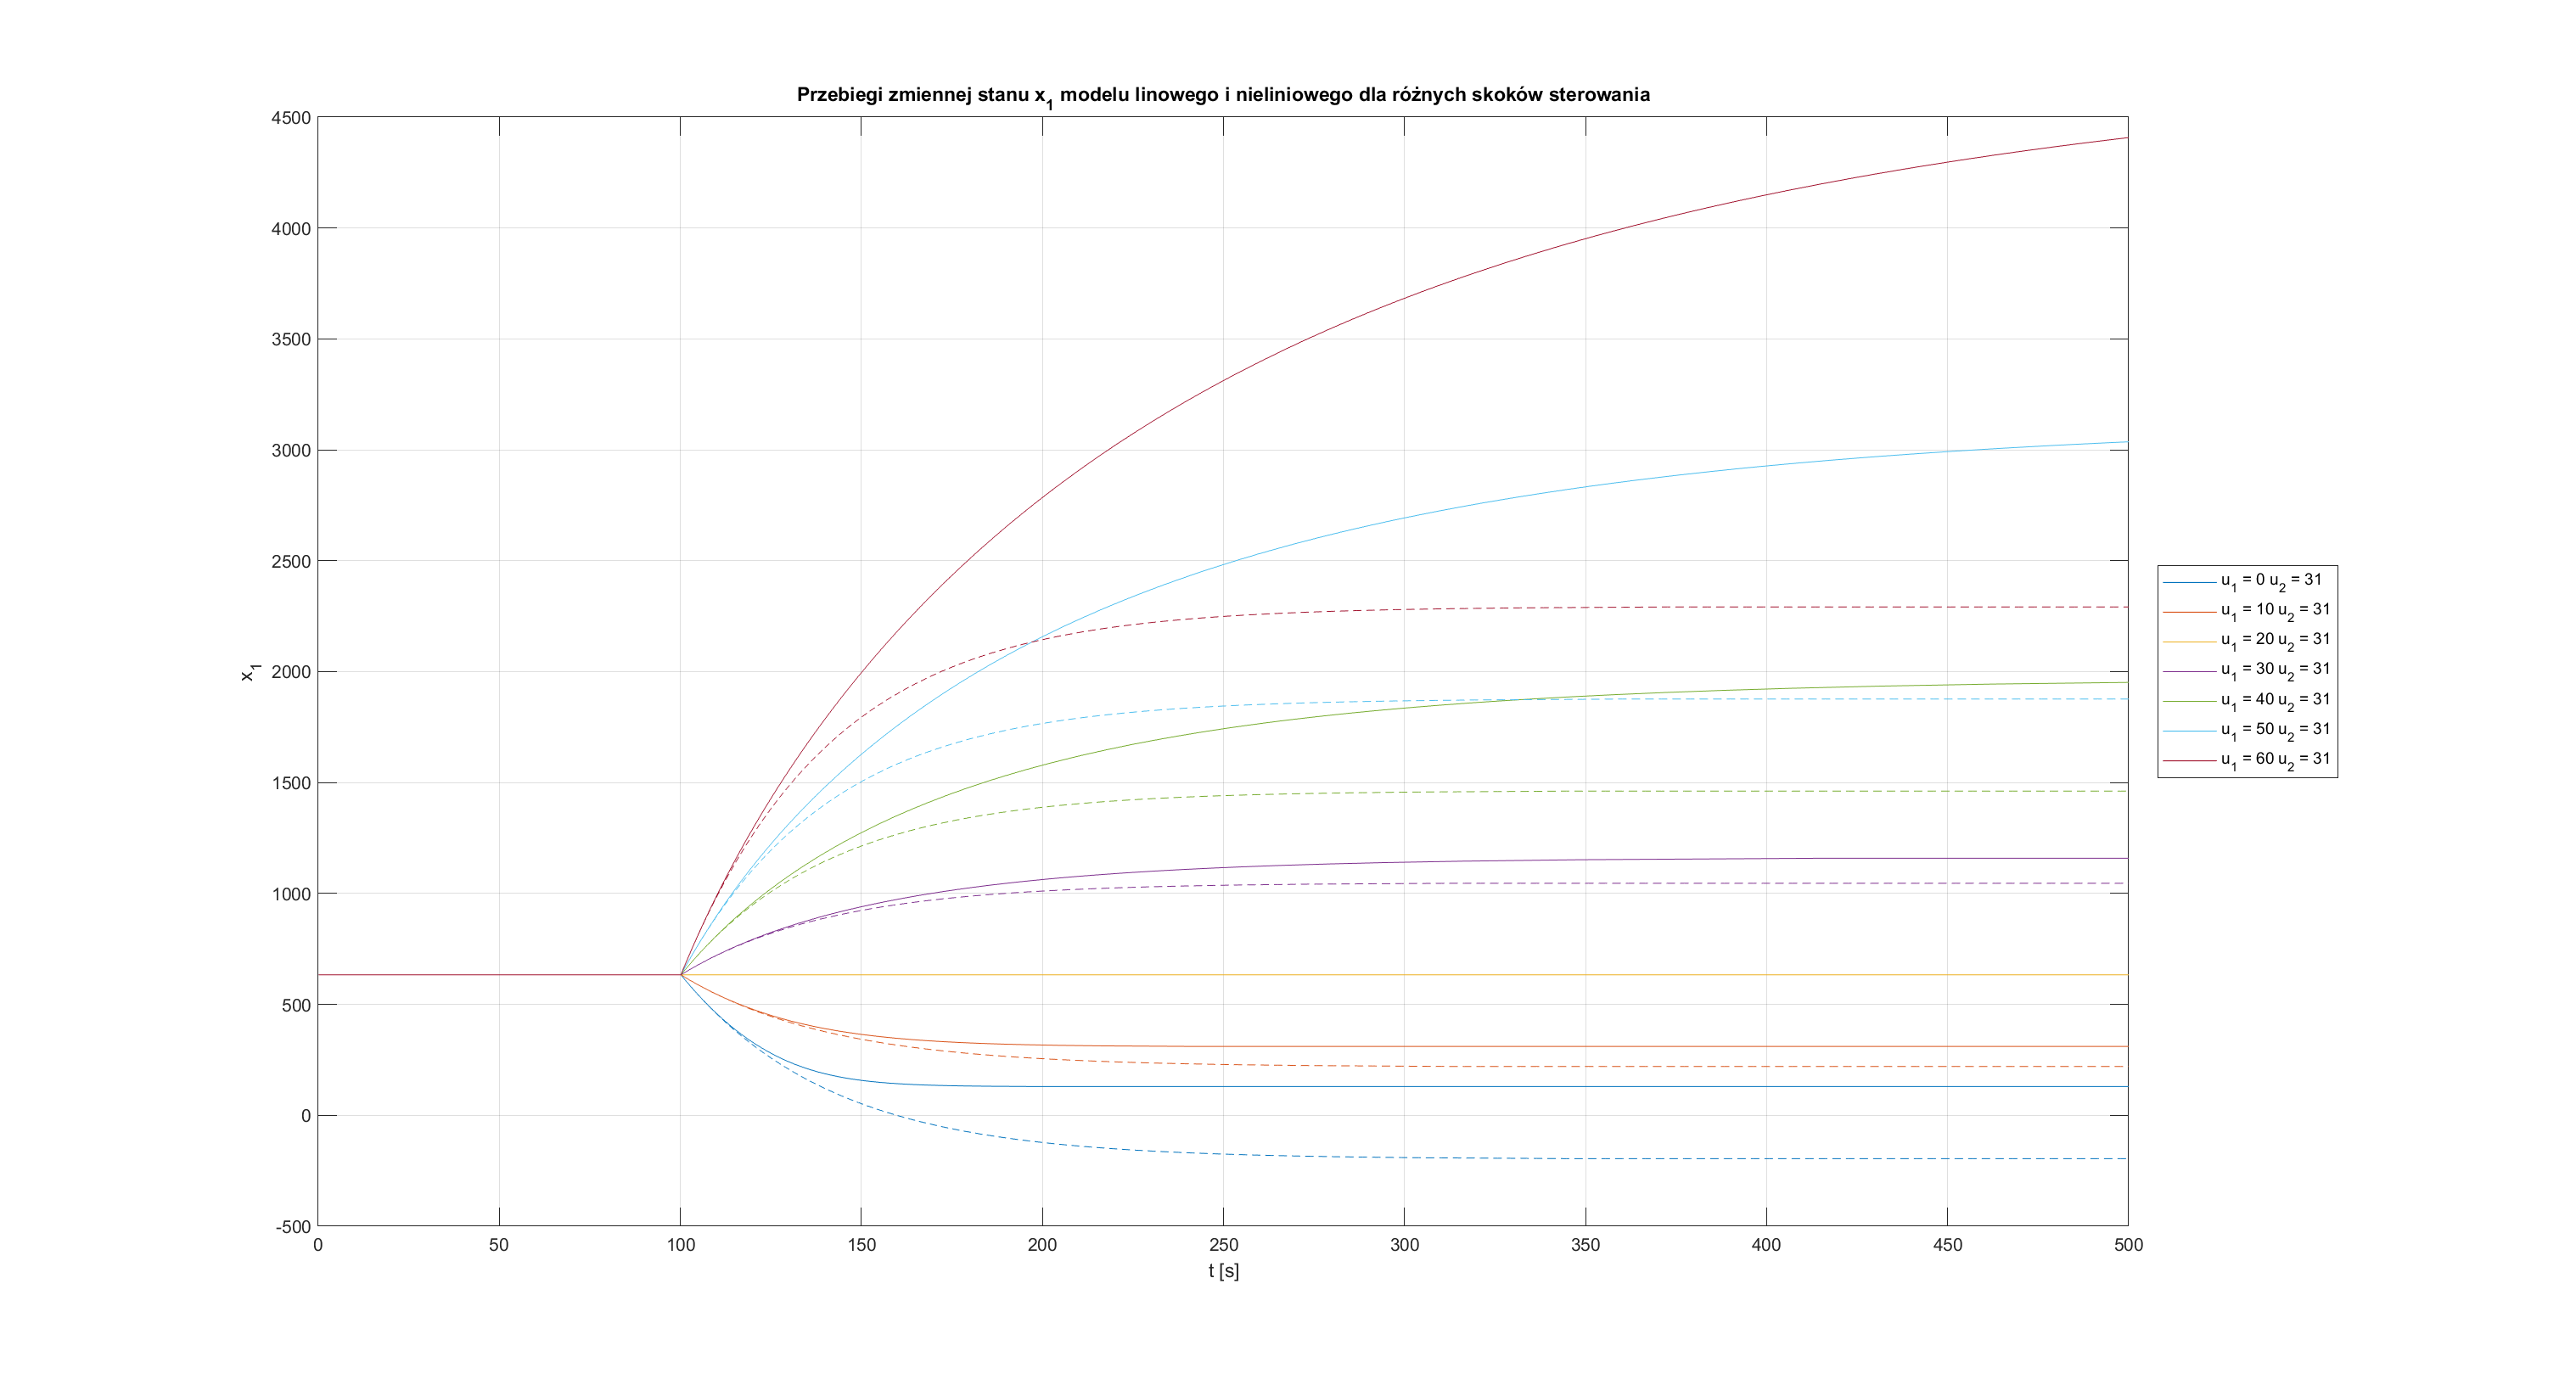
\includegraphics[scale=0.35]{images/x1_u1=60_u2=31_dt=0.1.eps}
    \caption{Porównanie modeli liniowych i nieliniowych}
\end{figure}

\begin{figure}[H]
    \centering
    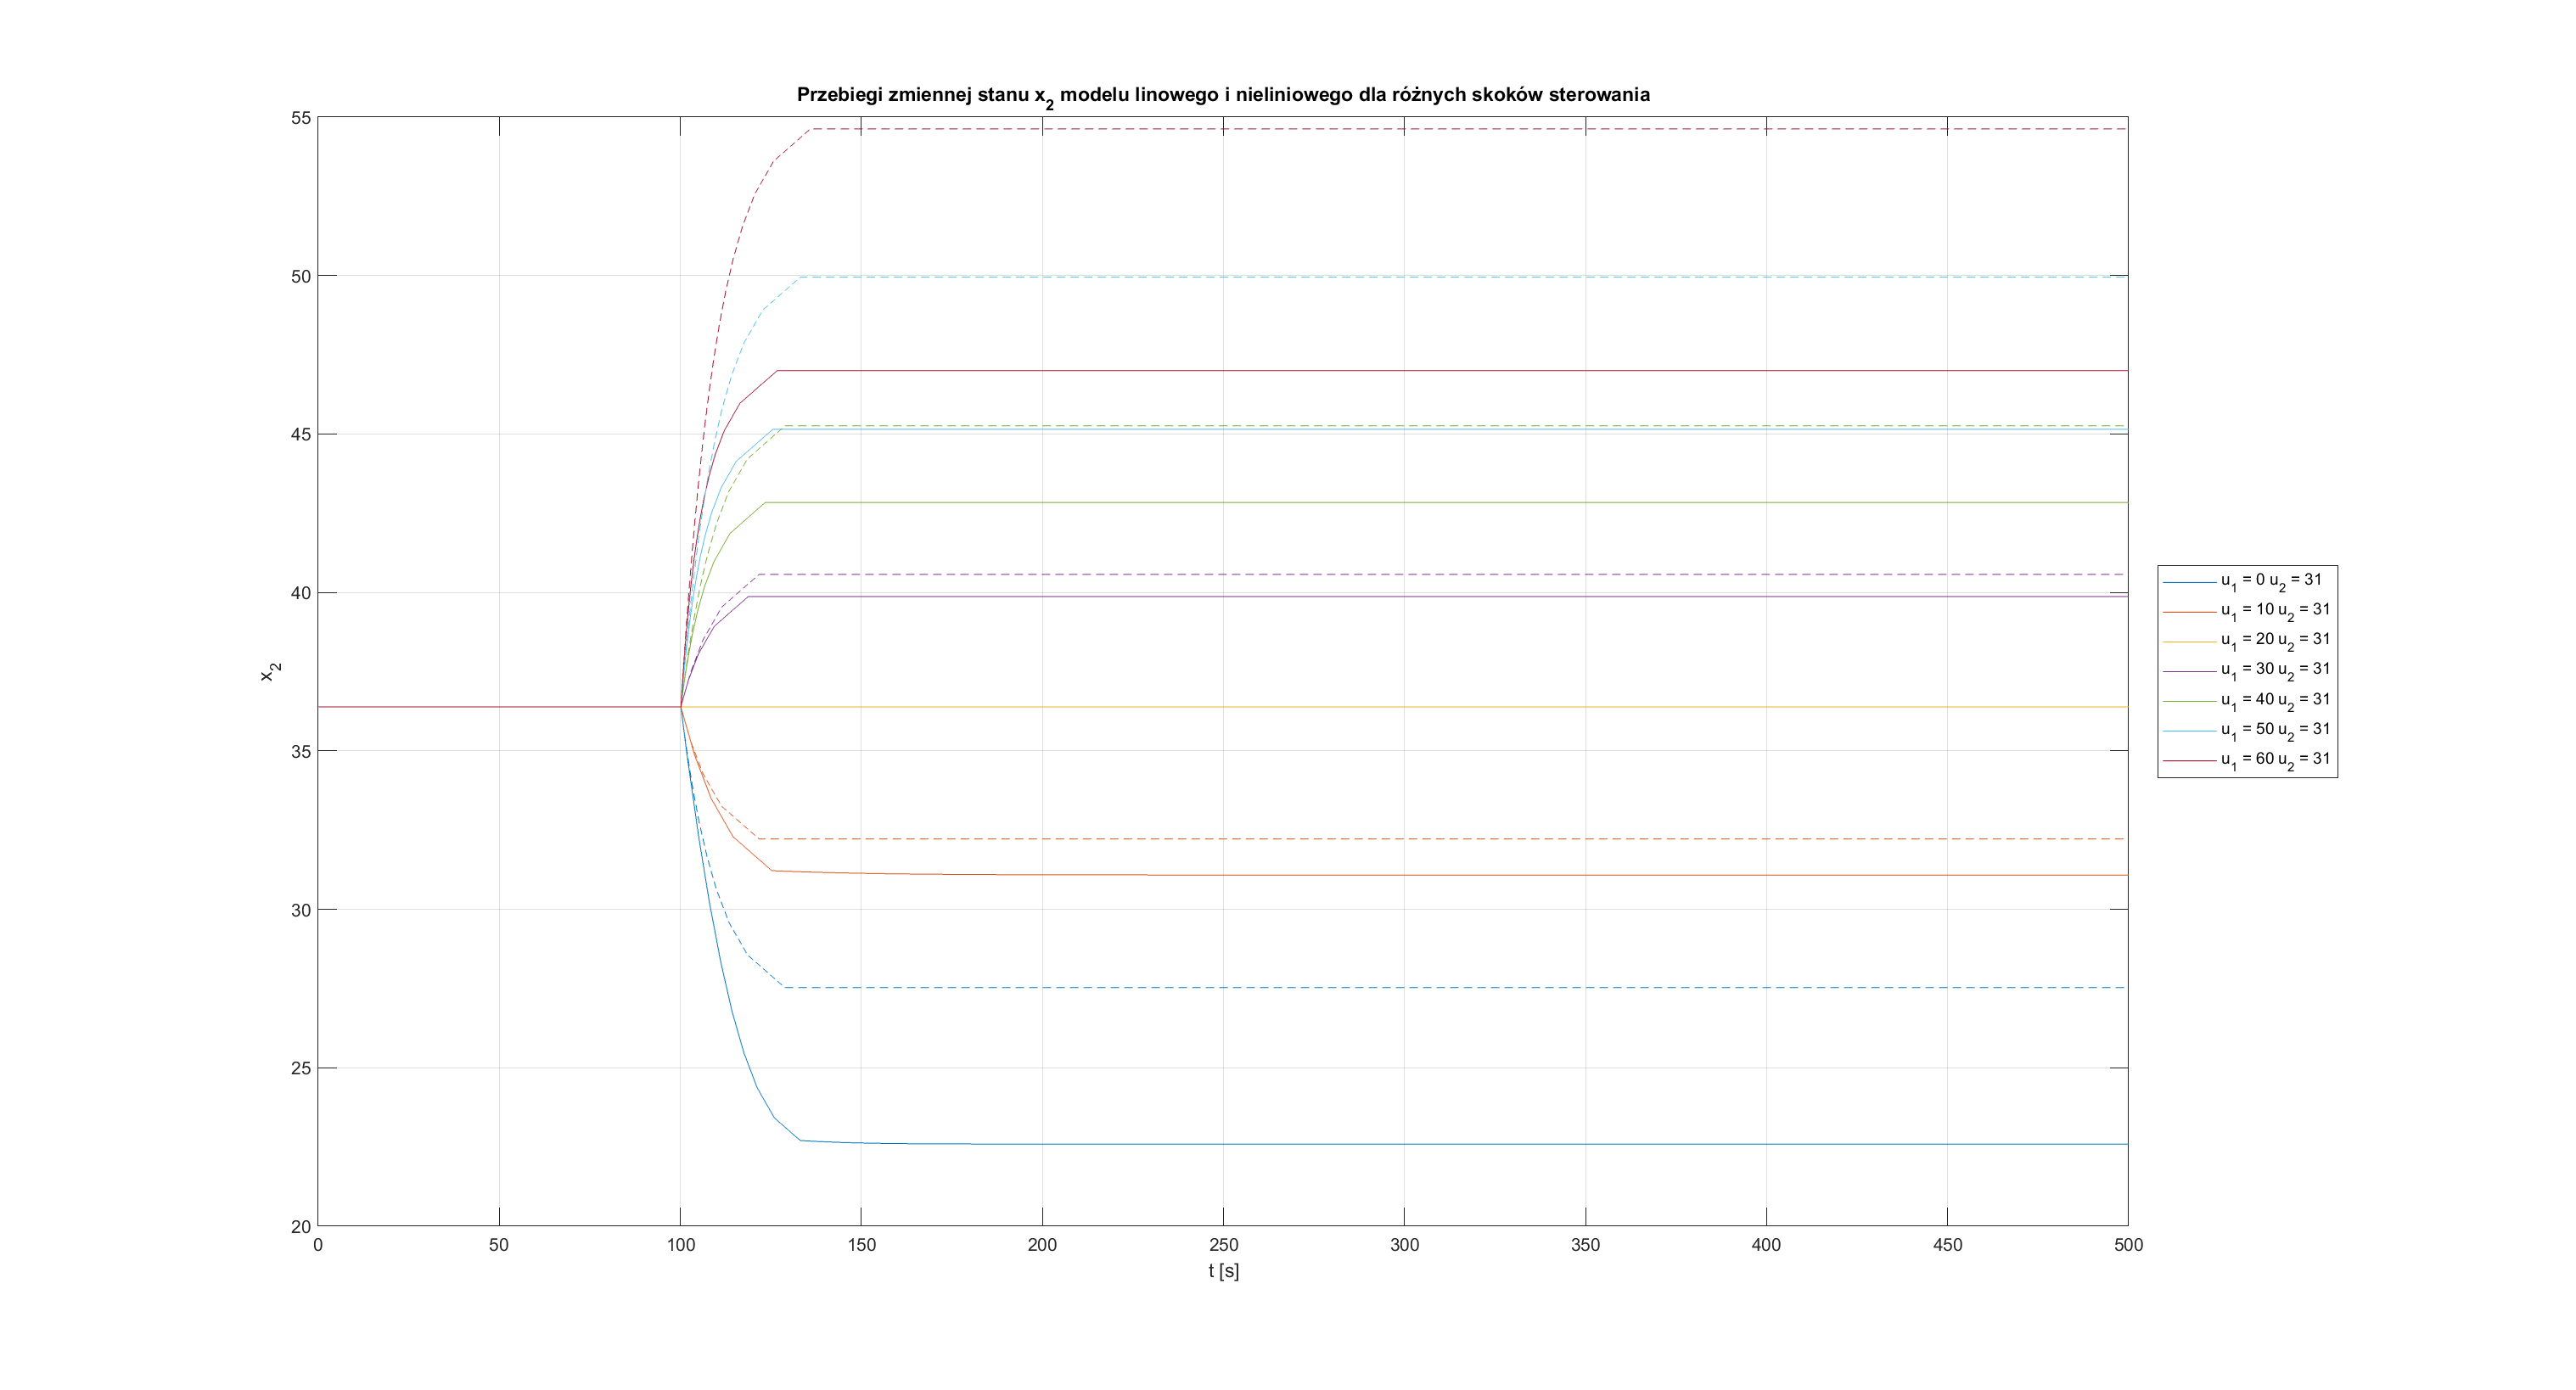
\includegraphics[scale=0.35]{images/x2_u1=60_u2=31_dt=0.1.eps}
    \caption{Porównanie modeli liniowych i nieliniowych}
\end{figure}

\begin{figure}[H]
    \centering
    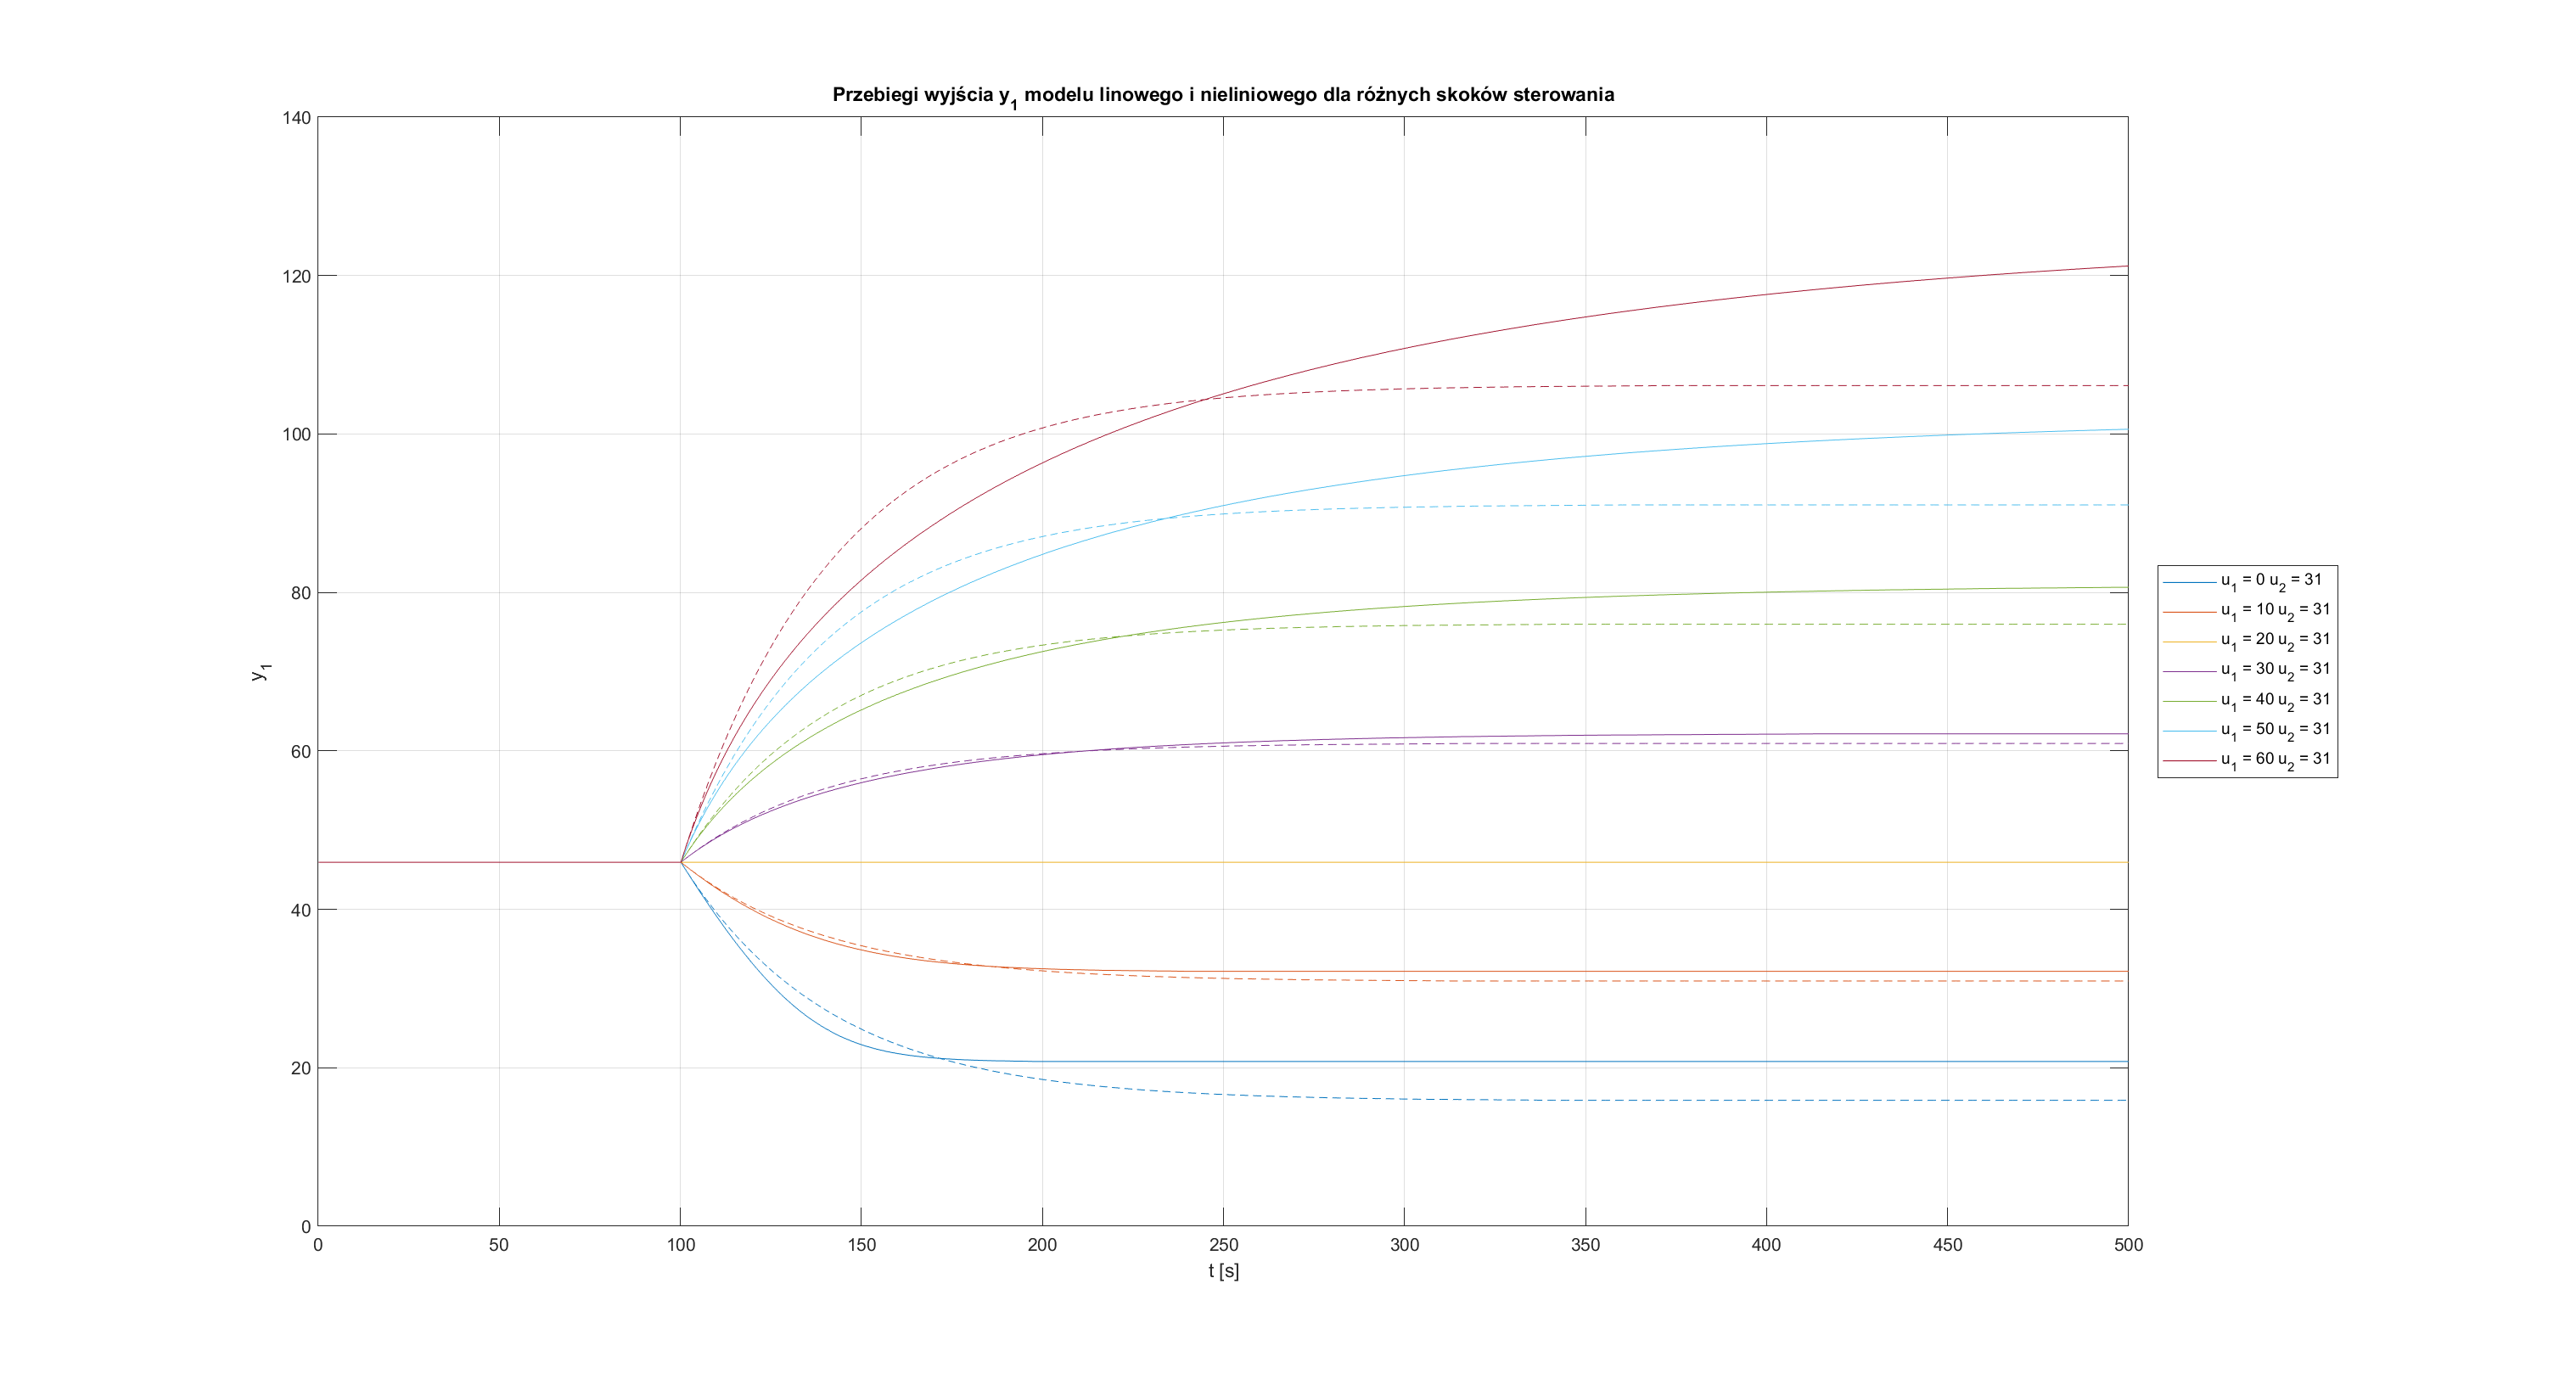
\includegraphics[scale=0.35]{images/y1_u1=60_u2=31_dt=0.1.eps}
    \caption{Porównanie modeli liniowych i nieliniowych}
\end{figure}

\begin{figure}[H]
    \centering
    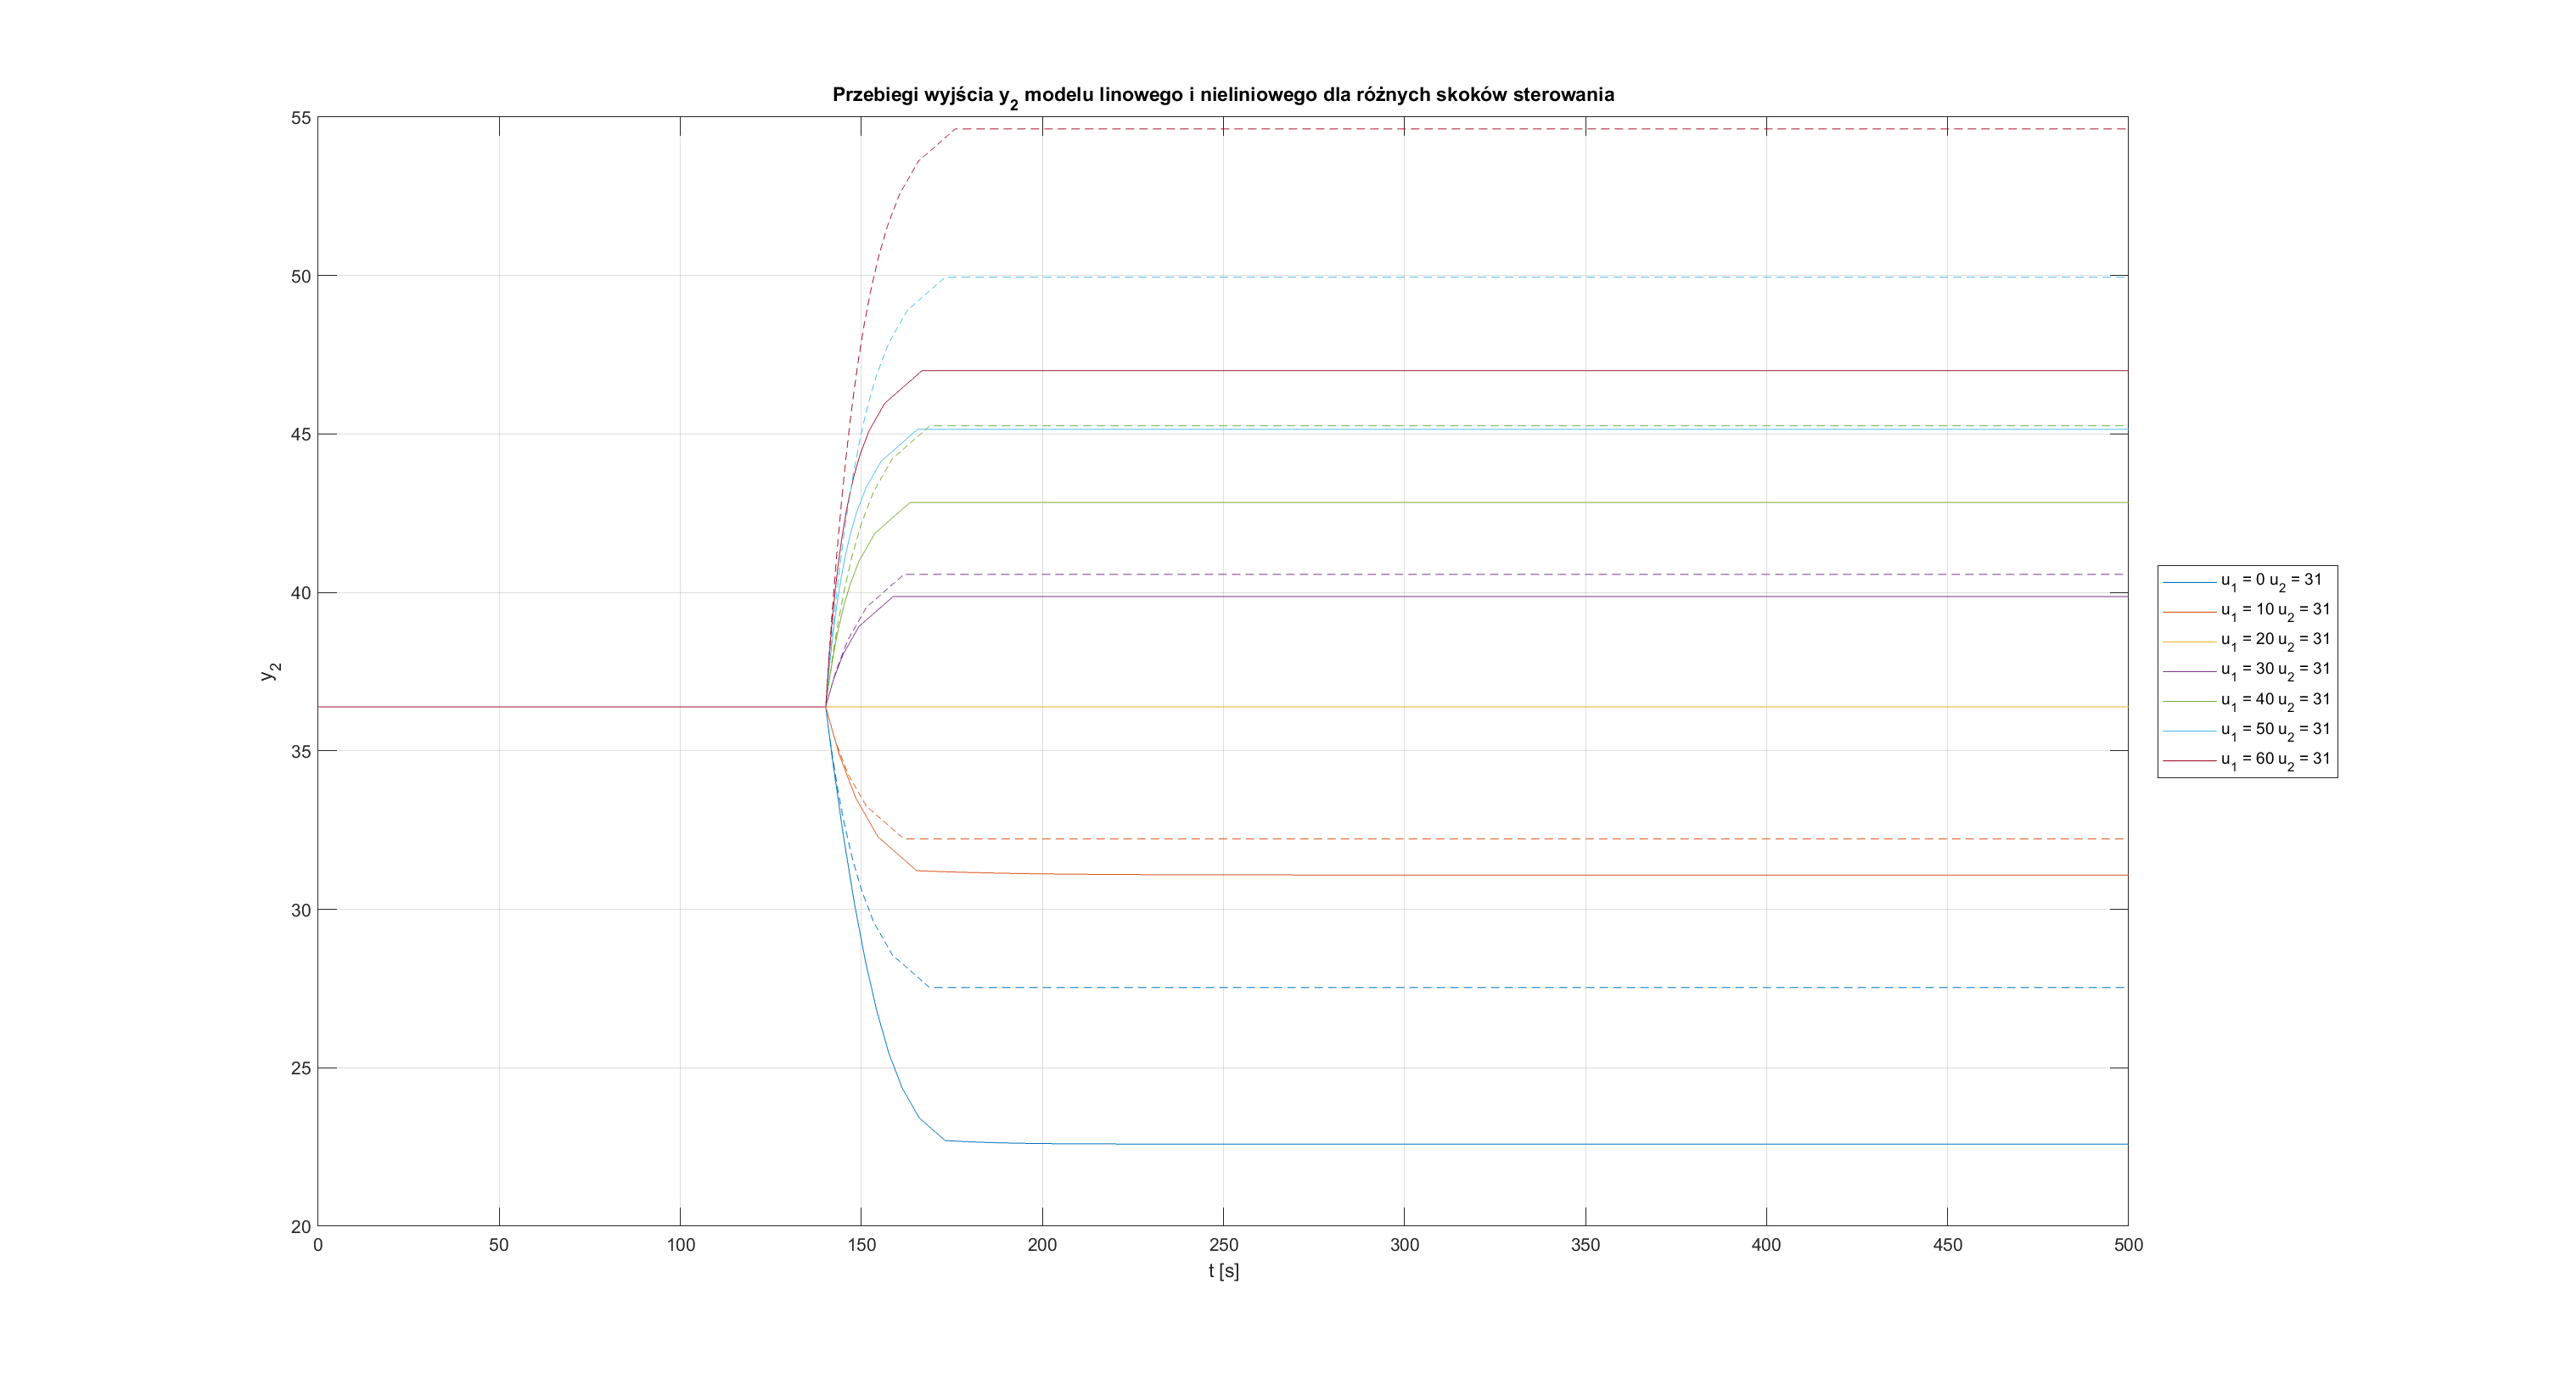
\includegraphics[scale=0.35]{images/y2_u1=60_u2=31_dt=0.1.eps}
    \caption{Porównanie modeli liniowych i nieliniowych}
\end{figure}

W kolejnym sprawdzano zachowanie układu dla różnych wartości $u_2$, resztę pozostawiając bez zmian.

\begin{figure}[H]
    \centering
    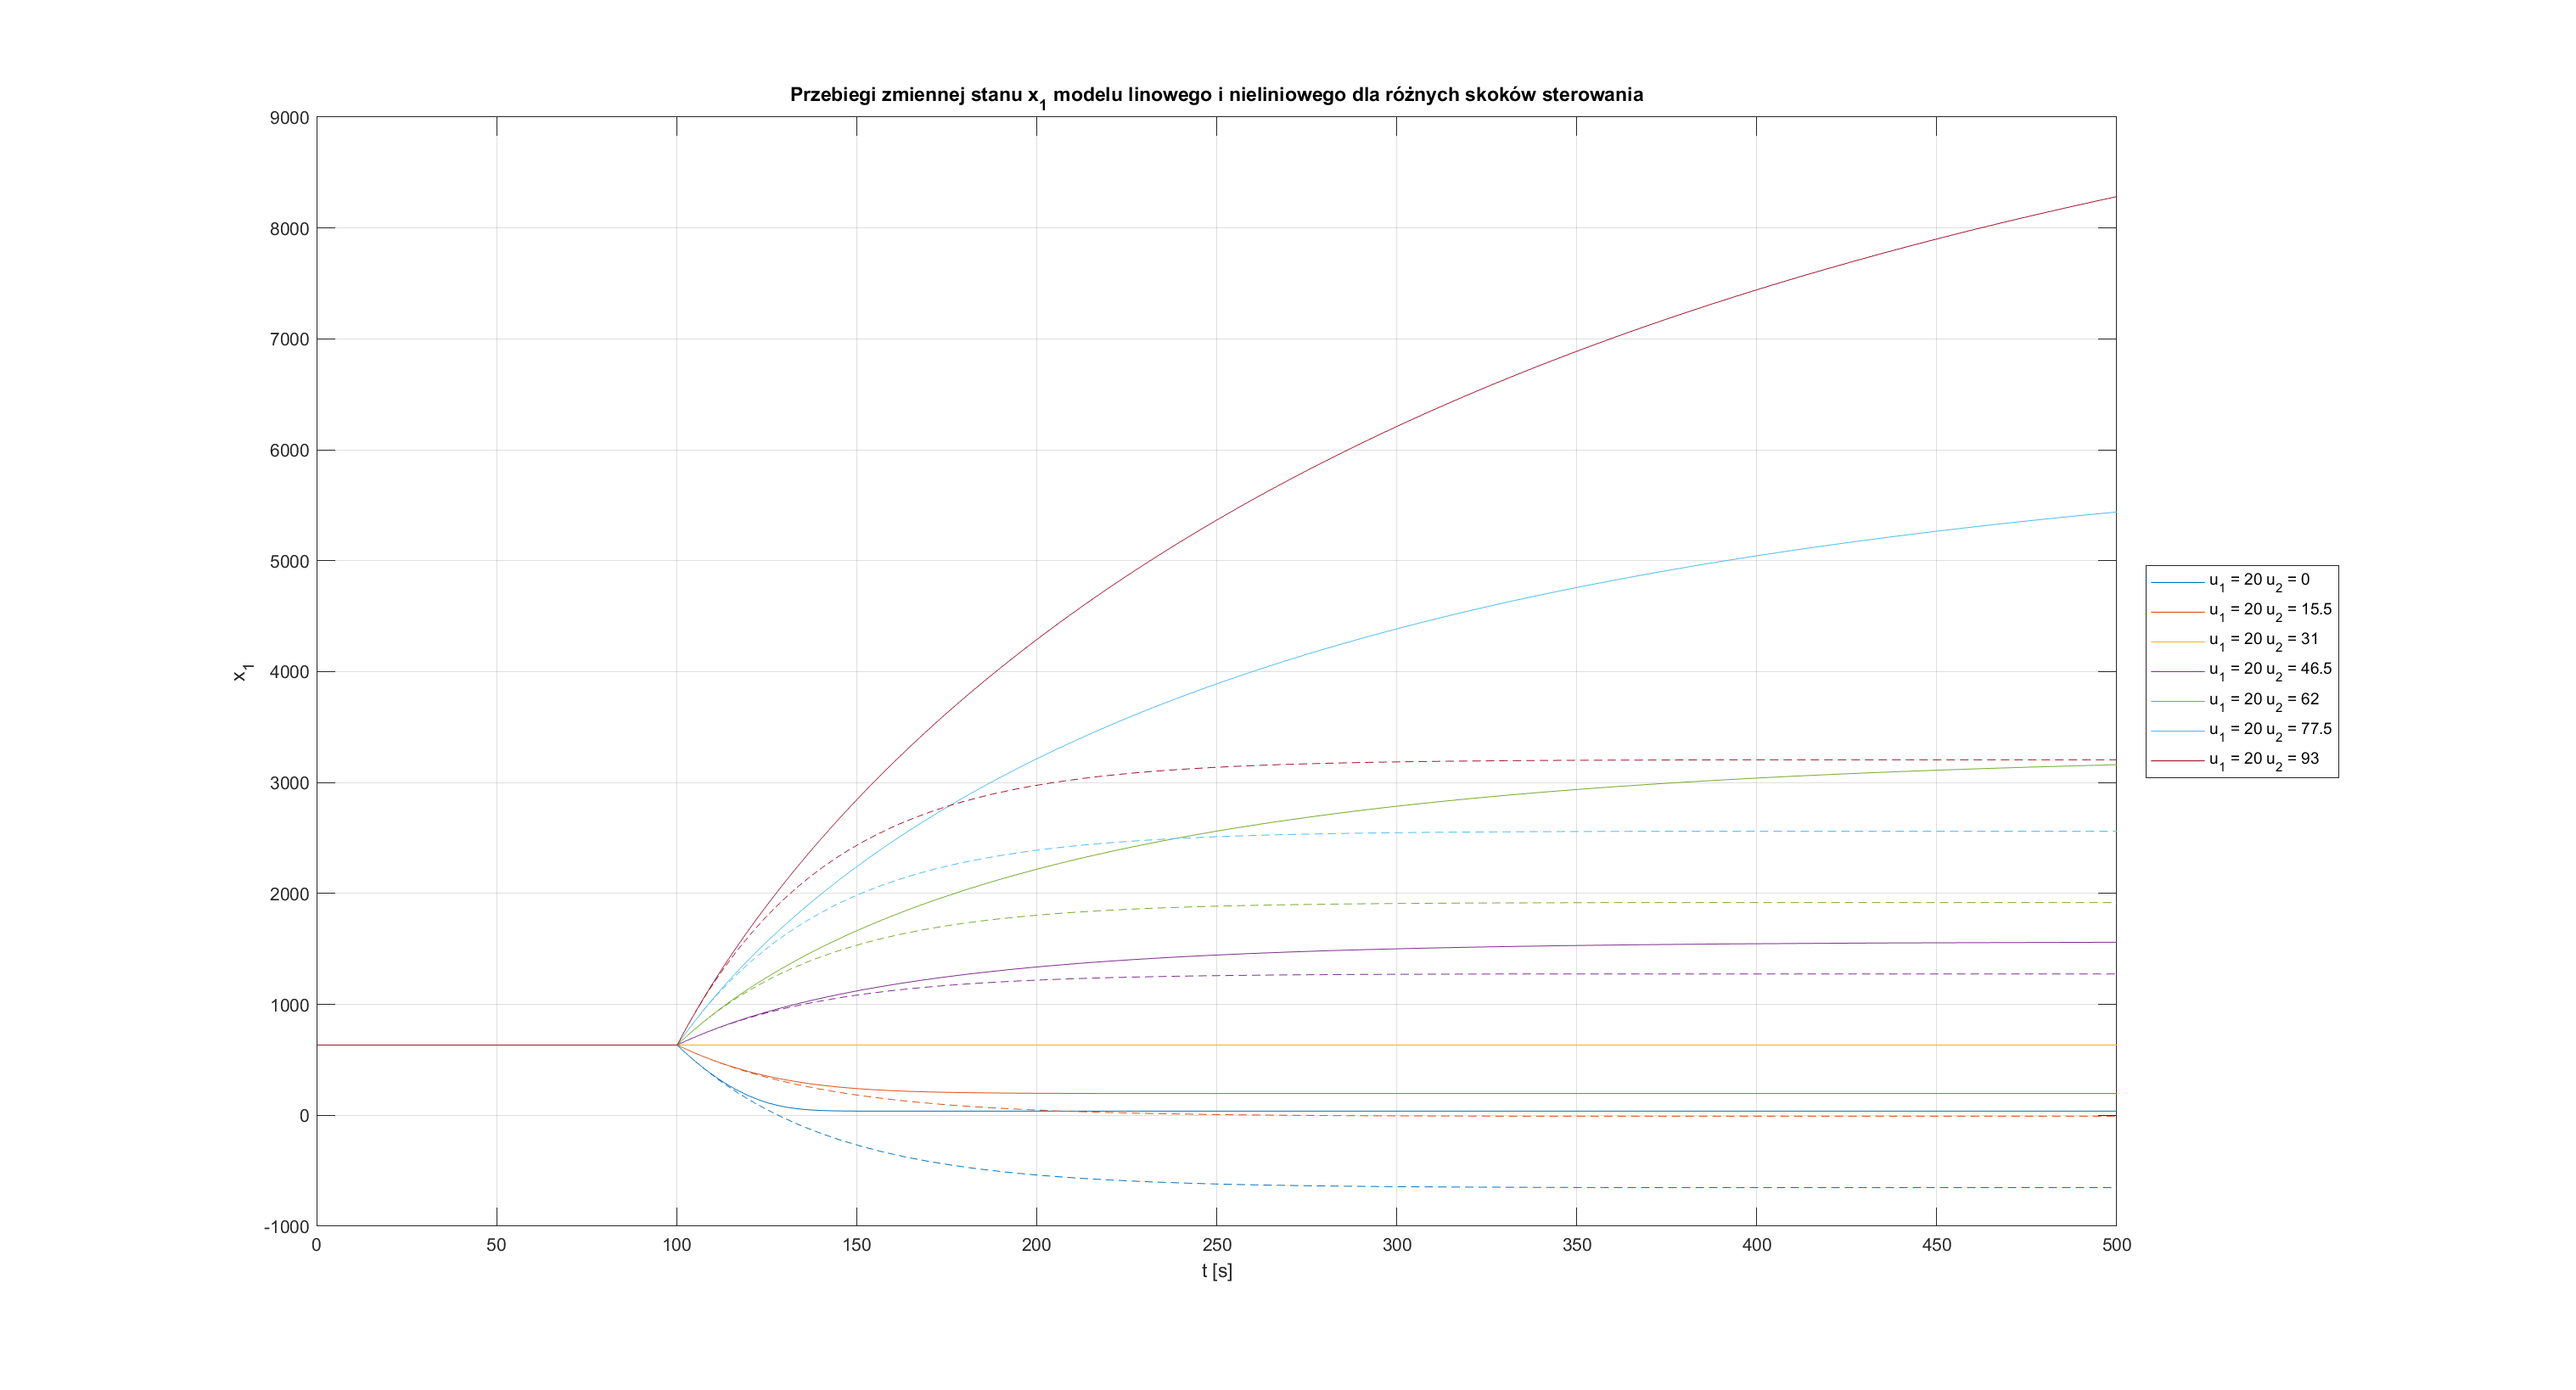
\includegraphics[scale=0.35]{images/x1_u1=20_u2=93_dt=0.1.eps}
    \caption{Porównanie modeli liniowych i nieliniowych}
\end{figure}

\begin{figure}[H]
    \centering
    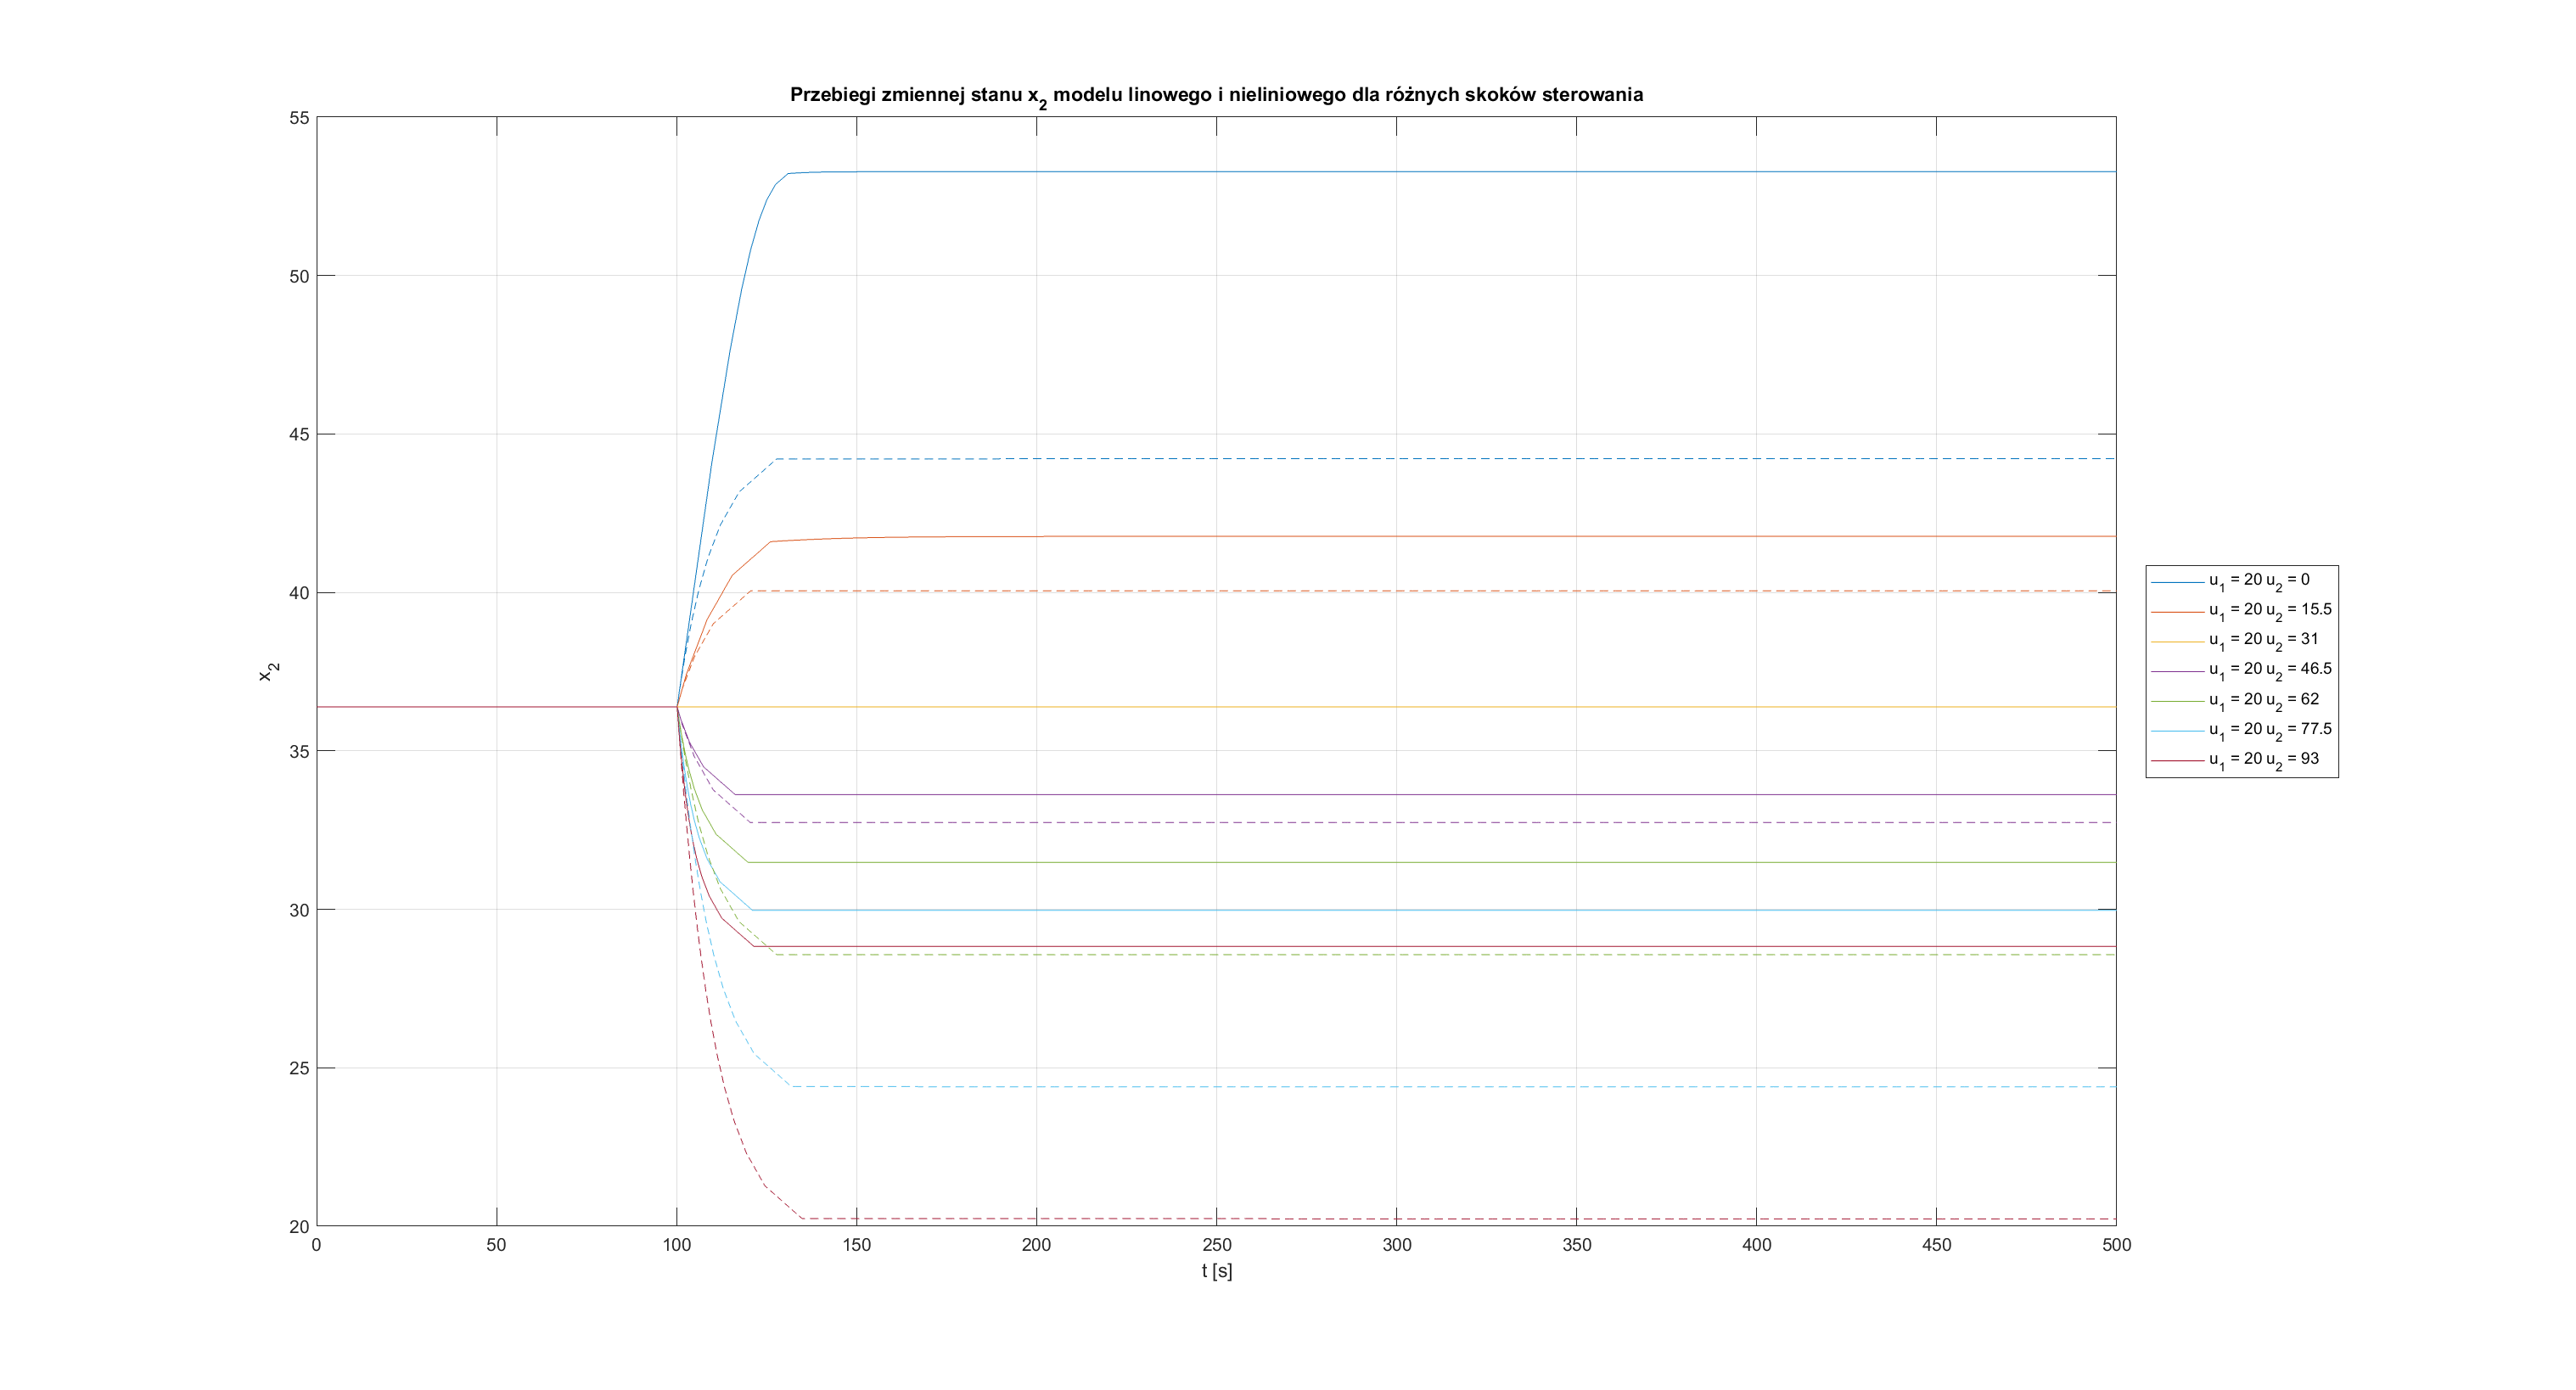
\includegraphics[scale=0.35]{images/x2_u1=20_u2=93_dt=0.1.eps}
    \caption{Porównanie modeli liniowych i nieliniowych}
\end{figure}

\begin{figure}[H]
    \centering
    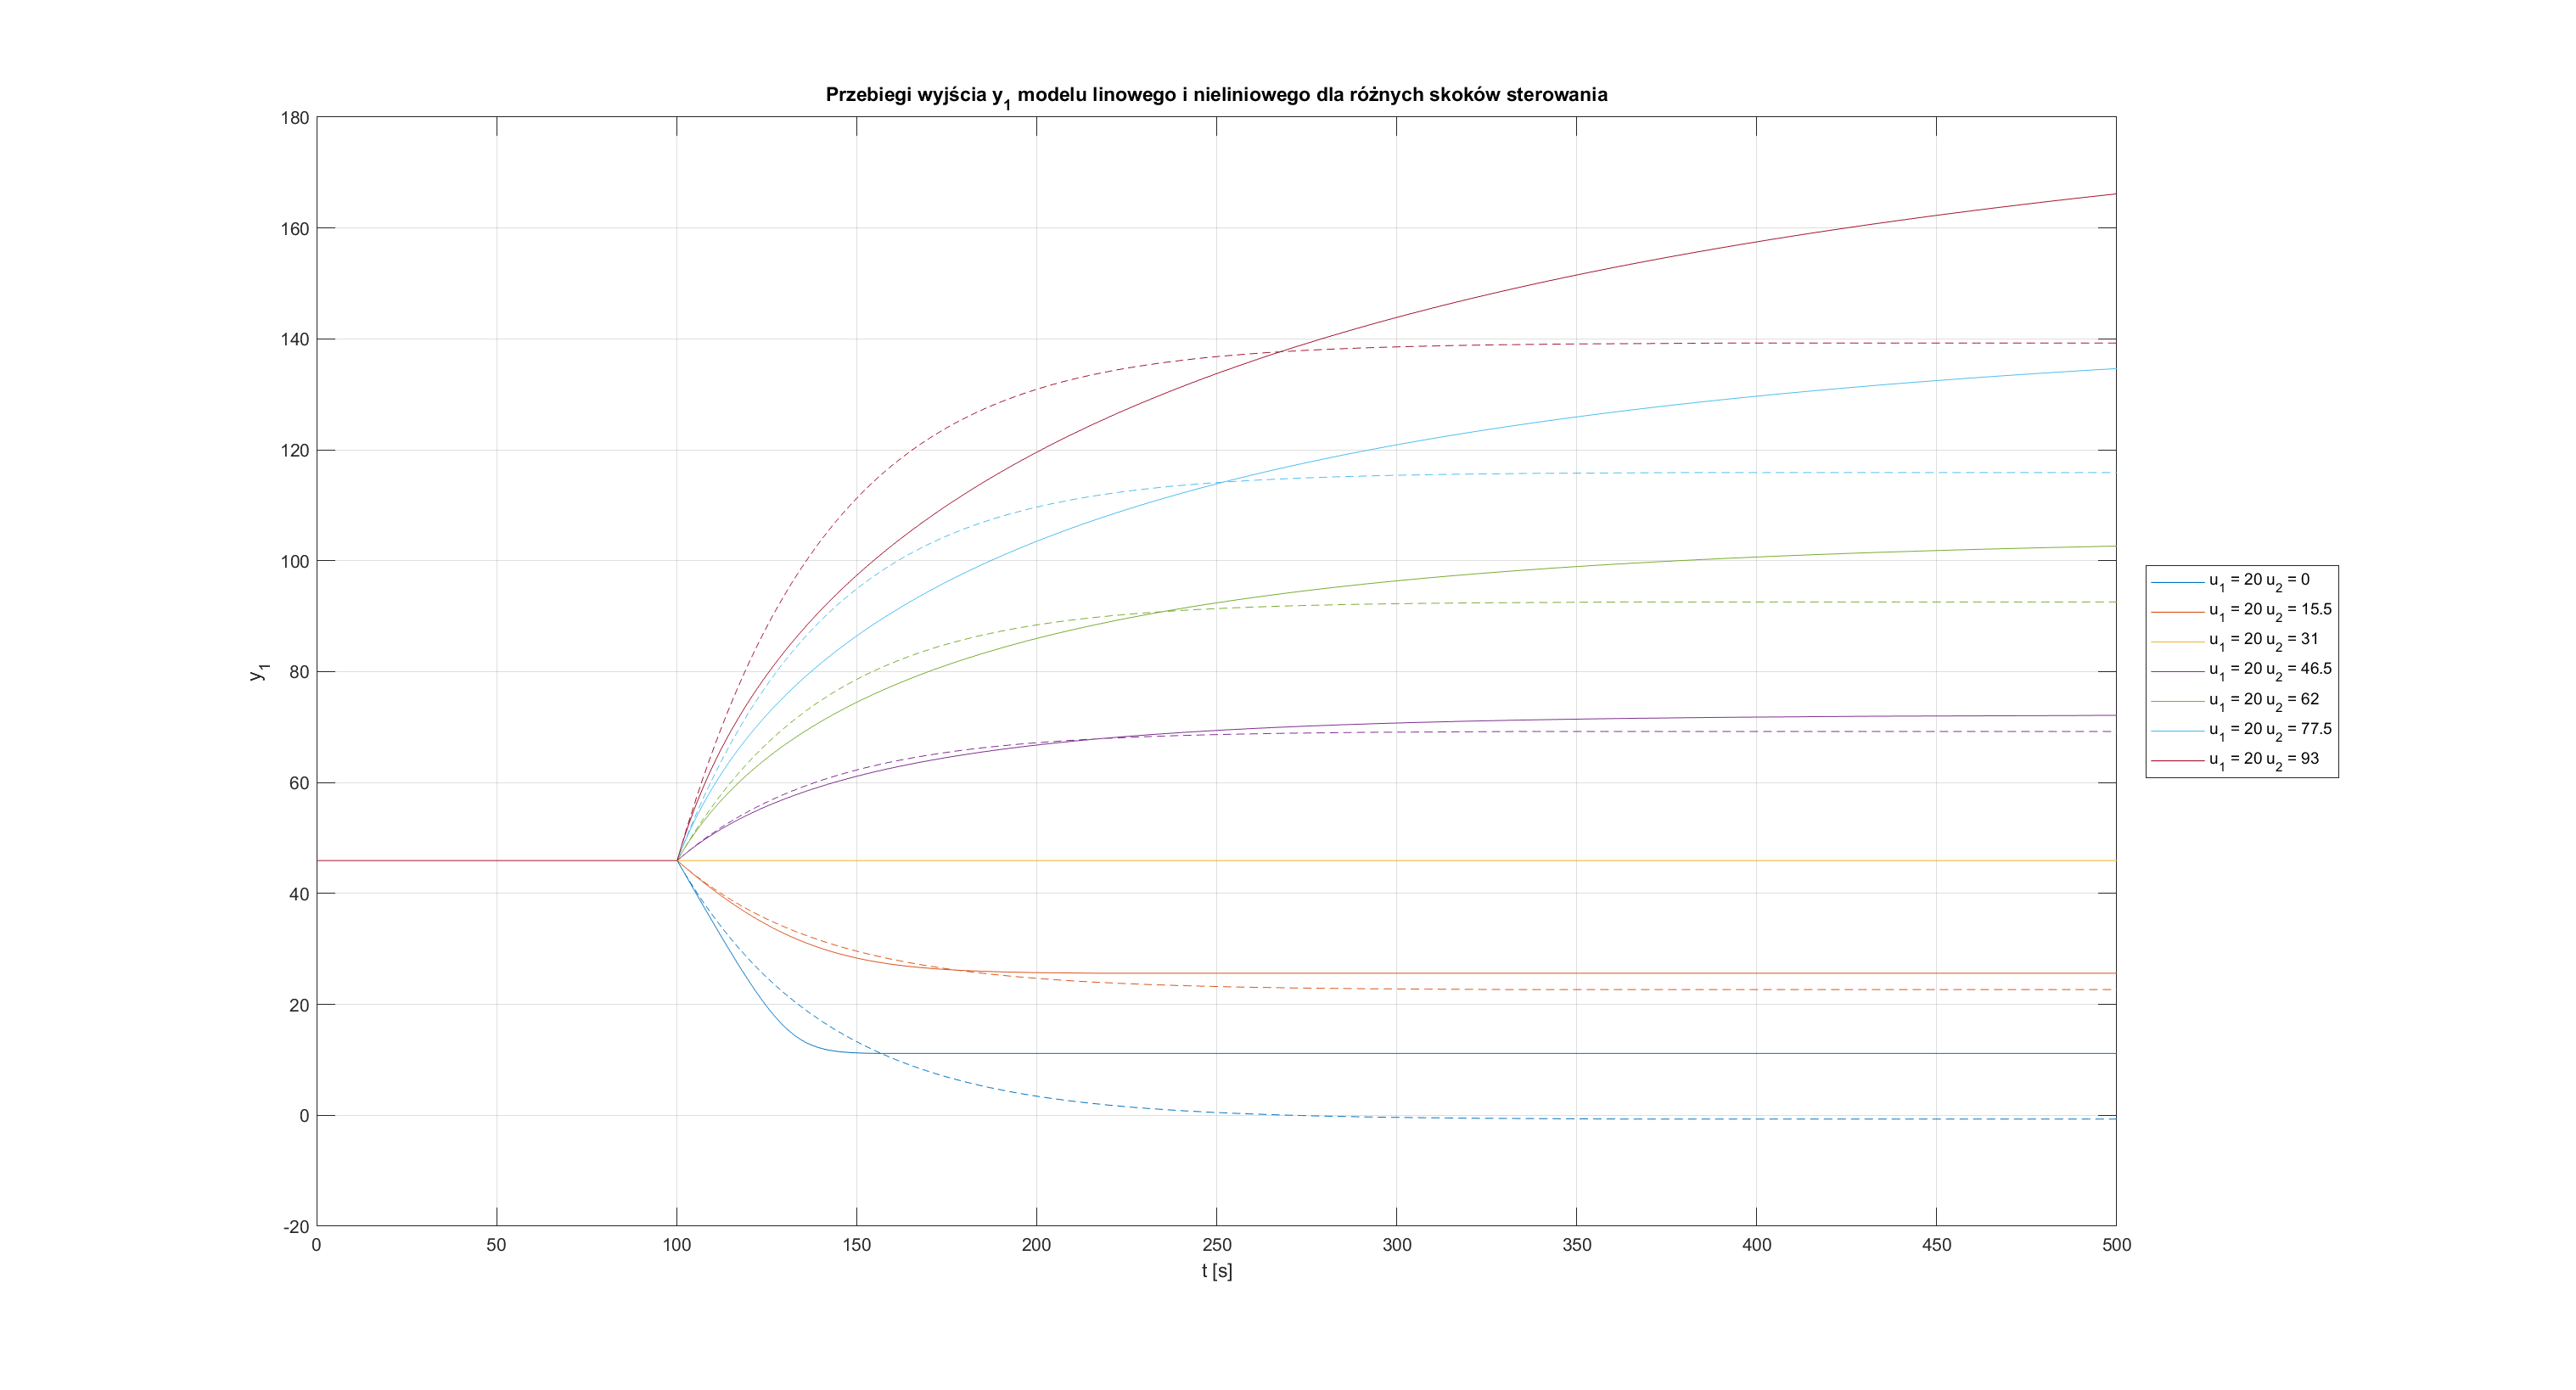
\includegraphics[scale=0.35]{images/y1_u1=20_u2=93_dt=0.1.eps}
    \caption{Porównanie modeli liniowych i nieliniowych}
\end{figure}

\begin{figure}[H]
    \centering
    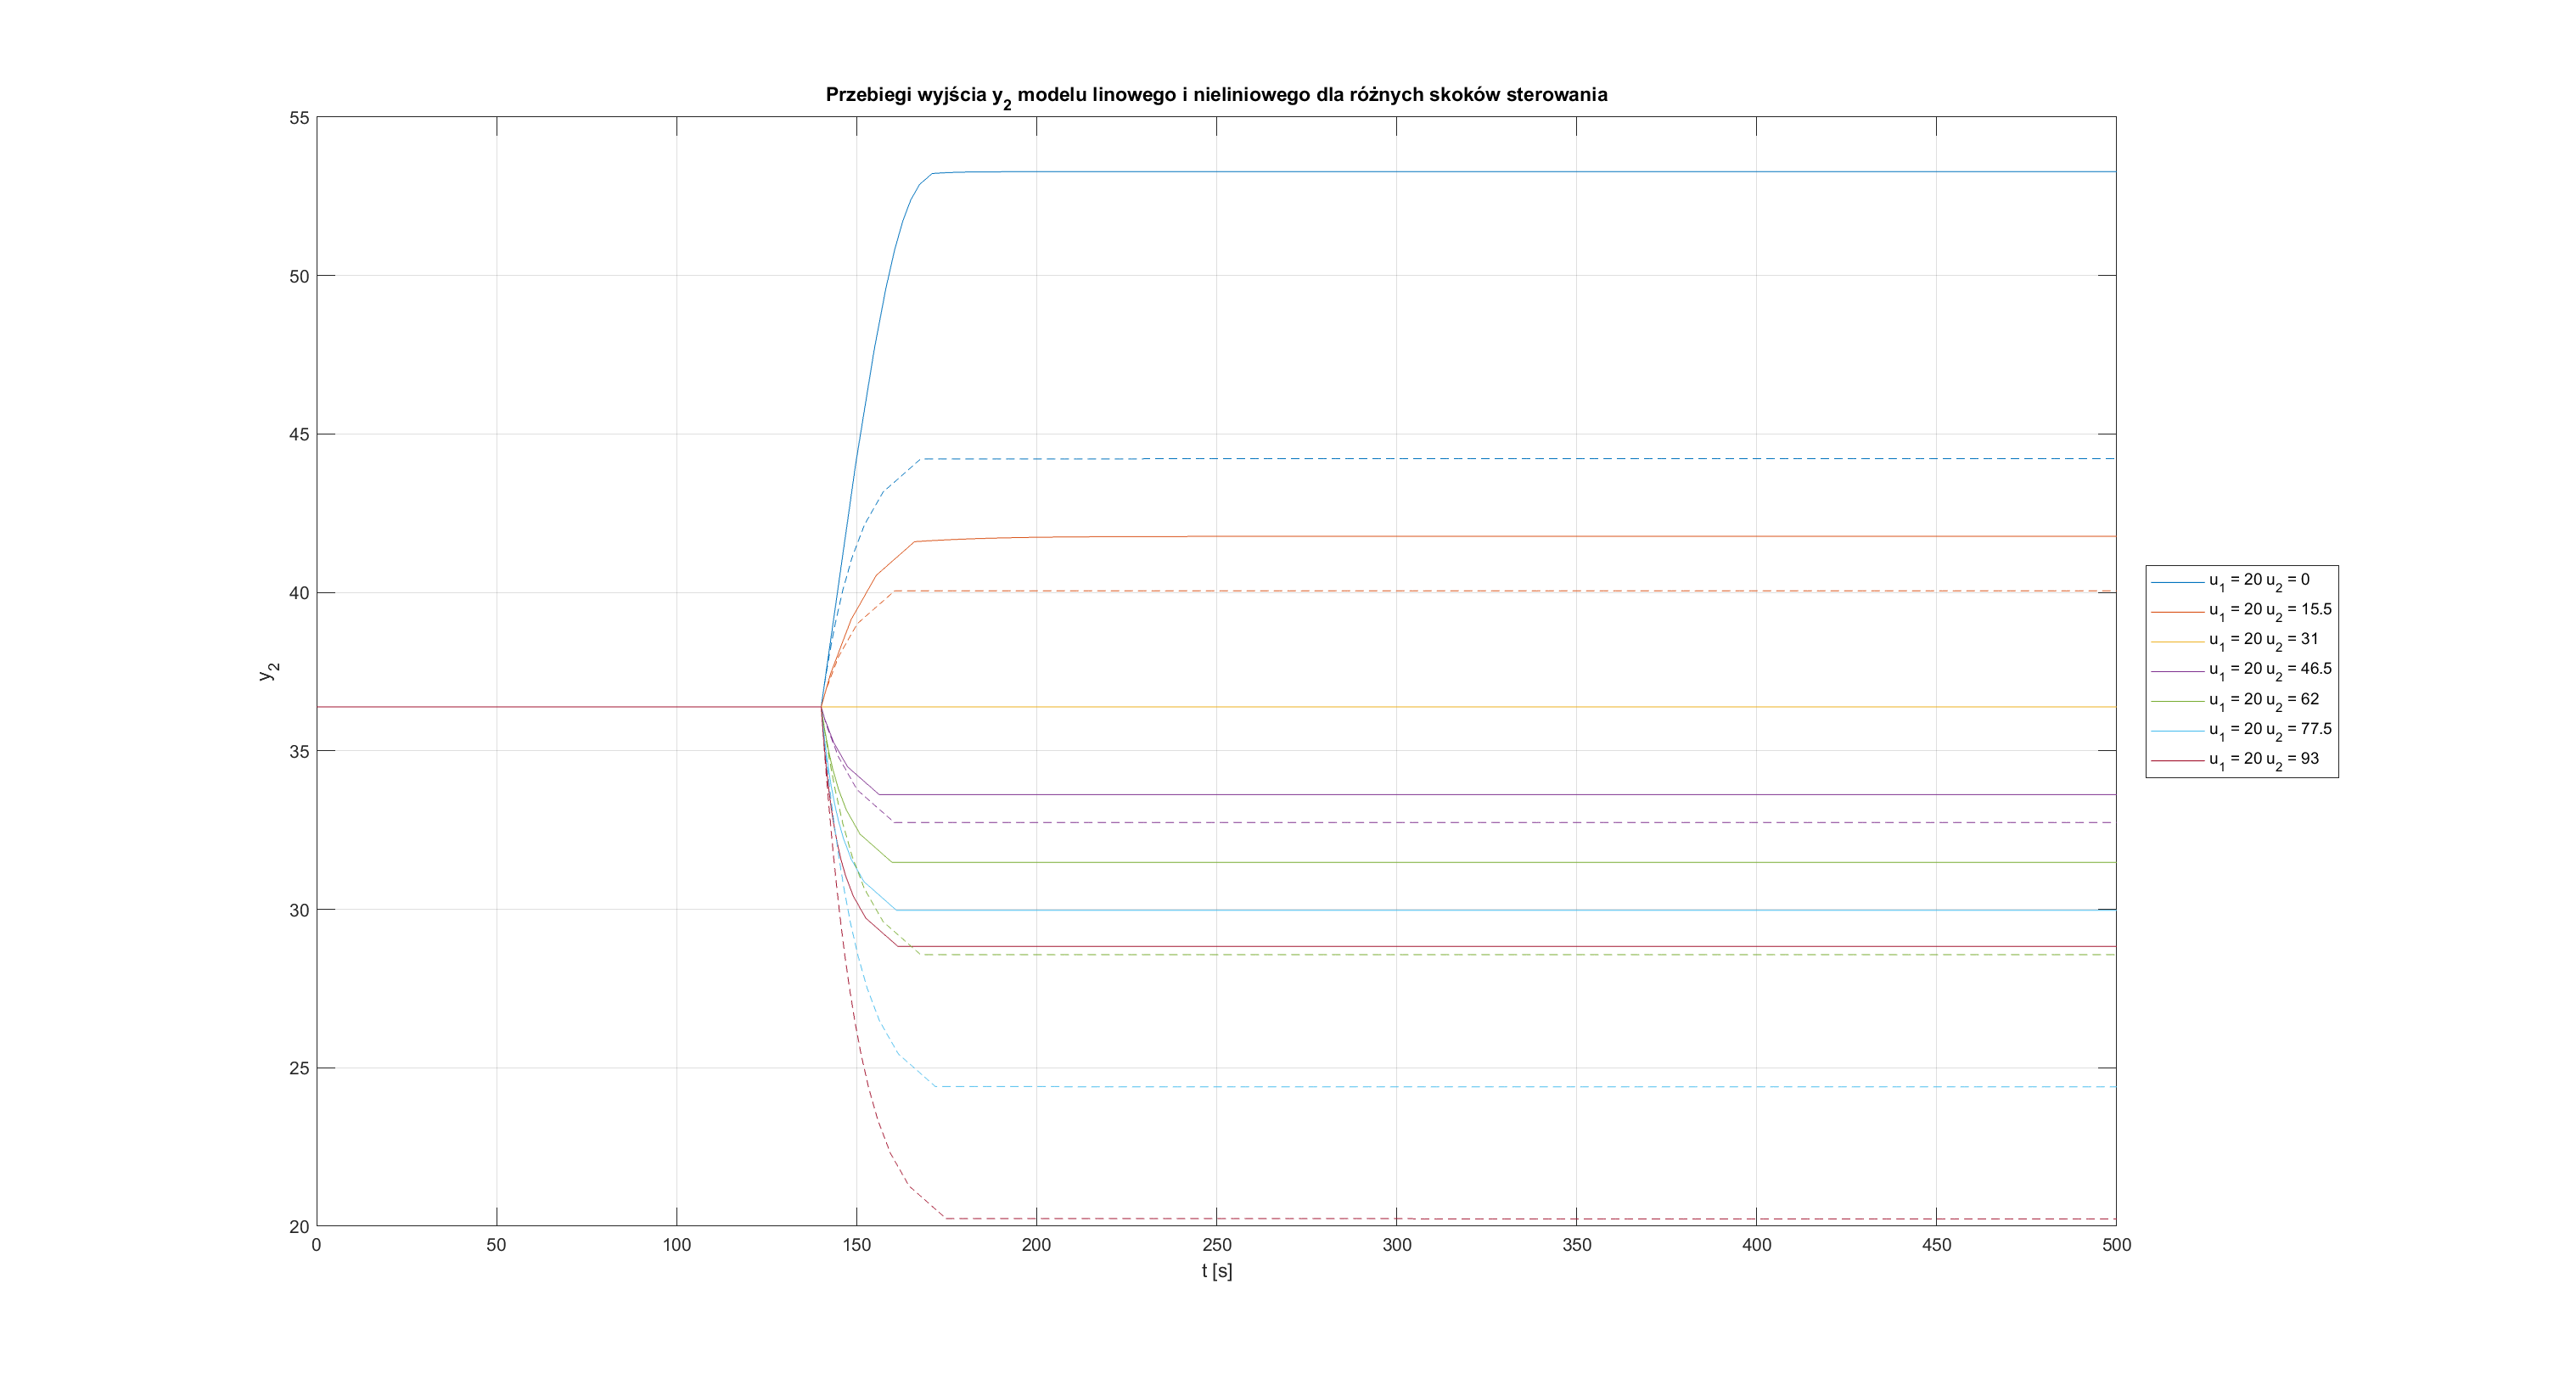
\includegraphics[scale=0.35]{images/y2_u1=20_u2=93_dt=0.1.eps}
    \caption{Porównanie modeli liniowych i nieliniowych}
\end{figure}

Dalej sprawdzono zachowanie układu przy zmianach wejścia zakłócającego $v_1$.

\begin{figure}[H]
    \centering
    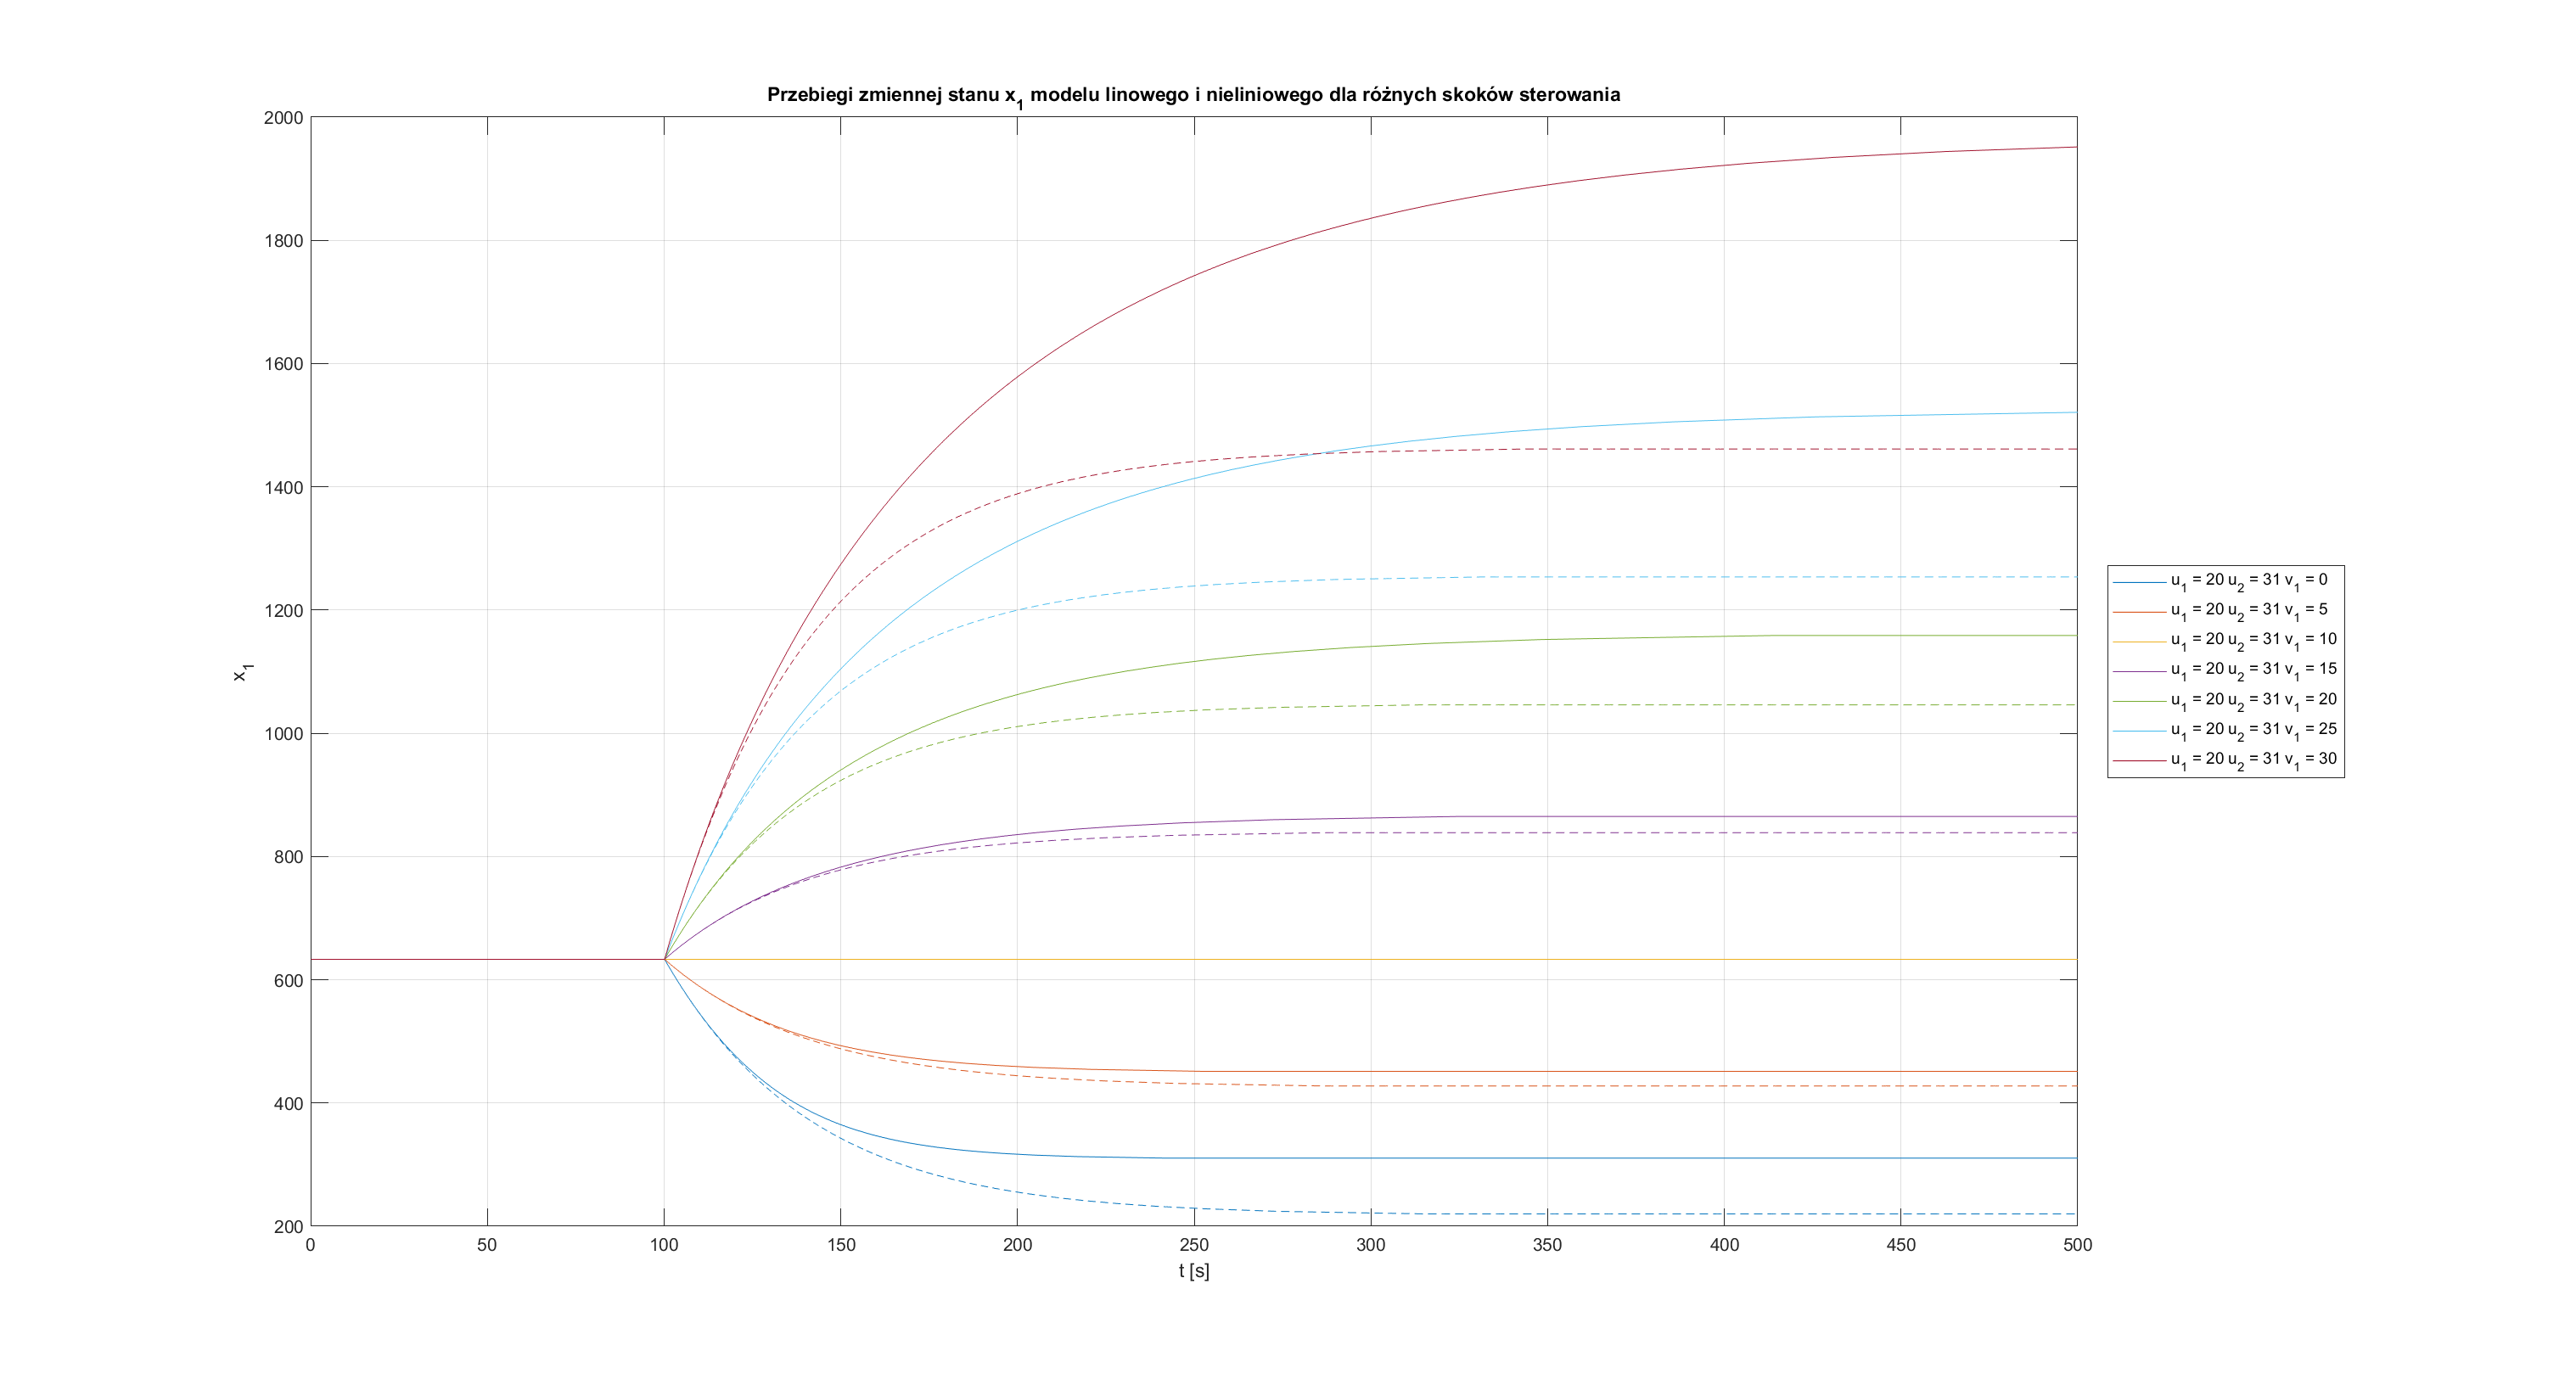
\includegraphics[scale=0.35]{images/x1_u1=20_u2=31_v1=30_dt=0.1.eps}
    \caption{Porównanie modeli liniowych i nieliniowych}
\end{figure}

\begin{figure}[H]
    \centering
    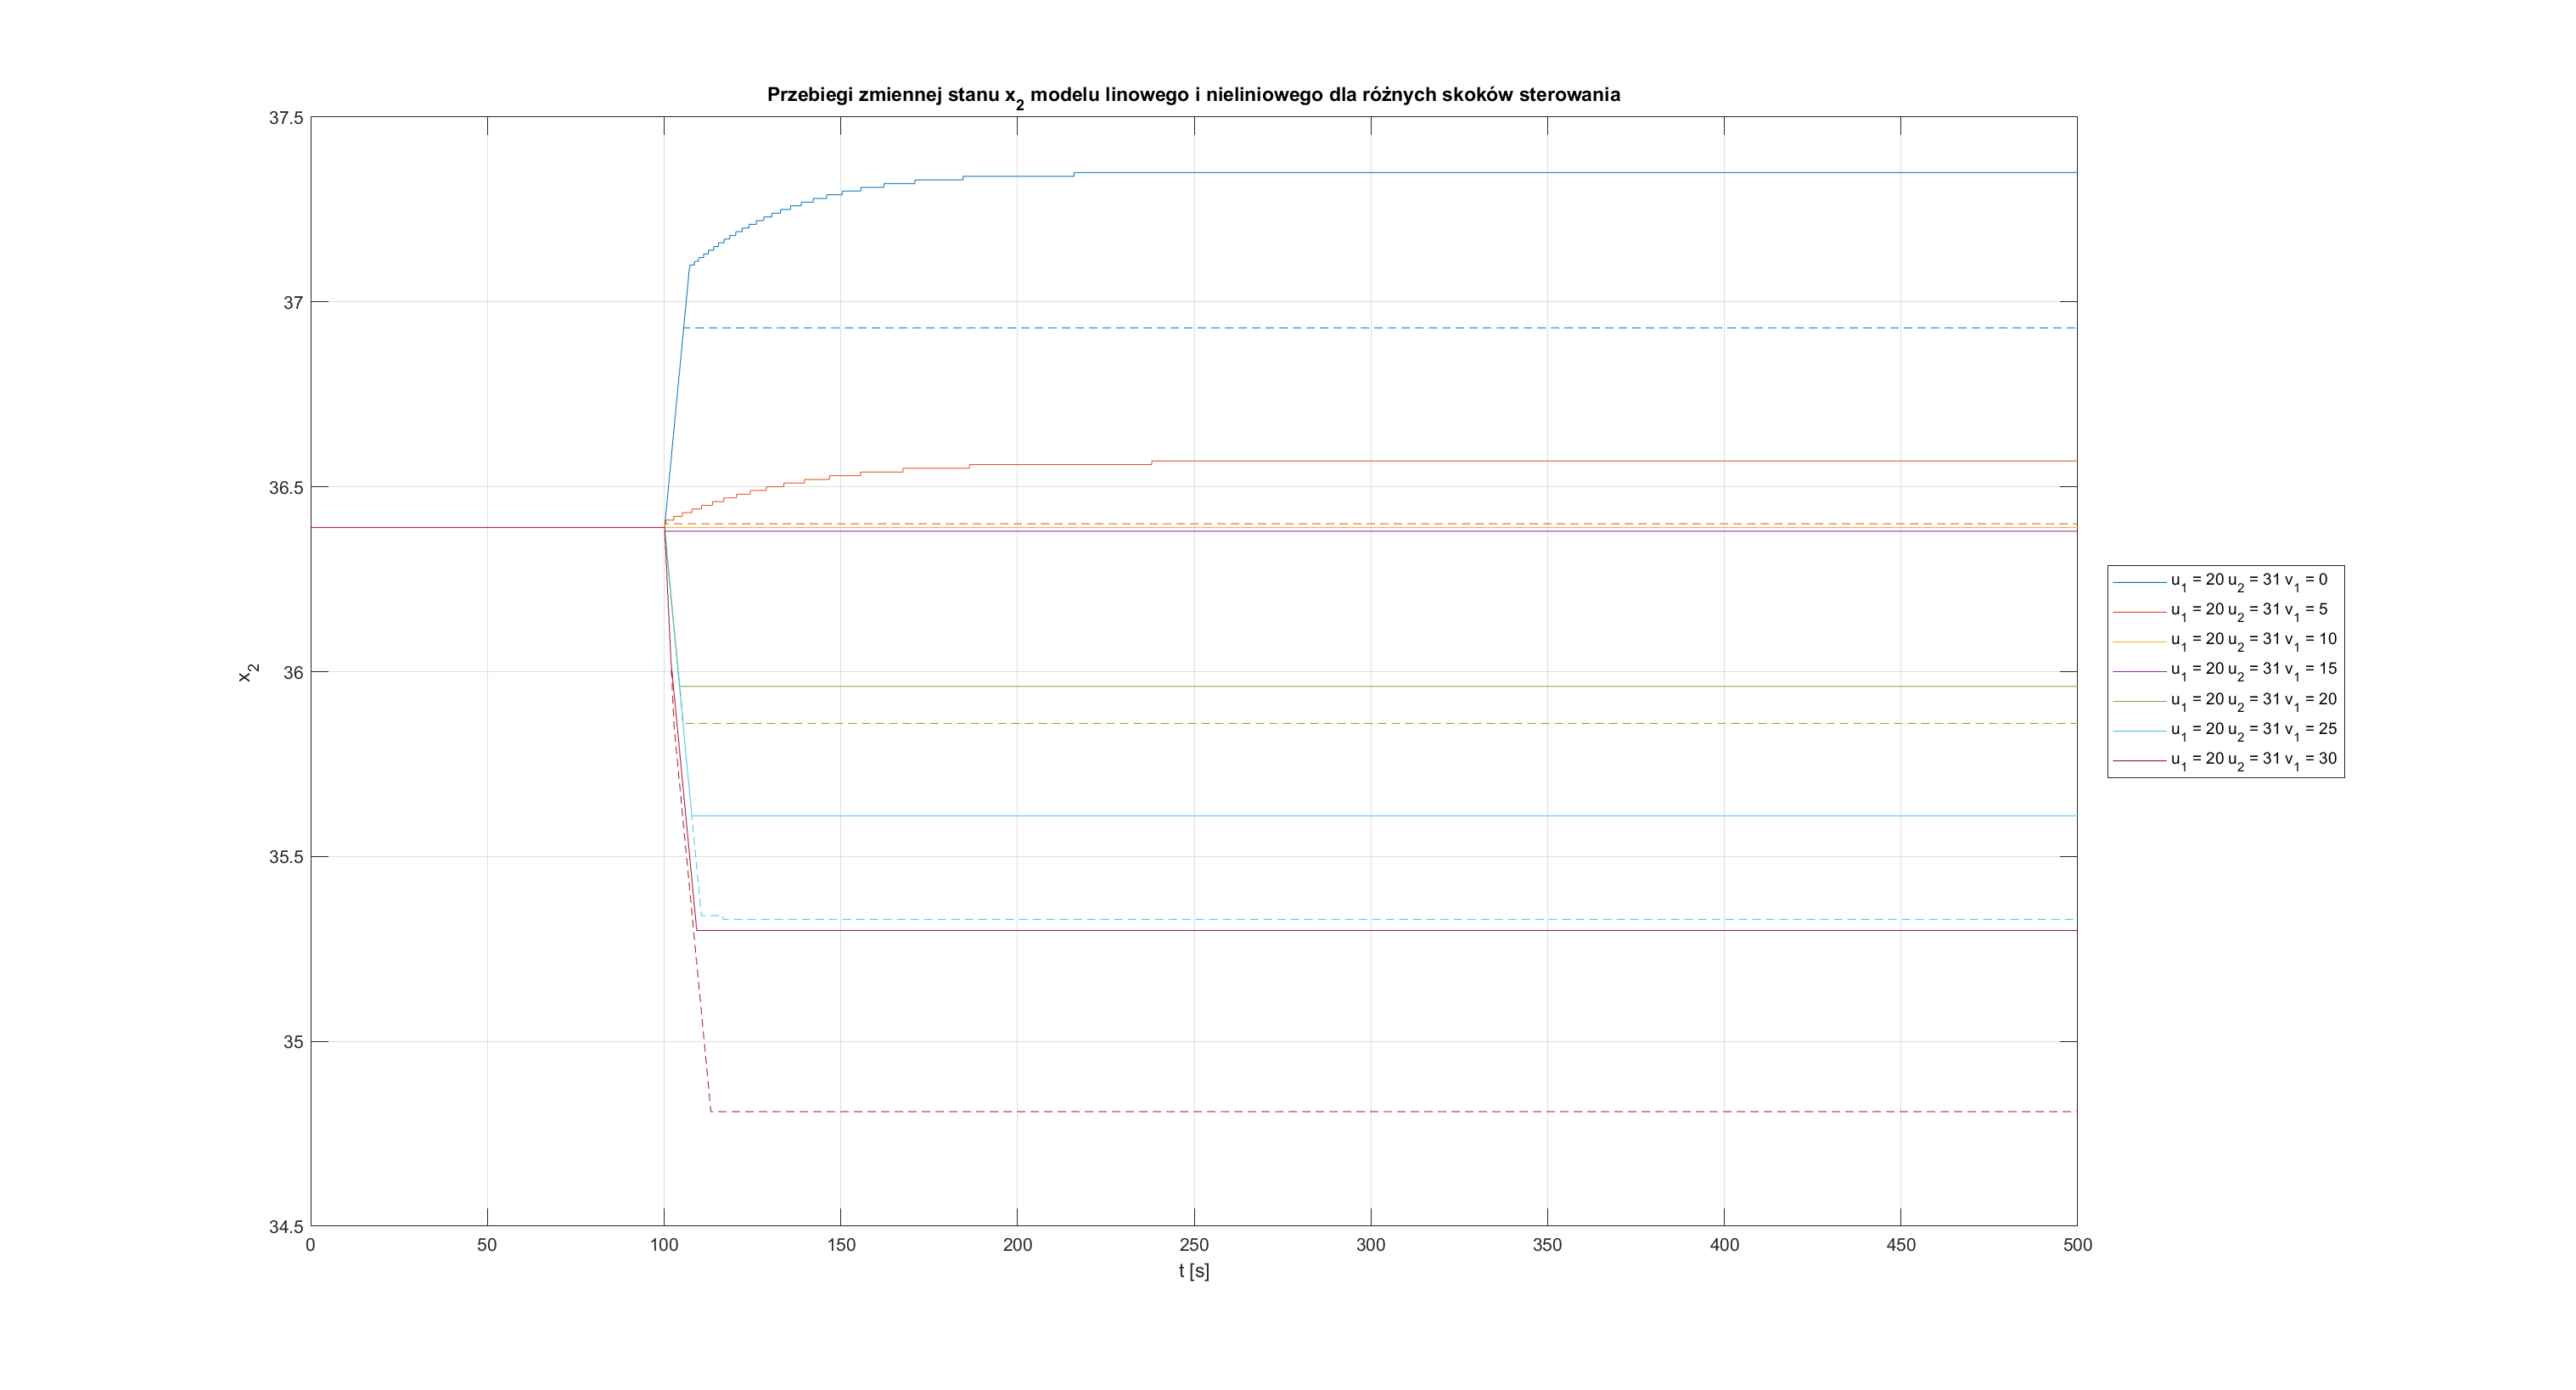
\includegraphics[scale=0.35]{images/x2_u1=20_u2=31_v1=30_dt=0.1.eps}
    \caption{Porównanie modeli liniowych i nieliniowych}
\end{figure}

\begin{figure}[H]
    \centering
    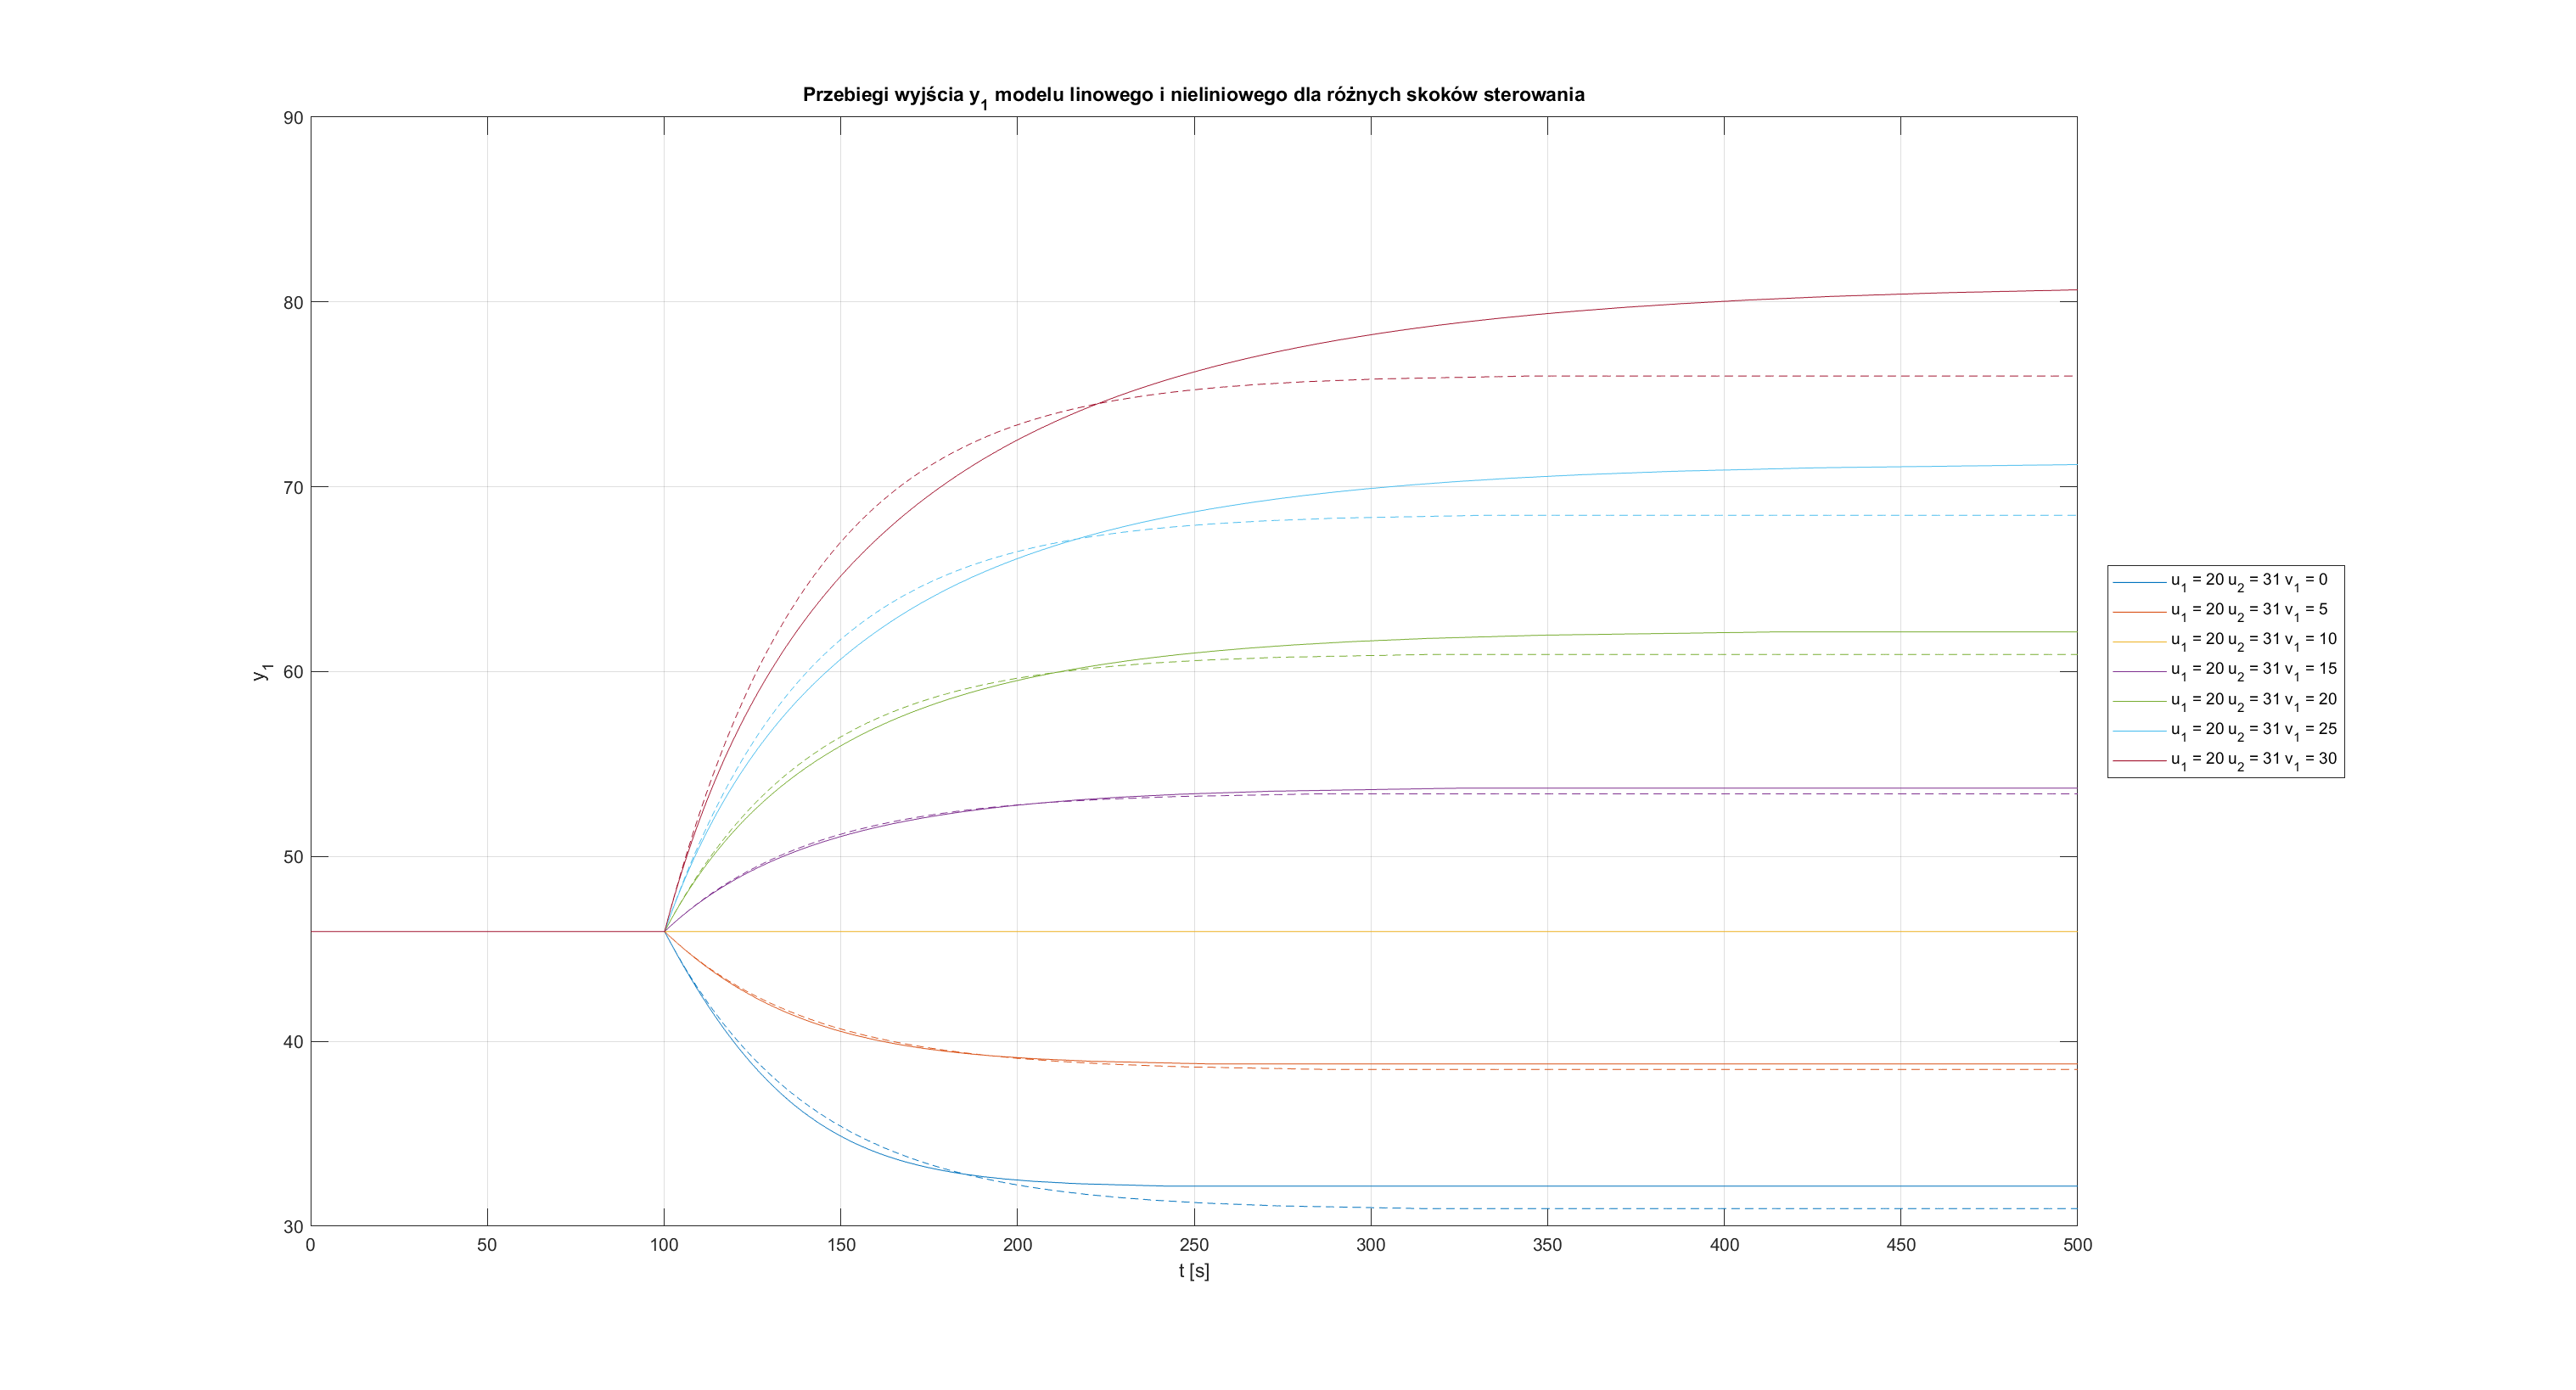
\includegraphics[scale=0.35]{images/y1_u1=20_u2=31_v1=30_dt=0.1.eps}
    \caption{Porównanie modeli liniowych i nieliniowych}
\end{figure}

\begin{figure}[H]
    \centering
    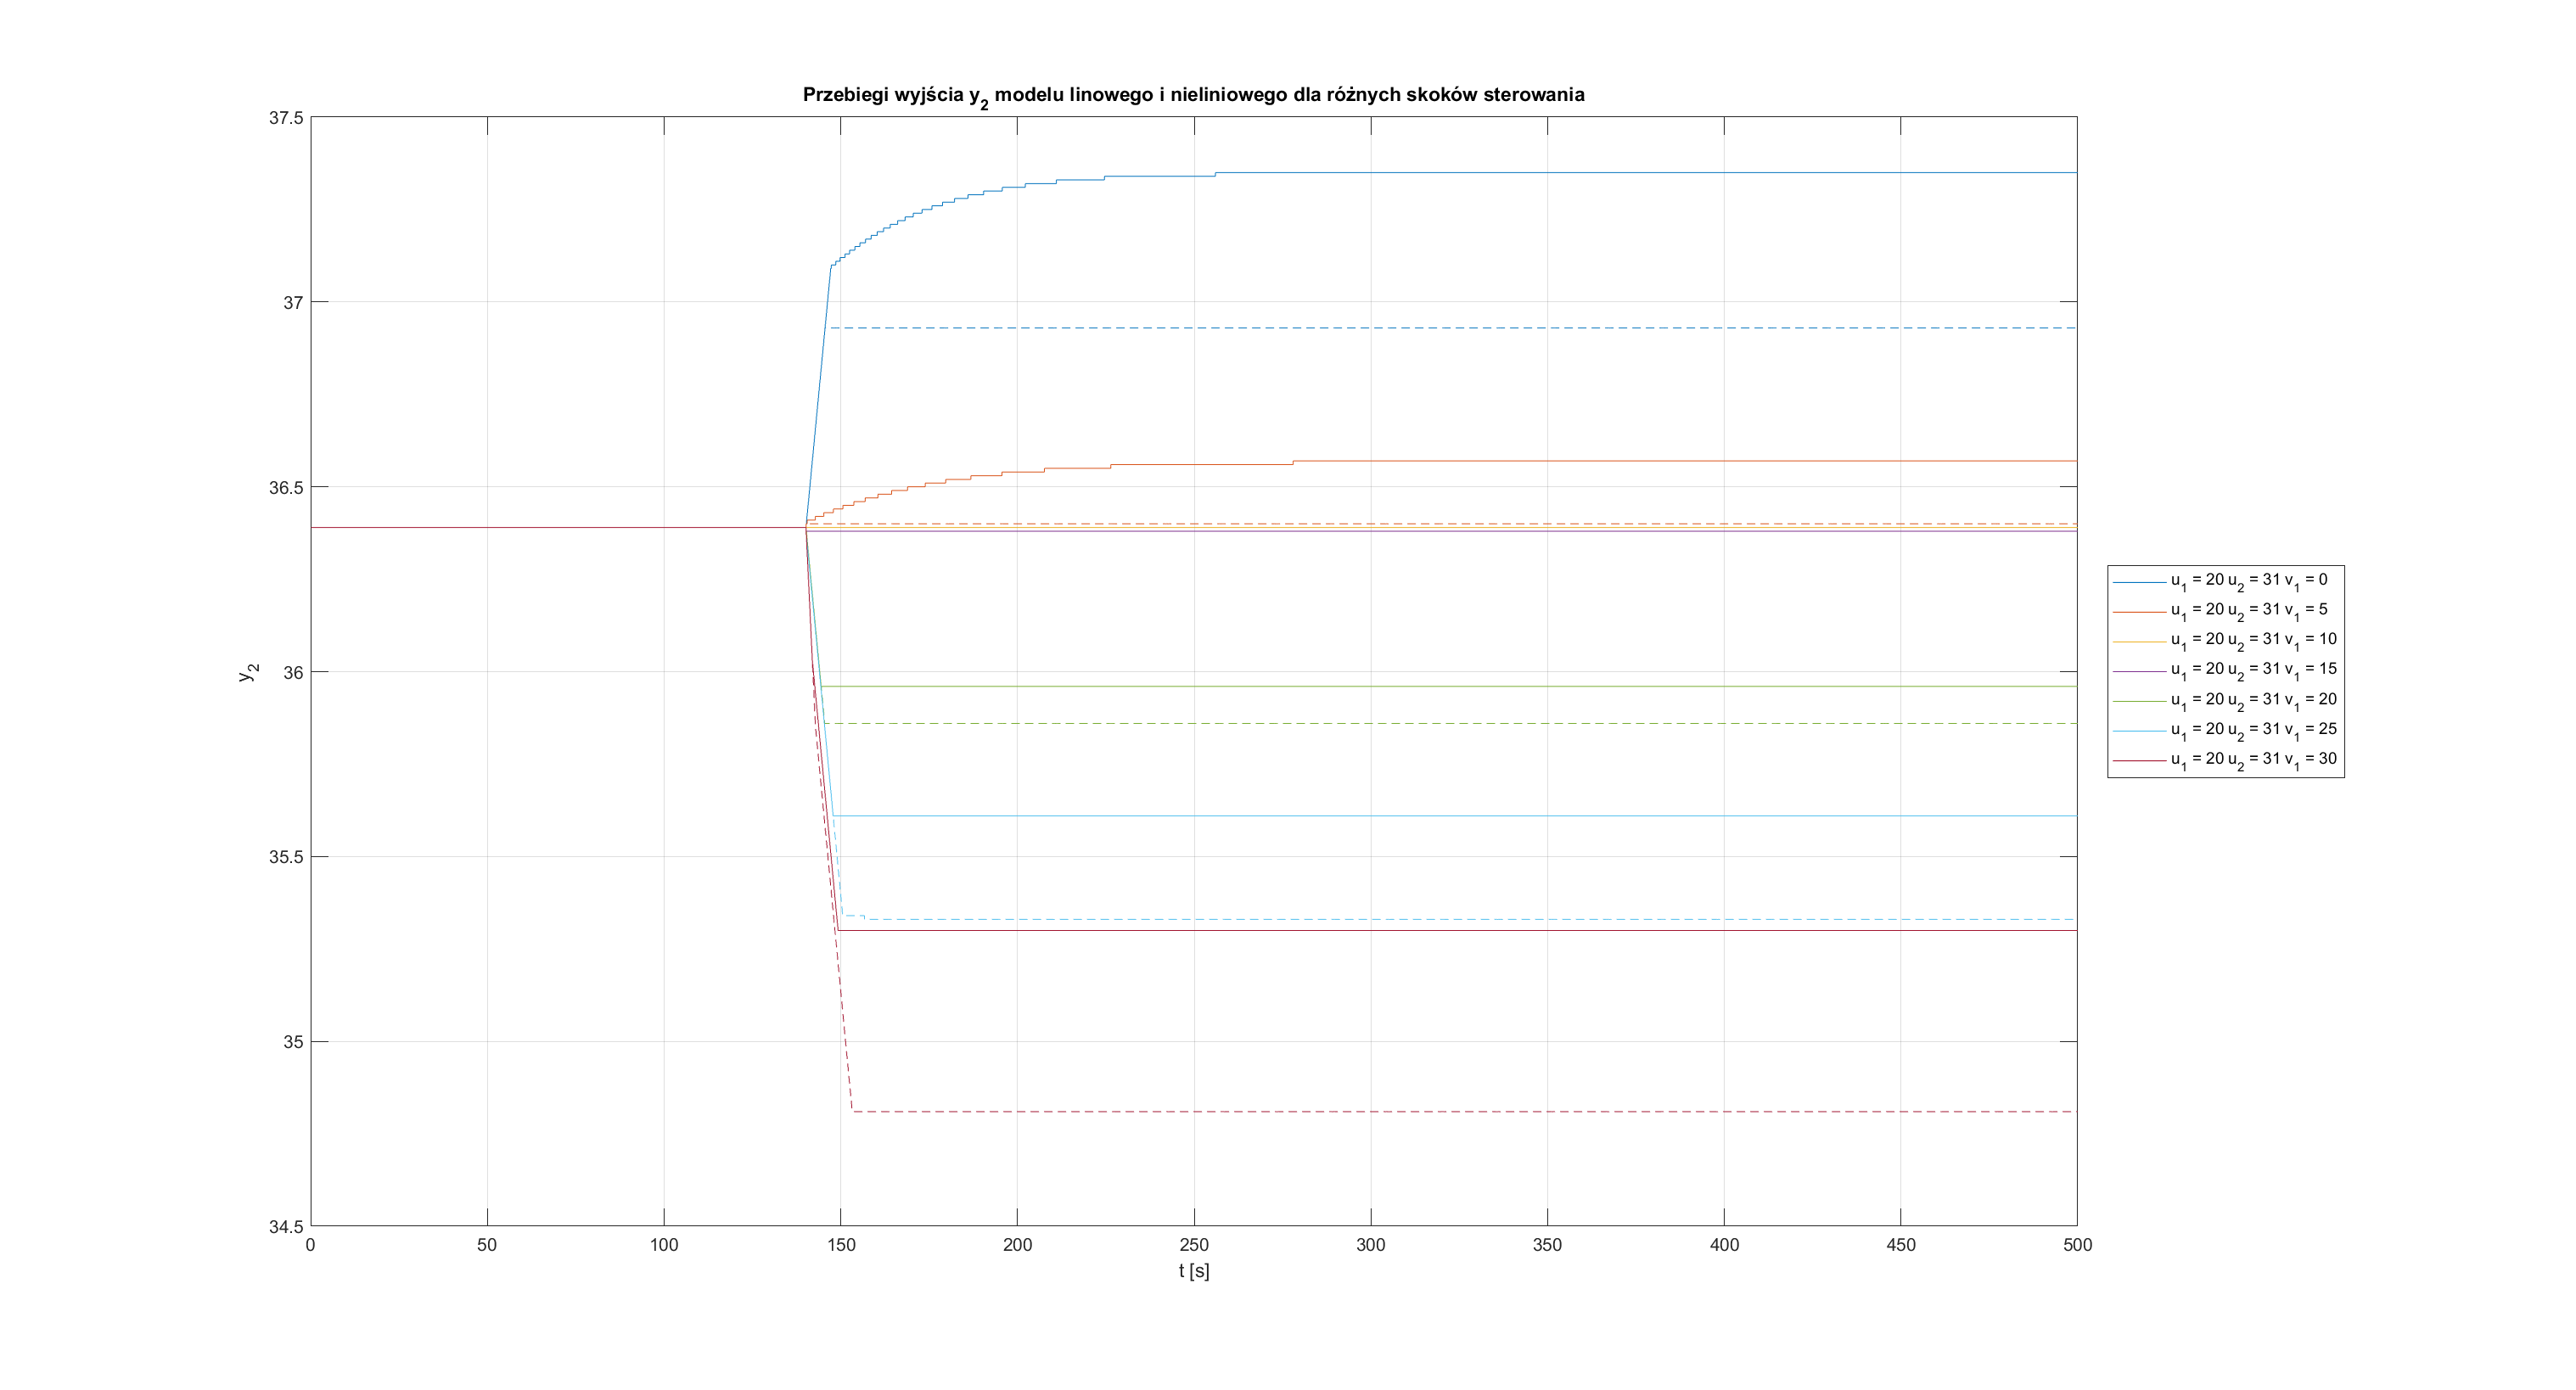
\includegraphics[scale=0.35]{images/y2_u1=20_u2=31_v1=30_dt=0.1.eps}
    \caption{Porównanie modeli liniowych i nieliniowych}
\end{figure}

W ostatnim eksperymencie zmieniano wszystkie wejścia naraz.

\begin{figure}[H]
    \centering
    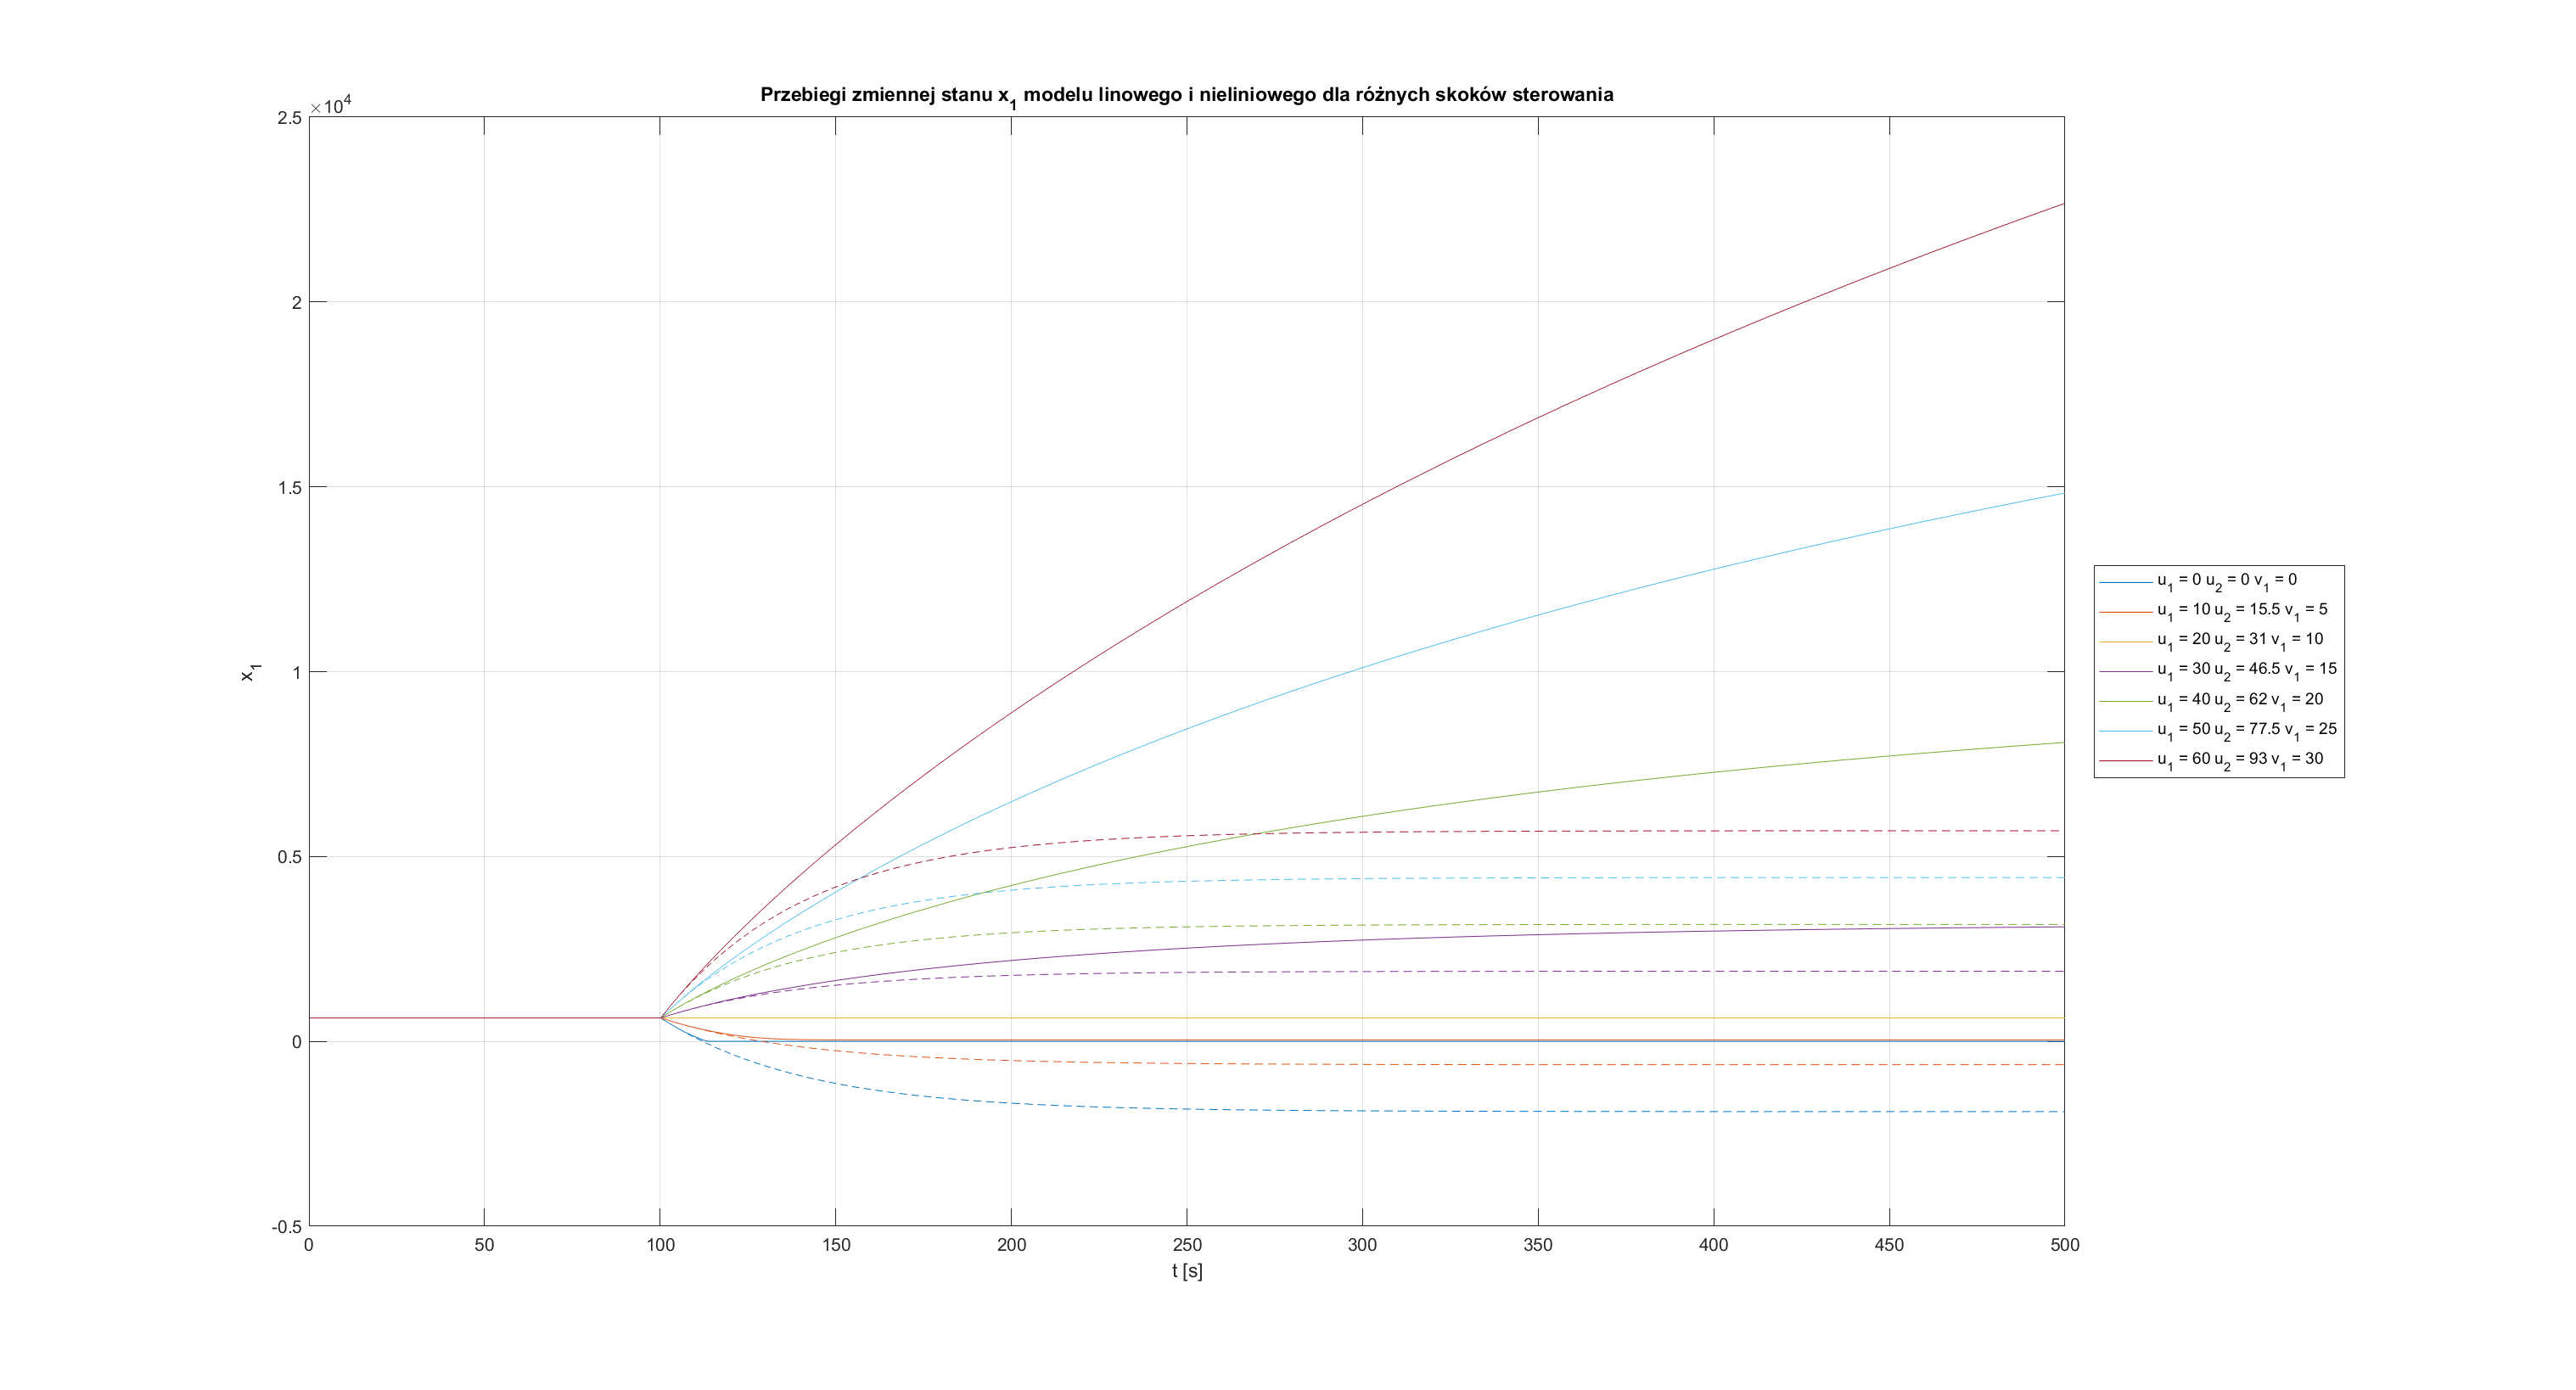
\includegraphics[scale=0.35]{images/x1_u1=60_u2=93_v1=30_dt=0.1.eps}
    \caption{Porównanie modeli liniowych i nieliniowych}
\end{figure}

\begin{figure}[H]
    \centering
    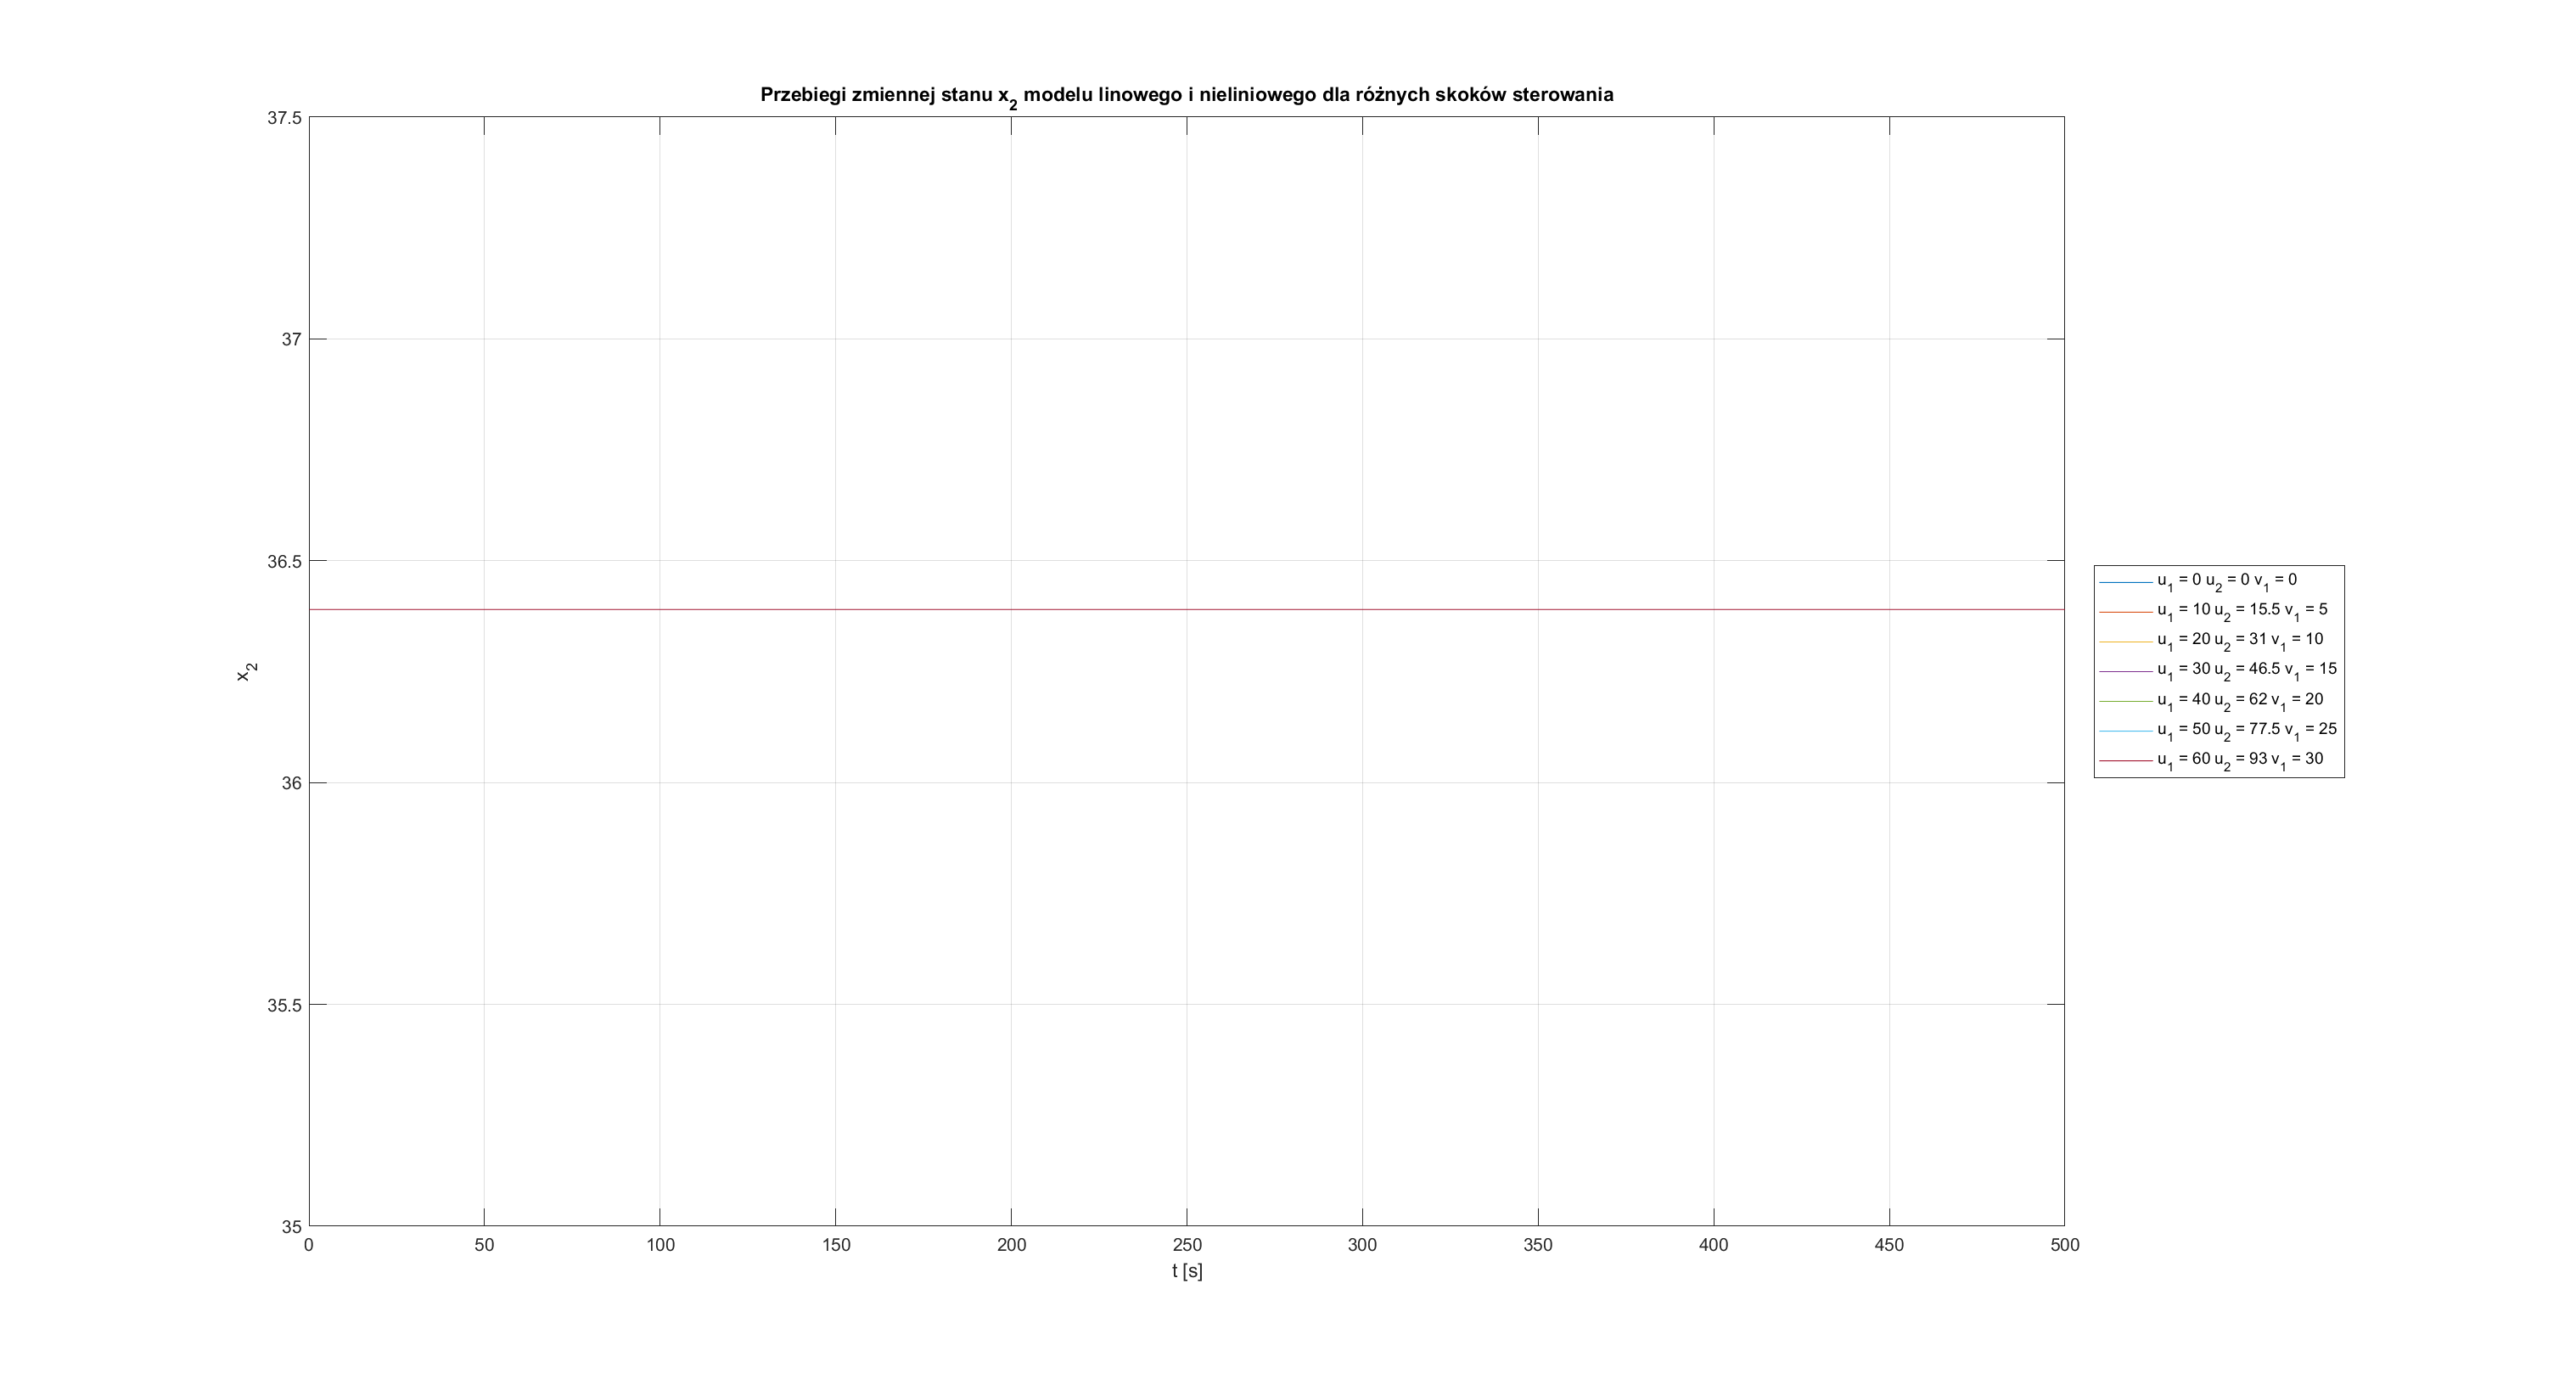
\includegraphics[scale=0.35]{images/x2_u1=60_u2=93_v1=30_dt=0.1.eps}
    \caption{Porównanie modeli liniowych i nieliniowych}
\end{figure}

\begin{figure}[H]
    \centering
    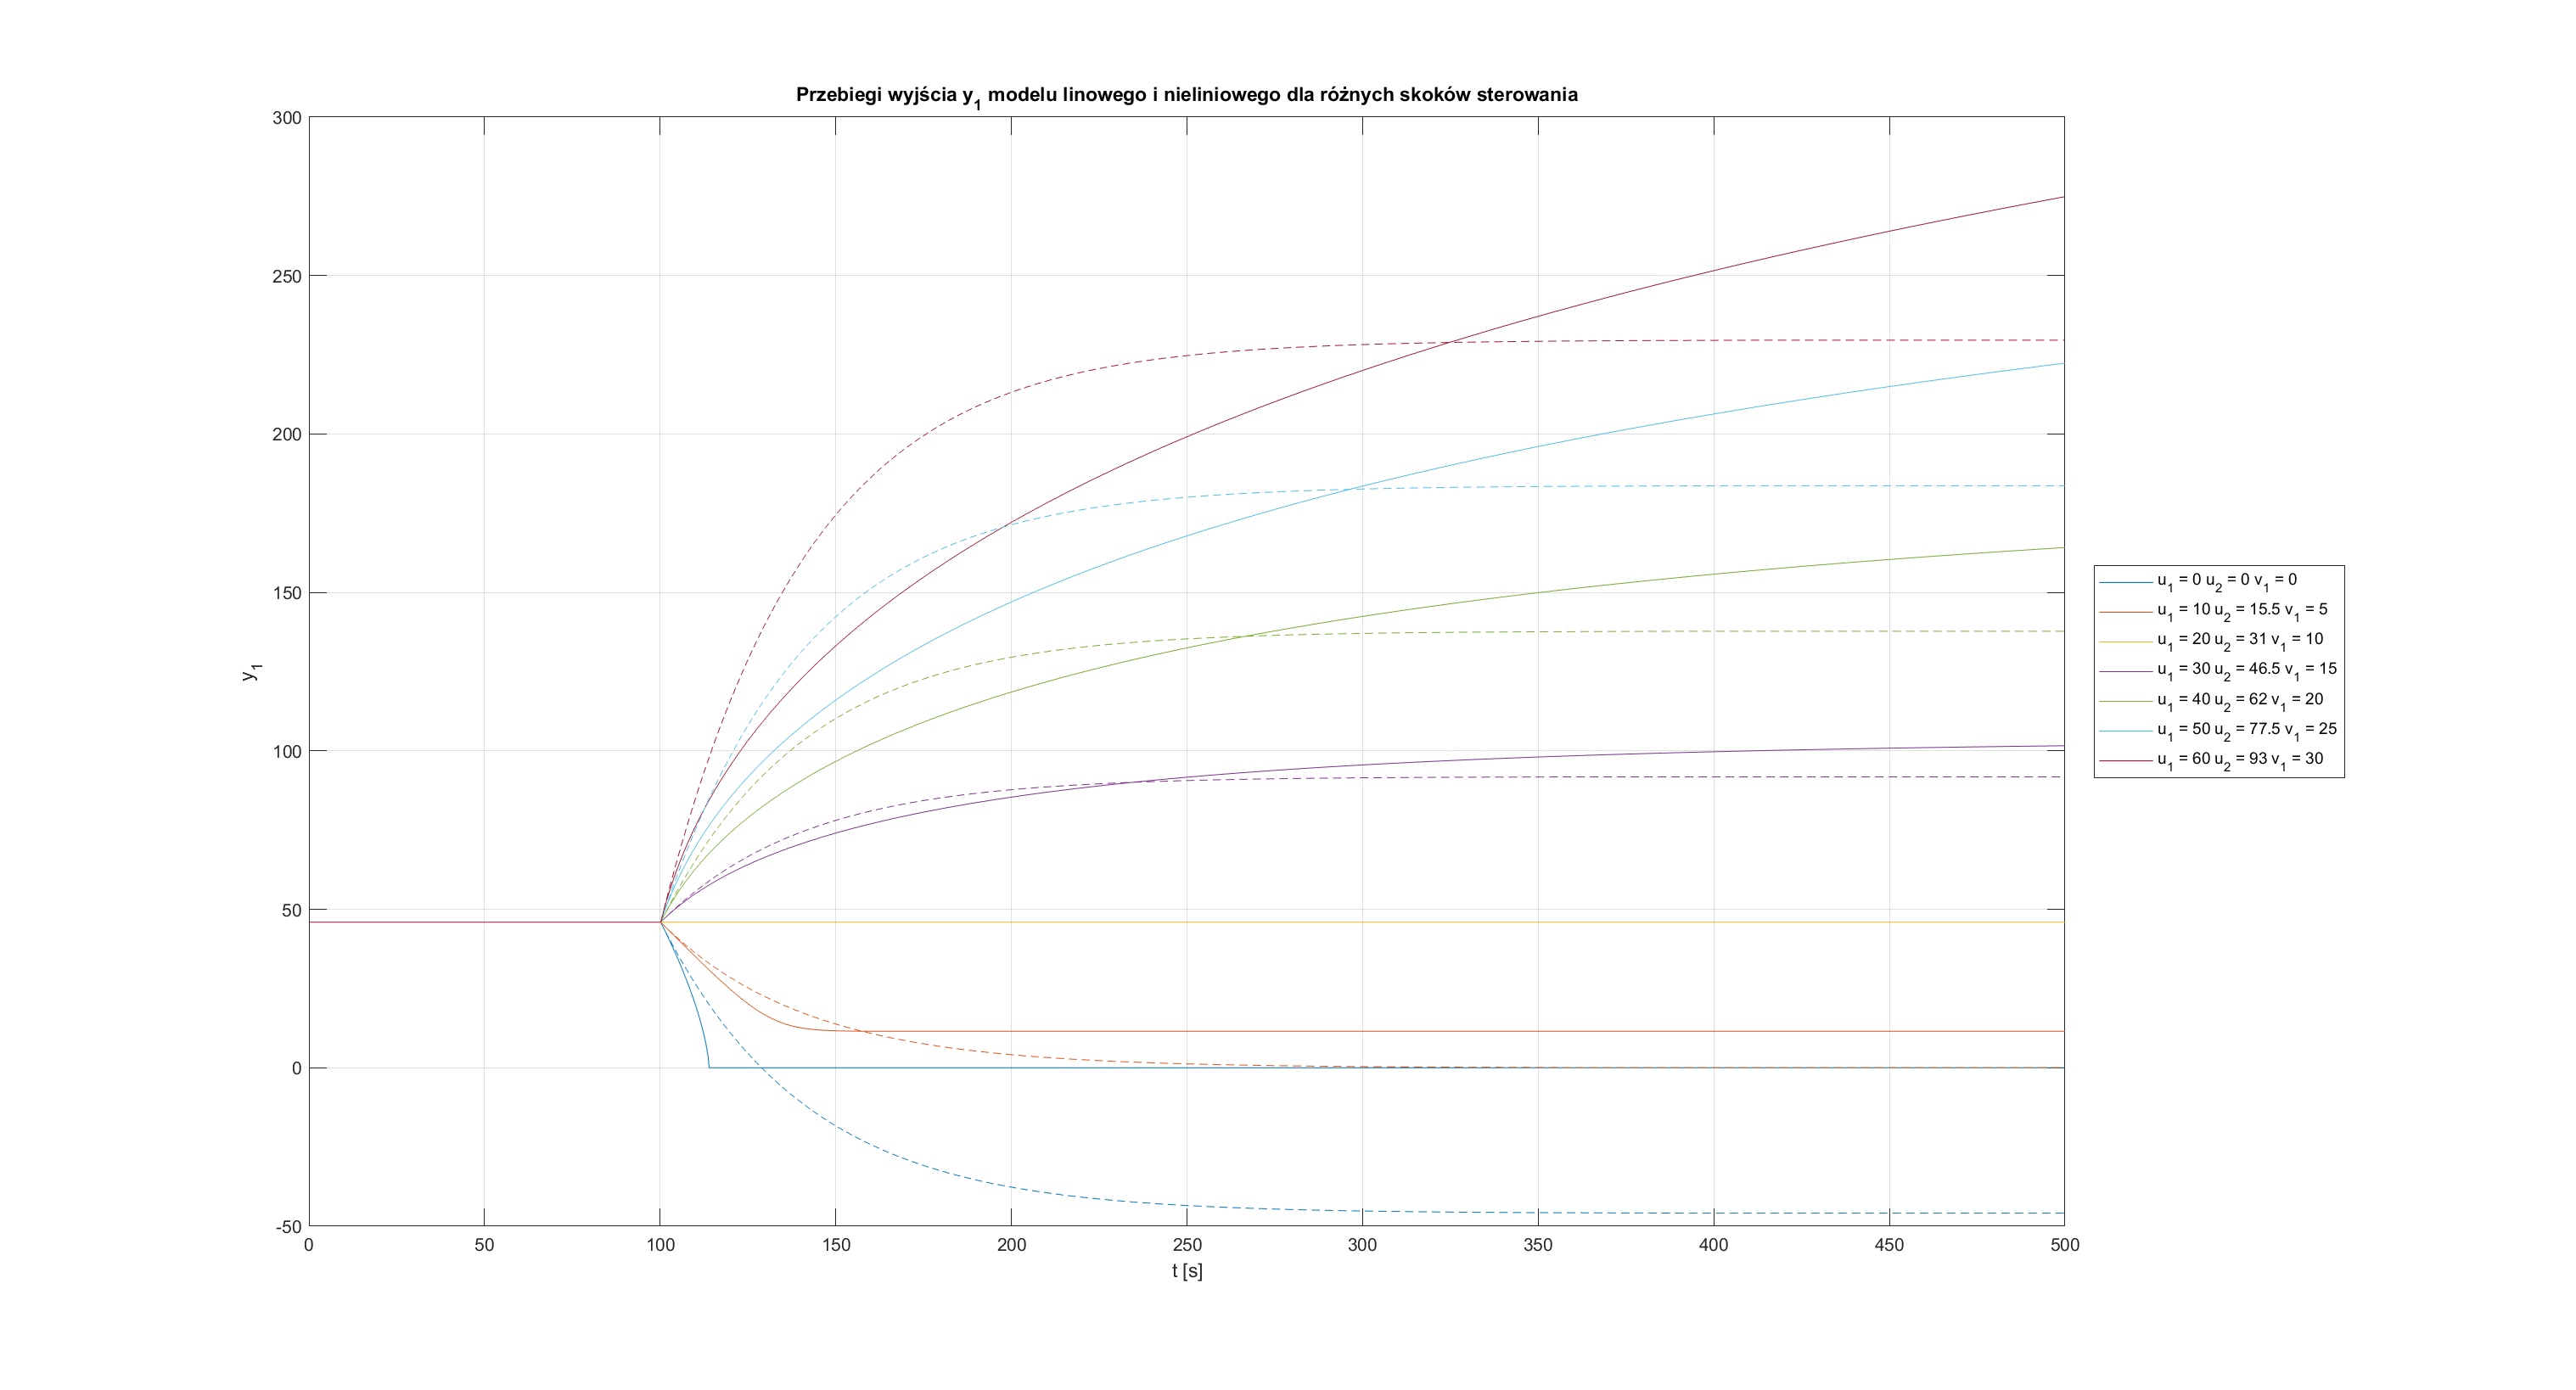
\includegraphics[scale=0.35]{images/y1_u1=60_u2=93_v1=30_dt=0.1.eps}
    \caption{Porównanie modeli liniowych i nieliniowych}
\end{figure}

\begin{figure}[H]
    \centering
    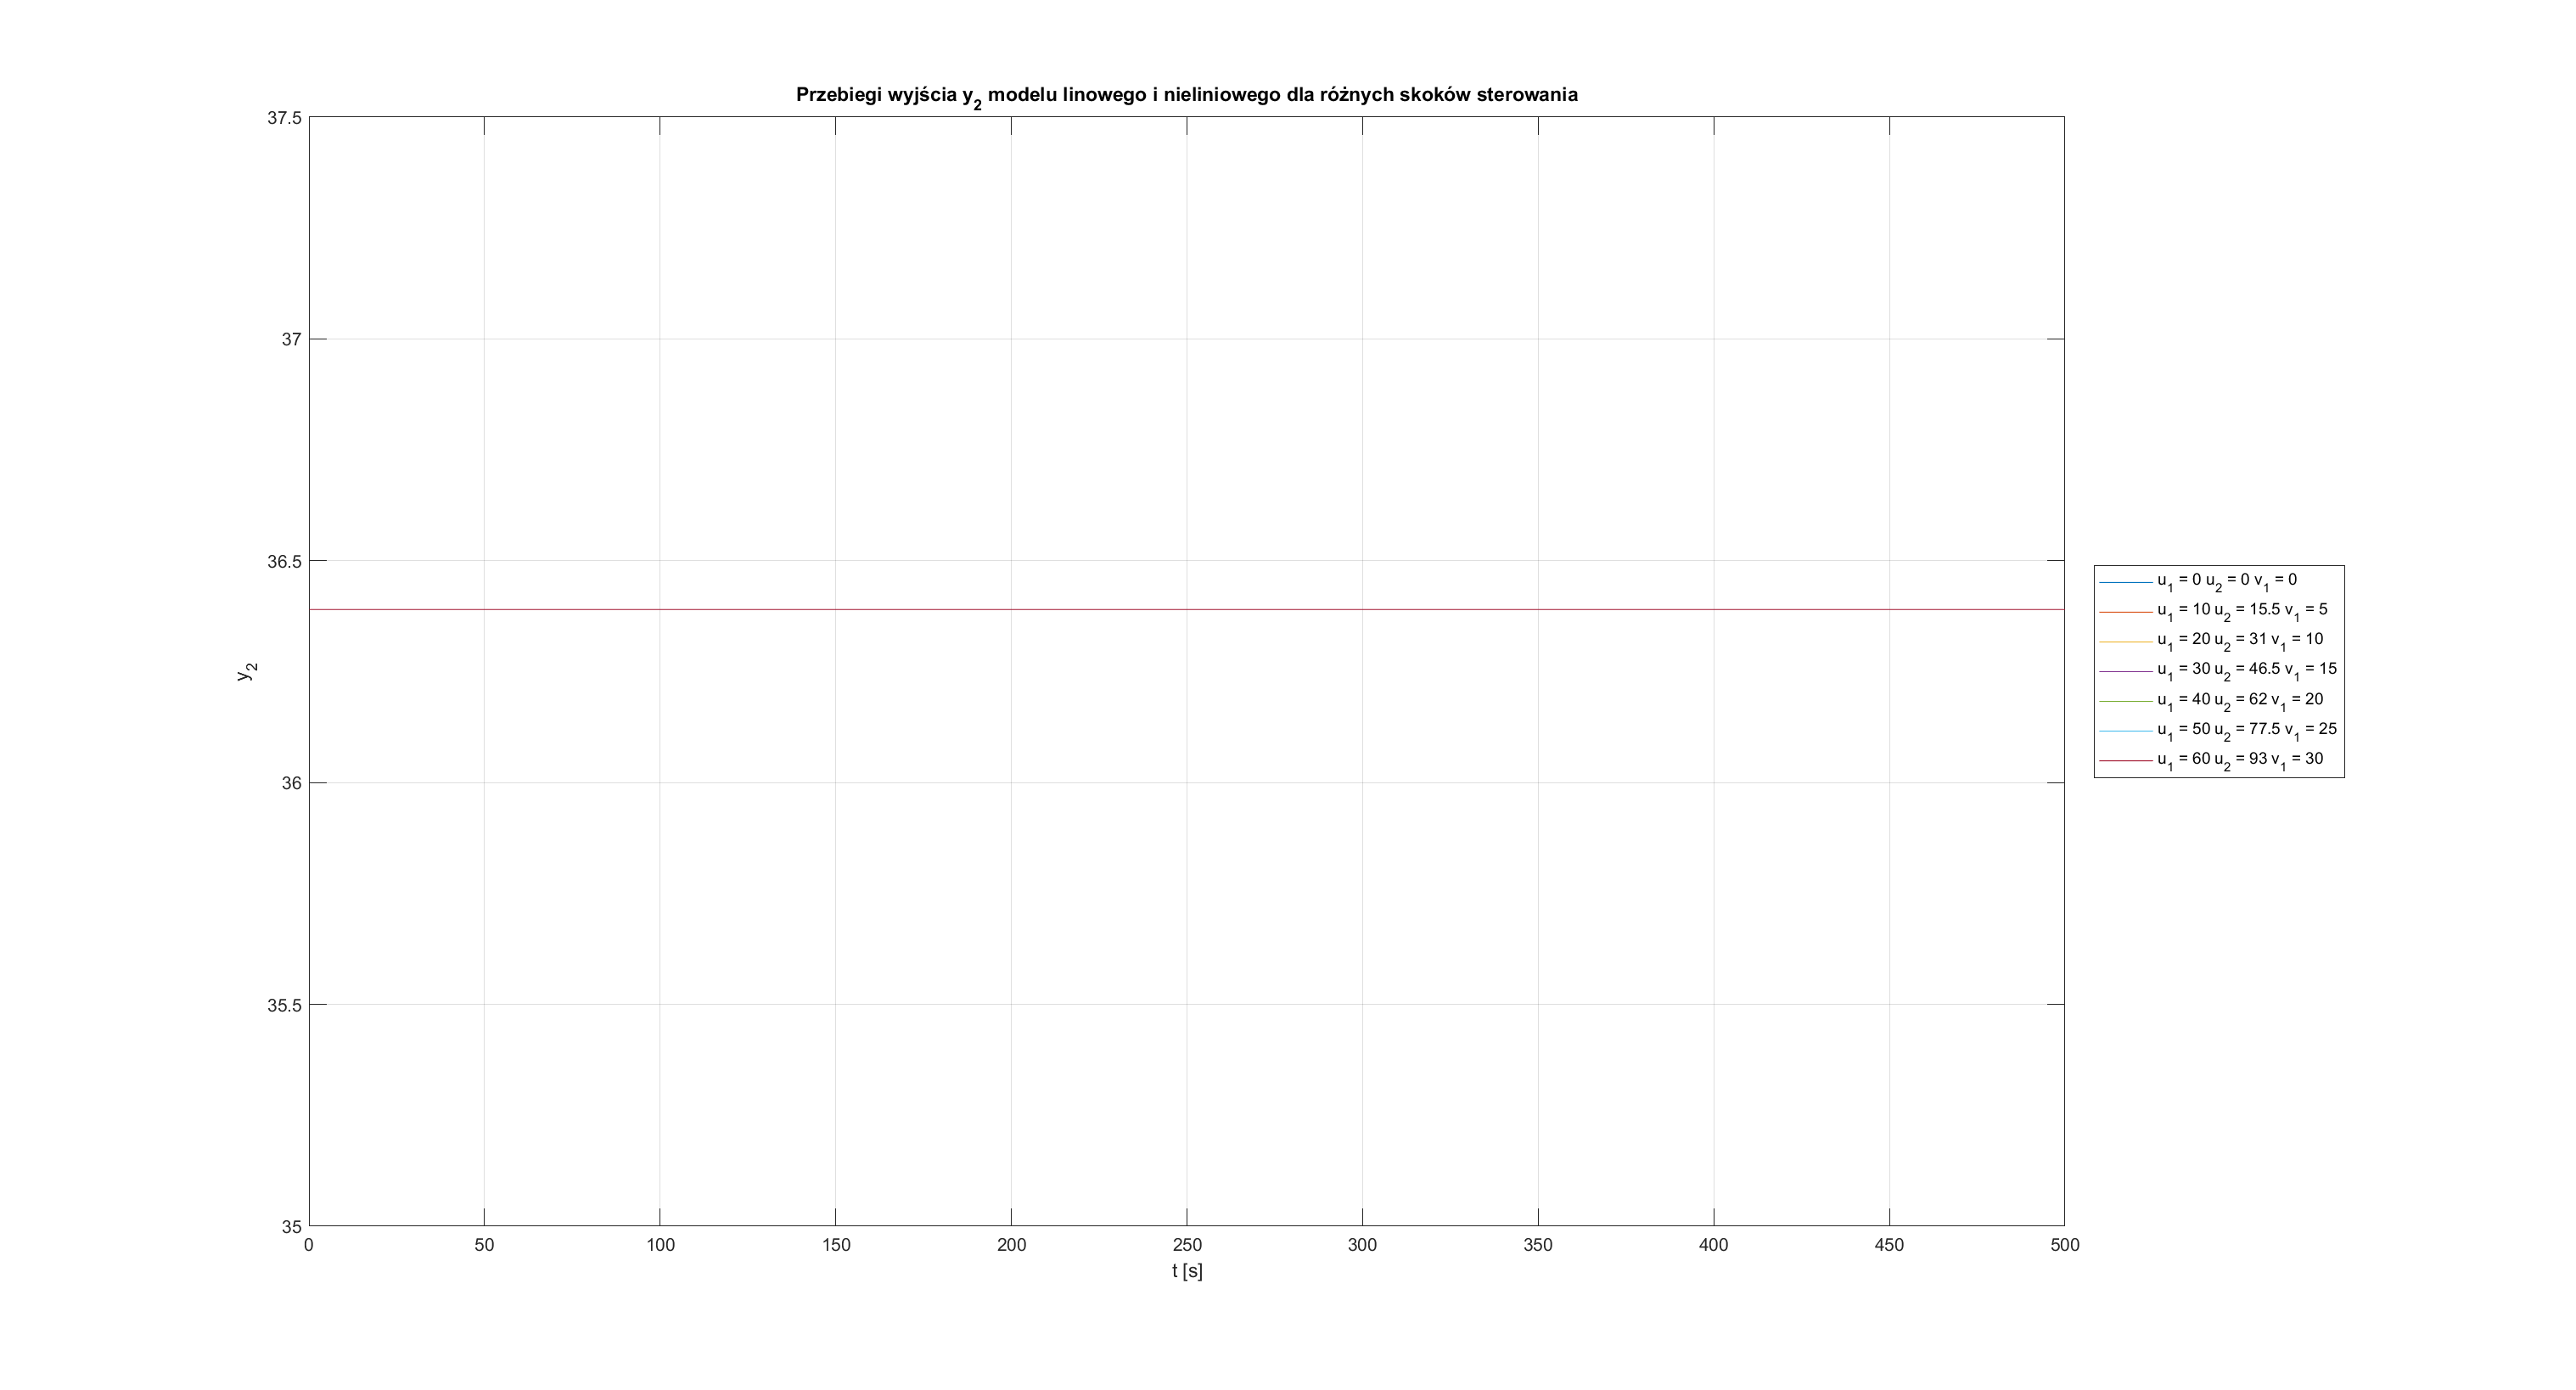
\includegraphics[scale=0.35]{images/y2_u1=60_u2=93_v1=30_dt=0.1.eps}
    \caption{Porównanie modeli liniowych i nieliniowych}
\end{figure}

Wniosek:
Wraz z oddaleniem się wejść oraz zakłócenia od parametrów zadanych przybliżenie modelu modelem liniowym stopniowo traci sens, gdyż wyniki zbyt znacząco się rozbiegają.
\newpage
\section{Dyskusja na temat jakości przybliżenia liniowego}
W przedstawionych w poprzednim podpunkcie wykresach można łatwo zauważyć, że jakość przybliżenia liniowego jest zależna od odległości od punktu pracy. Gdy odległość ta nie jest zbyt duża przybliżenie dostarcza w miarę sensowne rezultaty, mogące mieć późniejsze zastosowania. Jednakże, jeśli zadane wejście oddali się znacząco od punktu pracy wyniki bardzo rozbiegają się od modelu nieliniowego, można stwierdzić, że model liniowy nie nadaje się do ich sensownego przybliżania.

% wez tez napisz dwa slowa ze te wykresy zostaly zrobione na podstawie przeklepanych z reki dyskretnych rownan stanu do matlaba



\newpage
\section{Modele dyskretne}
\subsection{Równania stanu}
Na podstawie modelu ciągłego opracowano następujący model dyskretny:
\begin{align*}
 x_1(k)= &\left[ u_1(k-1) + u_2(k-1-\frac{\tau_c}{T_p}) + v_1(k-1) - \alpha \left( \frac{x_1(k-1)}{C} \right)^{0.25} \right]T_p +x_1(k-1)\\
\begin{split} x_2(k) =& 
 \bigg[ T_H \cdot u_1(k-1) + T_C \cdot u_2(k-1-\frac{\tau_c}{T_p}) + T_D \cdot v_1(k-1) +\\ & -\left( u_1(k-1) + u_2(k-1-\frac{\tau_c}{T_p}) + v_1(k-1) \right)\cdot x_2(k-1) \bigg]T_p \cdot x_1^{-1} (k-1)  +x_2(k-1)\end{split} \\\\
 y_1(k) = &\sqrt{\frac{x_1}{C}} \\\\
 y_2(k) =  &x_2(k-\tau)
\end{align*}




Dokonano linearyzacji w punkcie pracy $p = (\overline{u_1}, \overline{u_2}, \overline{v_1}, \overline{x_1}, \overline{x_2} )$:

\begin{align*}
\begin{split}
x_1(k) = &\left[ \overline{u_1} + \overline{u_2} + \overline{v_1} - \alpha \left( \frac{\overline{x_1}}{C} \right)^{0.25} \right]T_p + \overline{x_1} + T_p \left( u_1(k-1) - \overline{u_1} \right) +T_p\left( u_2(k-1 - \frac{\tau_c}{T_p}) - \overline{u_2} \right)+ \\ &+ \left( - \alpha Tp \frac{\overline{x_1}^{0.25}}{4 C^{0.25} x_1 } +1 \right)(x_1(k-1) -\overline{x_1})
\end{split}\\
\begin{split}
x_2(k) = &\bigg( T_H \overline{u_1} + T_C \overline{u_2} + T_D \overline{v_1} - (\overline{u_1}+\overline{u_2}+\overline{v_1})\overline{x_2} \bigg)\overline{x_1}^{-1}T_p + \overline{x_2} + \frac{T_p(T_H-\overline{x_2})}{\overline{x_1}}(u_1(k-1)-\overline{u_1})  + \\ &+ \frac{T_p(T_C-\overline{x_2})}{\overline{x_1}}\left(u_2(k-1-\frac{\tau_c}{T_p})-\overline{u_2}\right)+
\frac{T_p(T_D-\overline{v_1})}{\overline{v_1}}(v_1(k-1)-\overline{v_1}) + \\ &-\frac{T_p}{\overline{x_1}^2}\left( T_H \overline{u_1} + T_C \overline{u_2} + T_D \overline{v_1} - (\overline{u_1}+\overline{u_2}+\overline{v_1})\overline{x_2} \right)(x_1(k-1)-\overline{x_1}) +\\ &+
\left(\frac{-T_p}{\overline{x_1}}(\overline{u_1}+\overline{u_2}+\overline{v_1}) +1\right)(x_2(k-1)-\overline{x_2}) 
\end{split}\\
y_1(k) = &\sqrt{\frac{\overline{x_1}}{C}}+\frac{1}{2\sqrt{\overline{x_1}C}}(x_1(k)-\overline{x_1})\\
y_2(k) = &  x_2(k-\tau)
\end{align*}

\newpage

\subsection{Transmitancje}
 Przyjęto czas próbkowania $T_p = 0.1s$, korzystając z uprzednio wyliczonego w Matlabie modelu ciągłego a także polecenia \emph{c2d()} wyliczono następujące transmitancje:
 
 \begin{align*}
\frac{U_1}{Y_1} &= \frac{0.003995}{z - 0.9976} \\
\frac{U_1}{Y_2} &= z^{-400} \cdot \frac{0.004516 z - 0.004506}{z^2 - 1.997 z + 0.9966} \\
\frac{U_2}{Y_1} &= z^{-1000}\frac{0.003995}{z - 0.9976} \\
\frac{U_2}{Y_2} &= z^{-1400} \cdot \frac{-0.002587 z + 0.002581}{z^2 - 1.997 z + 0.9966} \\
\frac{V_1}{Y_1} &= \frac{0.003995}{z - 0.9976} \\
\frac{V_1}{Y_2} &= z^{-400} \cdot \frac{-0.001009 z + 0.001006}{z^2 - 1.997 z + 0.9966} \\
 \end{align*}
 
\subsection{Porównanie modelu ciągłego z dyskretnym}

Zarejestrowano odpowiedzi skokowe modelu ciągłego i modeli dyskretnych o różnym czasie próbkowania. Wyniki tych doświadczeń przedstawiono na poniższych wykresach. 

\begin{figure}[H]
    \centering
    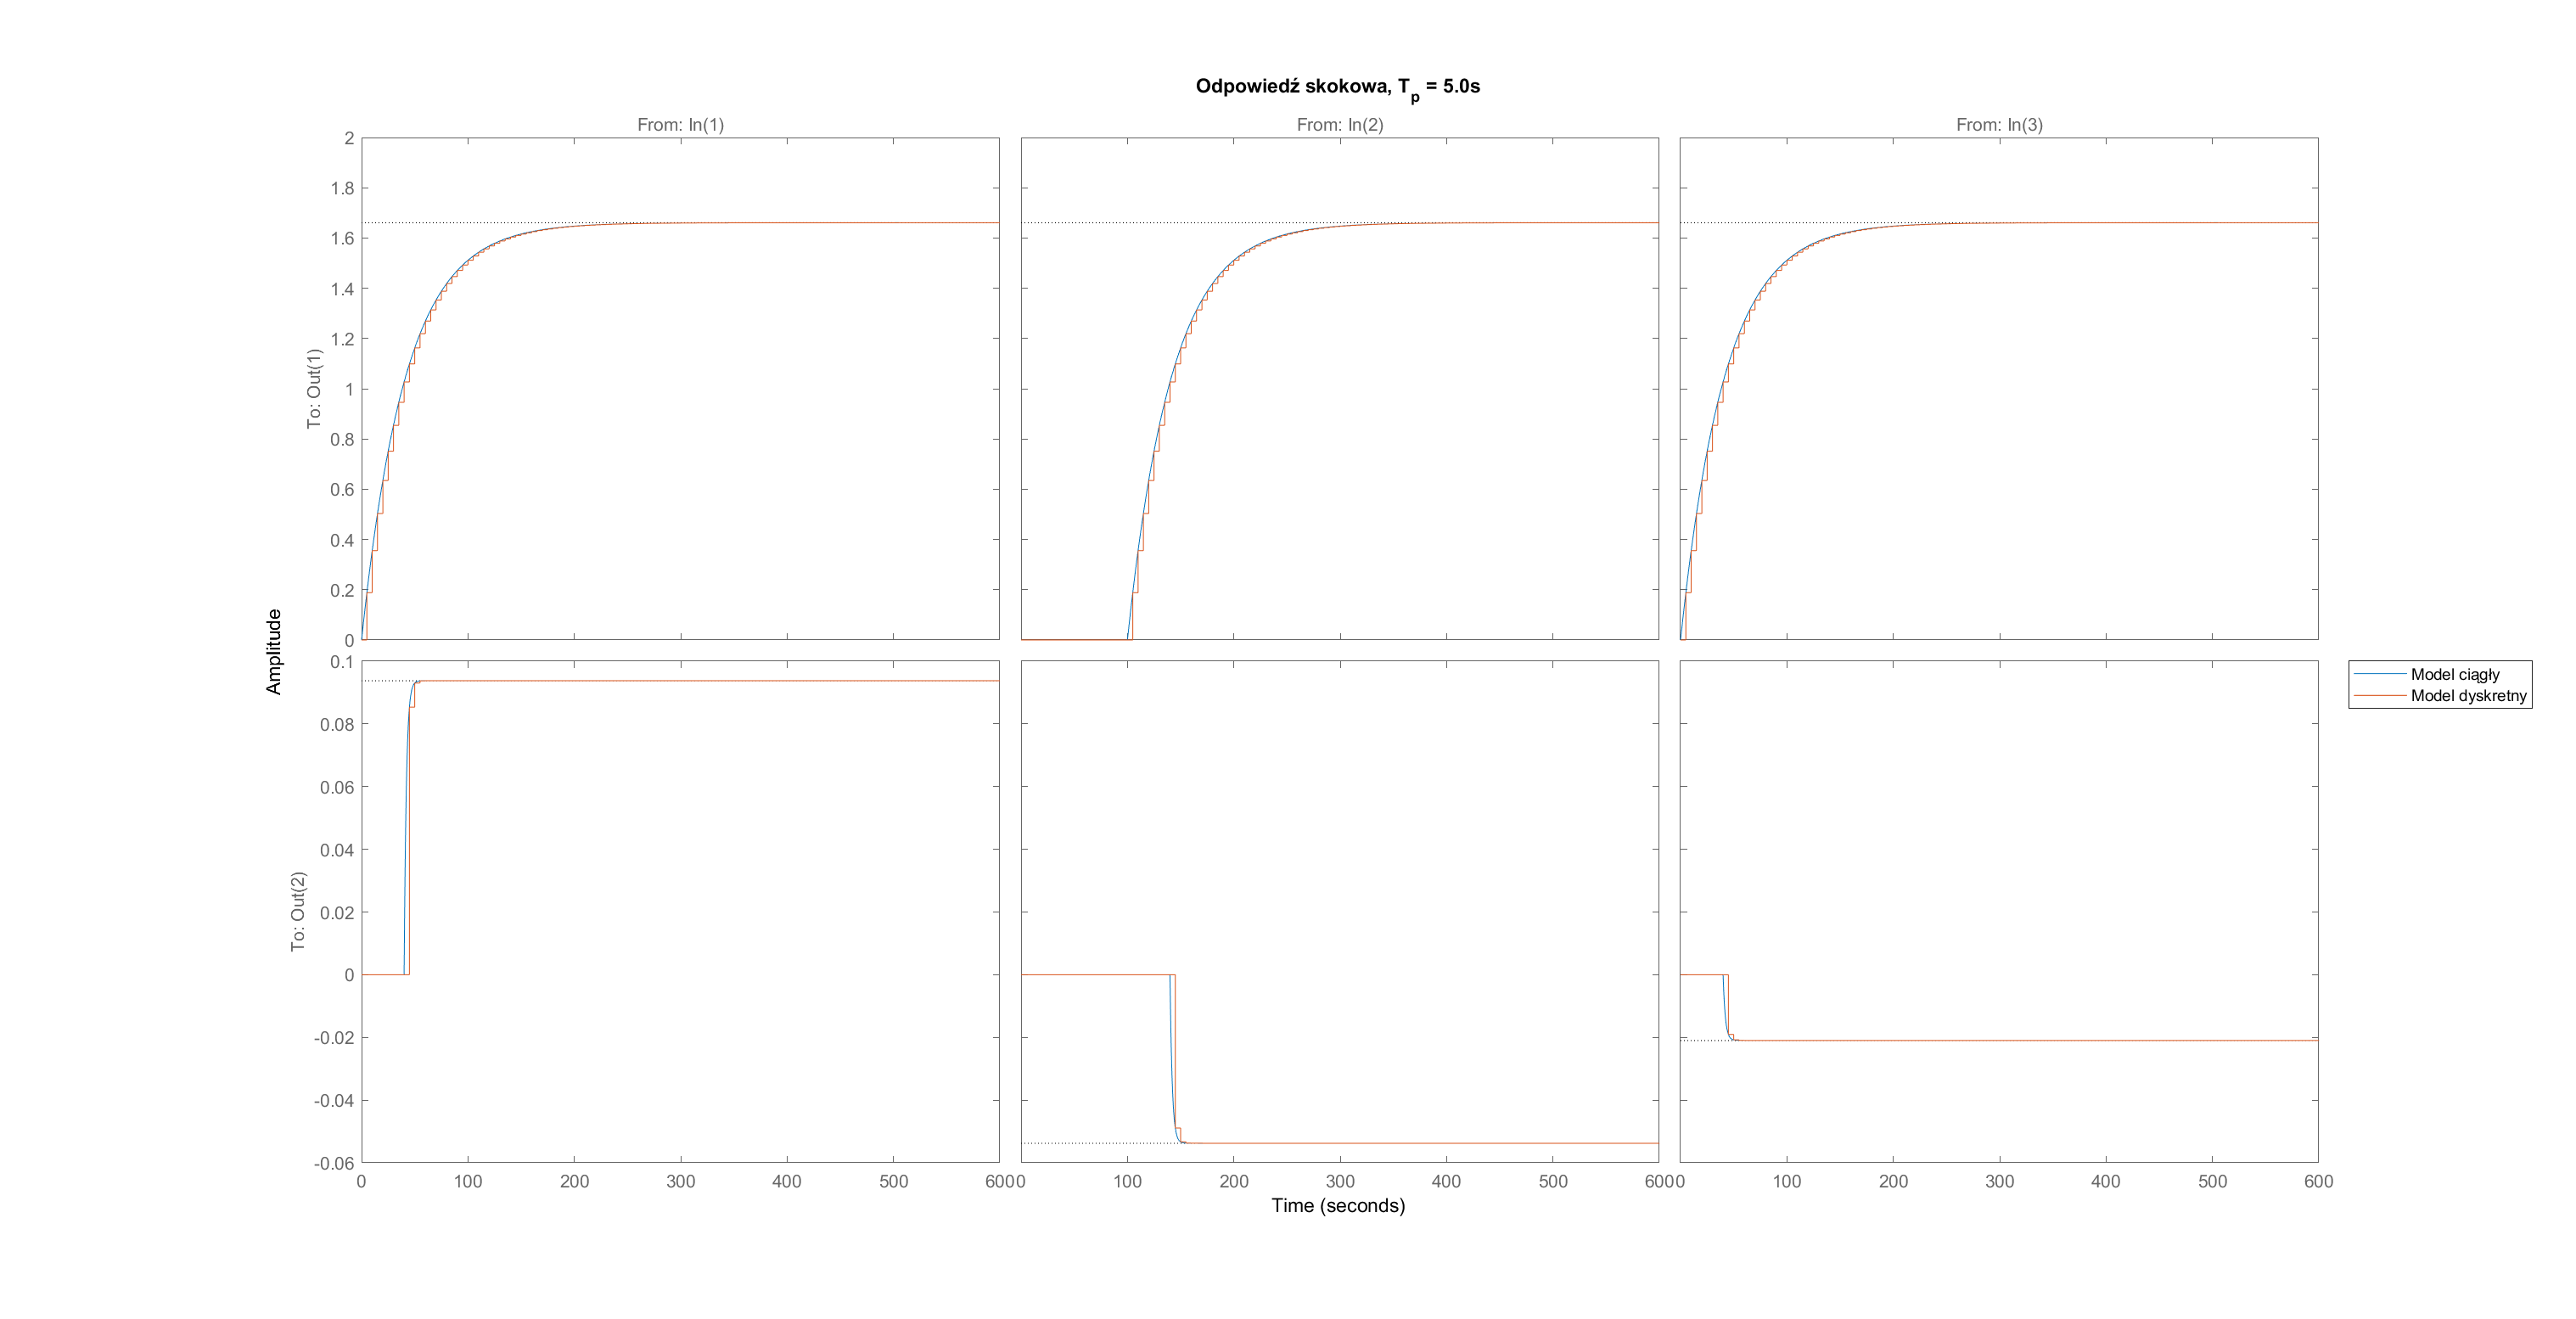
\includegraphics[scale=0.35]{images/stepdt5_00.eps}
    \caption{Odpowiedzi skokowe modeli}
\end{figure}

\begin{figure}[H]
    \centering
    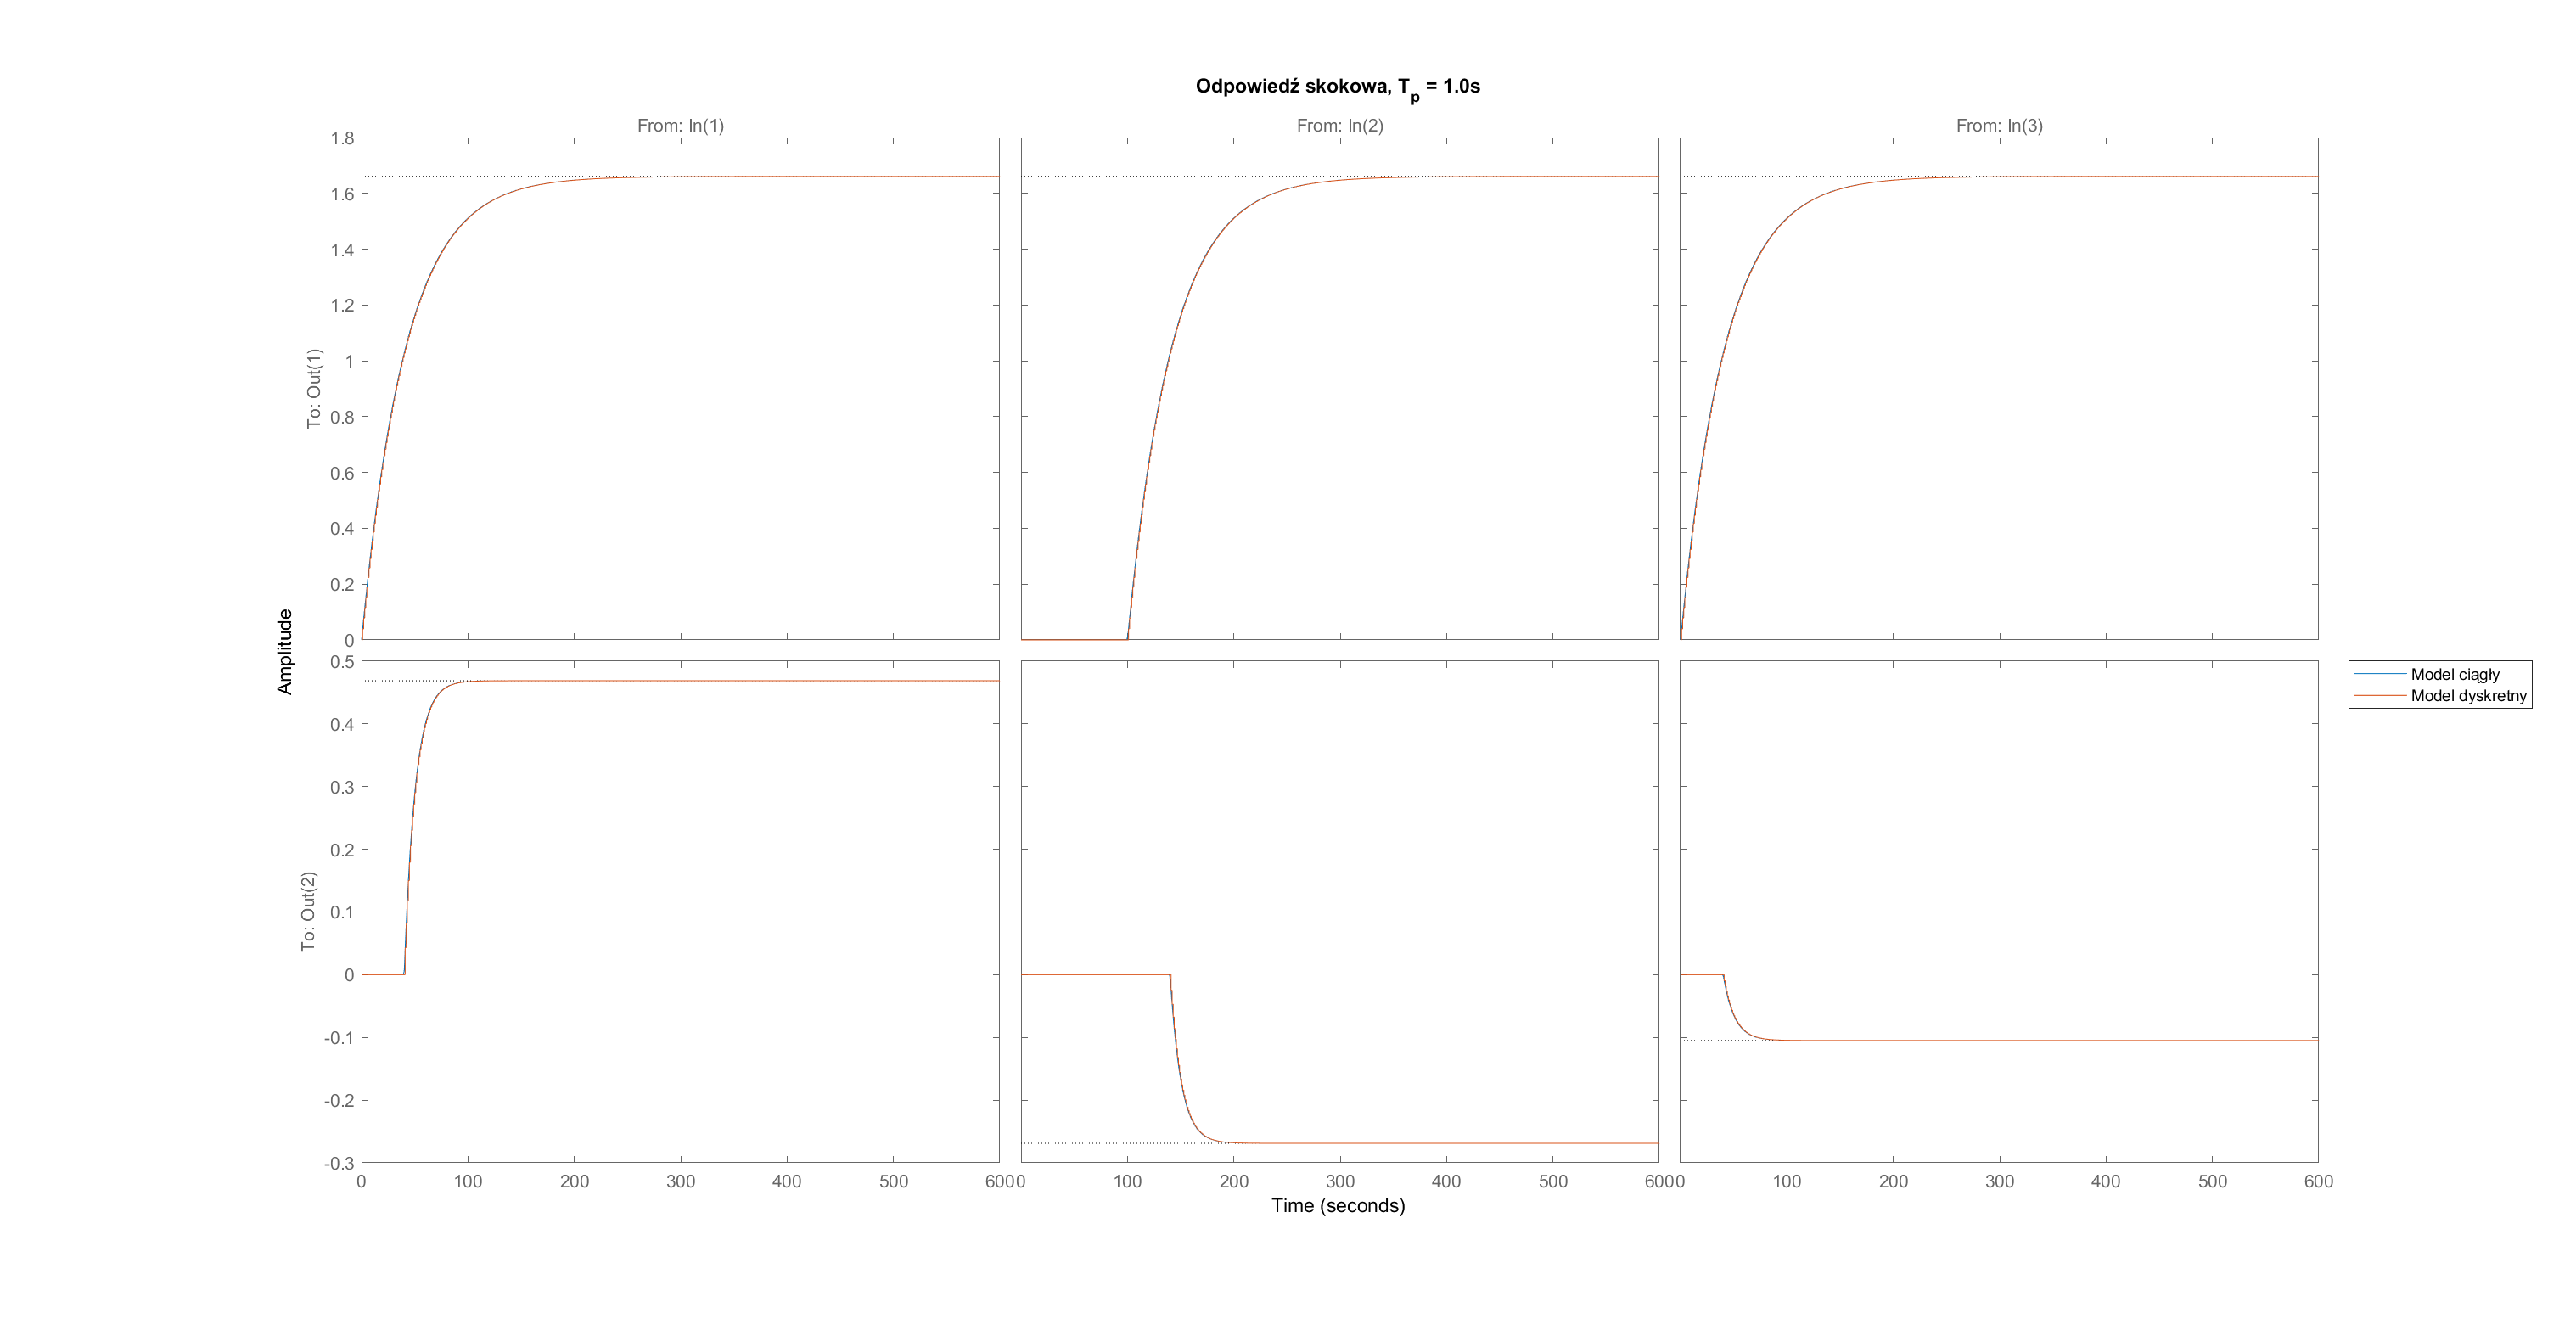
\includegraphics[scale=0.35]{images/stepdt1_00.eps}
    \caption{Odpowiedzi skokowe modeli}
\end{figure}

\begin{figure}[H]
    \centering
    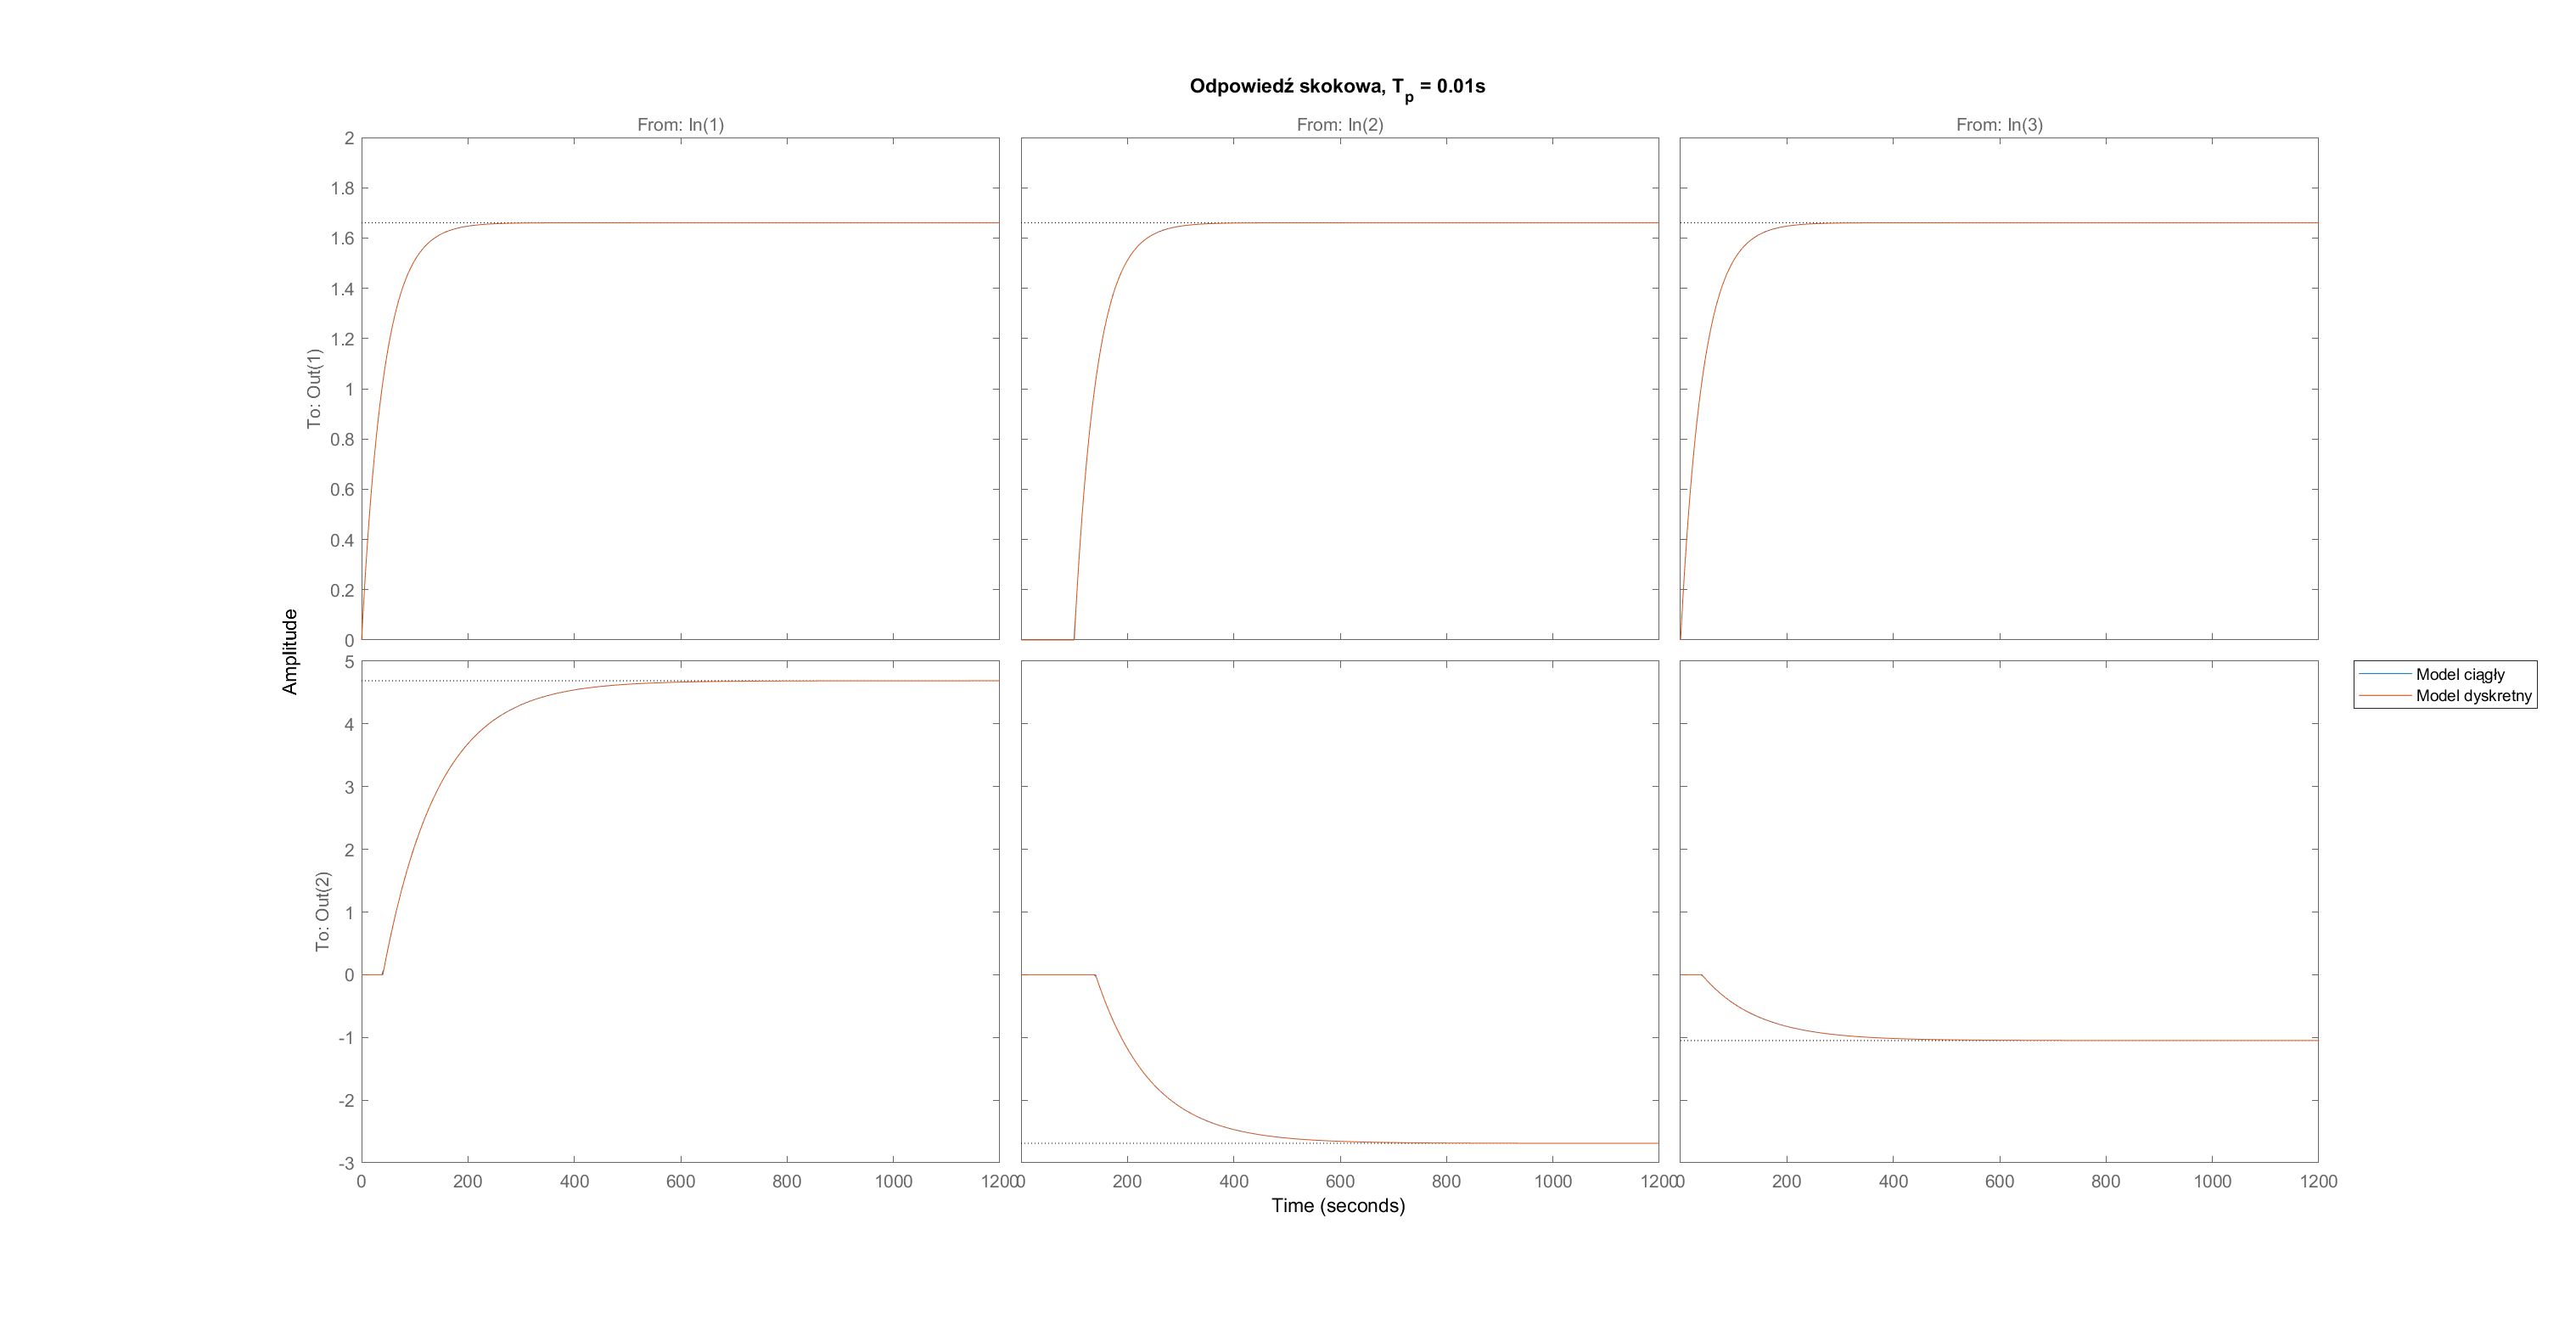
\includegraphics[scale=0.35]{images/stepdt0_01.eps}
    \caption{Odpowiedzi skokowe modeli}
\end{figure}

Z wykresów wyraźnie wynika, że jest konieczny odpowiedni mały krok dyskretyzacji ze względu na szybkie tempo zmian w procesie, stąd też zdecydowano się na krok dyskretyzacji $T_p = 0.1s$.





\end{document}
